%\documentclass{tufte-book}
\documentclass[nofonts,justified,nobib,openany,oneside]{tufte-book}% good in Ubuntu
%                                      'openany' removes blank pages between two chapters, https://stackoverflow.com/a/492148/1173350
%\documentclass[nofonts,justified, nobib]{tufte-book}
%                                 tufte-book modifies the \cite-command heavily, you can turn this behavior off, using the nobib-option:  

\usepackage{cmap} % comment out in Ubuntu


% https://tex.stackexchange.com/a/45949/99685 switch from natbib to biblatex 
\usepackage{hyphenat}

\usepackage[
% citestyle=gost-footnote-min, % wo URL in autocite
  citestyle=gost-footnote, % wo URL in autocite
  bibstyle=gost-footnote,
  citeurl=true,% footnotes and sidenotes with URL
%
%  style=verbose, citepages=omit, % too long title at margins
%  style=authoryear, % e.g. Кузьмина 2021 or Магера 2018.
%  
%  style=authortitle, % Кузьмина, “Аниме:..."
%
%% style=authortitle-ibid,
%%  dashed=false, % in Bibliography dash if authors repeated
%%%%  autolang=other,% multilingual bibliography
  autocite=footnote, 
%%  autopunct=false, % see https://ctan.math.illinois.edu/macros/latex/contrib/biblatex/doc/biblatex.pdf
%                  % a trailing punctuation mark will not be moved against footnote mark
  babel=other, % H. Turki [и др.] -> [et al.]
%  movenames=true, % or false, see https://ctan.math.illinois.edu/macros/latex/contrib/biblatex-contrib/biblatex-gost/doc/biblatex-gost.pdf, page 20
%%  maxcitenames=1,
%  maxbibnames=99, % displaying all authors of multi-author works in the bibliography
  otherlangs=true,
  backend=biber
]{biblatex}
\addbibresource{wd_references.bib}
\ExecuteBibliographyOptions{citetracker=true}

\usepackage{xurl} % break long url, see https://tex.stackexchange.com/a/407368/99685

\usepackage[unicode]{hyperref}

% + shorttitle if twice of more references to the same biblio reference
% https://tex.stackexchange.com/a/26084/99685
\renewbibmacro*{cite:short}{% based on cite:short from verbose.cbx
  \printtext[bibhyperlink]{\printnames{labelname}}%
  \iffieldundef{shorttitle}
    {}
    {\setunit*{\nametitledelim}%
     \printfield[citetitle]{labeltitle}}}

\renewbibmacro*{cite:short}{% based on cite:short from verbose.cbx
  \printtext[bibhyperlink]{\printnames{labelname}}%
  \iffieldundef{shorttitle}
    {}
    {\setunit*{\nametitledelim}%
     \printfield[citetitle]{labeltitle}}}



% source tufte-latex
%\usepackage[T1]{fontenc}
%\usepackage[english,russian]{babel}
%\usepackage[utf8]{inputenc}

% new, see https://tex.stackexchange.com/a/333416
\usepackage[utf8]{inputenc}
\usepackage[T1,T2A]{fontenc} % good in Ubuntu
%\usepackage[T2A]{fontenc}
%\usepackage[russian]{babel} % good in Ubuntu
\usepackage[english,russian]{babel}
%\usepackage[scaled=.85]{PTMono}

%\usepackage[babel=true]{microtype} % good in Ubuntu see https://tex.stackexchange.com/a/355726/99685
\usepackage{csquotes}

% Select font you like
%%%\usepackage{paratype} % very good in Ubuntu
%\usepackage{libertine} % not bad
%%%\usepackage{tempora}  % too heavy


%\usepackage{erewhon} % good bold
%\usepackage{XCharter} % 
\usepackage{cochineal} % good narrow bold best
%\usepackage{lato} % 
%\usepackage{cmsrb} % 
%\usepackage{gentium} % 



%\usepackage{iwona} % so-so
%\usepackage{opensans} % so-so
%\usepackage{droid} % not best - failed
%\usepackage{kurier} % not best
%\usepackage{cantarell} % ? 
%\usepackage{lmodern}

\usepackage{indentfirst} % red entries

% see https://lisakov.com/blog/latex-fonts/
% Шрифты в Latex
%\usepackage{libertine}
%\usepackage{paratype}

%\usepackage{setspace} % see https://tex.stackexchange.com/a/77910/99685
%\doublespacing
% \begin{spacing}{2.5} ... \end{spacing}

% Place footnote in footer in Tufte-book class
% https://tex.stackexchange.com/a/417552/99685
\usepackage{tuftefoot}

% русскоязычные источники предшествовали остальным в Литературе 
\usepackage{biblio-gost-ru-before-en}


% %%%%%%%%%%%%%%%%%%
% todonotes block

\usepackage{xargs} % \newcommandx - see below - Use more than one optional parameter in a new commands

\newcounter{todocounter} 

%see https://tex.stackexchange.com/a/178806/99685
\usepackage[colorinlistoftodos,prependcaption,textsize=large]{todonotes}
\setuptodonotes{inline} % only inline todo notes, without remarks and references at margins

\newcommandx{\todoVlad}[2][1=]{\stepcounter{todocounter}\todo[backgroundcolor=Apricot!25,bordercolor=red,#1]{\thetodocounter: #2}}
\newcommandx{\todoVladWithoutCounter}[2][1=]{\todo[backgroundcolor=Apricot!25,bordercolor=red,#1]{#2}}

\newcommandx{\answerVlad}[2][1=]{\todo[backgroundcolor=Green!25,bordercolor=violet,#1]{#2}}

% eo todonotes block
% %%%%%%%%%%%%%%%%%%


\usepackage{bookmark}% http://ctan.org/pkg/bookmark


% do not add this package, it changes everything drastically
%\usepackage{floatrow}   % Two figures side by side in Tufte-Latex, https://tex.stackexchange.com/a/392927/99685

% How to remove the whitespace BEFORE itemize/enumerate?
\usepackage[shortlabels]{enumitem}% https://tex.stackexchange.com/a/86055/99685

\newenvironment{compactitemize}{%
    \begin{itemize}[noitemsep,topsep=0pt,parsep=0pt,partopsep=0pt]}{\end{itemize}}
%\begin{compactitemize} 

% see https://mydebianblog.blogspot.com/2014/06/latex.html
\usepackage{epigraph} %%% to make inspirational quotes.


% https://tex.stackexchange.com/a/224875/99685
%\usepackage{natbib}           % call natbib
%\setcitestyle{authoryear}     % set citation style to authoryear
%\bibliographystyle{plainnat}  % use the plainnat instead of plain




% documentation: https://mirror.truenetwork.ru/CTAN/macros/latex/contrib/ccaption/ccaption.pdf
%\newcommand{\captiondelim}[1]{\def\@contdelim{#1}}
%\captiondelim{--- }

% source: https://gist.github.com/vsimko/fcc84e1e4f8e750746caa34b802db5a7
\definecolor{LightGray}{rgb}{0.97,0.97,0.97}
\usepackage{soul,listings} % syntax highlighting
\usepackage{xparse} % insert code keywords inline, see https://tex.stackexchange.com/a/286097/99685


% Listing N: Title -> Query N. Title
% before \usepackage{listings}
\renewcommand{\lstlistingname}{Запрос}  % Листинг -> Запрос
%\renewcommand{\lstlistingname}{Листинг} % Запрос -> Листинг

\makeatletter
\long\def\@makecaption#1#2{%
%    \renewcommand{\lstlistingname{\protect\text{Query}}}{}
    \renewcommand{\lstlistingname}{Запрос}
\centering%
#1. #2\par%
%XX1#1.XX2 YY1#2YY2\par%
\vspace{\belowcaptionskip}% too large vertical gap
\vspace{5pt}% vertical distance from Request title the source code
}%
\makeatother

% Listing -> Query
%\renewcommand\lstlistingname{Запрос}

\lstdefinelanguage{SPARQL}{%
  texcl=true,
  basicstyle=\small\ttfamily,
  backgroundcolor=\color{LightGray},
  columns=fullflexible,
  breaklines=false,
  sensitive=true,
  % --------------------------
  frame=bt, % bottom and top lines
  aboveskip=1em,
  belowskip=1em,
  xleftmargin=.5em,
  xrightmargin=.5em,
  framexleftmargin=.5em,
  framextopmargin=.5em,
  framexbottommargin=.5em,
  framexrightmargin=.5em,
  % --------------------------
  tabsize = 2,
  showstringspaces=false,
  morecomment=[l][\color{gray}]{\#},       % comments
  morecomment=[n][\color{blue}]{<http}{>}, % uris
  morestring=[b][\color{OliveGreen}]{\"},  % strings
  % -------------------------- variables
  keywordsprefix=?,
  classoffset=0,
  keywordstyle=\color{Sepia},
  morekeywords={},
  % -------------------------- prefixes
  classoffset=1,
  keywordstyle=\color{Purple},
  morekeywords={rdf,rdfs,owl,xsd,purl},
  % -------------------------- keywords
  classoffset=2,
  keywordstyle=\color{MidnightBlue},
  morekeywords={
    SELECT,CONSTRUCT,DESCRIBE,ASK,WHERE,FROM,NAMED,PREFIX,BASE,OPTIONAL,
    FILTER,GRAPH,LIMIT,OFFSET,SERVICE,UNION,EXISTS,NOT,BINDINGS,MINUS,a
  },
  %\lst@ifdisplaystyle\scriptsize\fi
}
%\lstset{language=SPARQL,frame=lines}

\lstloadlanguages{Python}
\input{listings-python.prf}
\lstset{%
   language=Python,
   texcl=true,
   extendedchars=\true,
   keepspaces=true,
   frame=bt,
   basicstyle=\small\ttfamily,
   backgroundcolor=\color{LightGray},
   showstringspaces=false,
   showspaces=false,
   numbers=none,
   tabsize=2,
   breaklines=true,
   keywordstyle=\color{Sepia},
   stringstyle=\color{OliveGreen}
%   captionpos=b
}
% see https://alexanius-blog.blogspot.com/2012/09/lstlistings.html
% extendedchars=\true,


% color row in table via \rowcolor{LightCyan}
% https://texblog.org/2011/04/19/highlight-table-rowscolumns-with-color/
\definecolor{LightCyan}{rgb}{0.88,1,1}
\usepackage{colortbl}

% see https://tex.stackexchange.com/a/79985/99685
\usepackage{siunitx}[=v2] % \num{12345,67890}


% links to Russian Wikipedia articles \ruwiki{short w.wiki link}{Москва}
% for example \ruwiki{vDw}{МиГ} = \href{https://w.wiki/vDw}{МиГ}
% see https://tex.stackexchange.com/a/86368/99685
\usepackage{texlinks} 
%\newcommand*{\ruwiki}{\wikilangref{ru}} - failed cyrillic in URL
% \href{https://w.wiki/vDw}{МиГ} -> \ruwiki{vDw}{МиГ}
\newcommand{\ruwiki}[2]{\href{https://w.wiki/#1}{#2}}

% full link to short URL created by URL Shortener, 
% e.g. \wwiki{XYZ} = \href{https://w.wiki/XYZ}{https://w.wiki/XYZ}
\newcommand{\wwiki}[1]{\href{https://w.wiki/#1}{https://w.wiki/#1}}

% two parameters in case of special symbols in URL, e.g. $ = %24
% e.g. \wwiki{X\%24Z}{X$Y} = \href{https://w.wiki/X\%24Z}{https://w.wiki/X$Z}
% \newcommand{\wwiki}[1]{\href{https://w.wiki/#1}{https://w.wiki/#1}} or better is the explicit command?


% Wikidata object hyperlink in the form: QID, e.g. Q312154
\newcommand{\wdq}[1]{\href{https://www.wikidata.org/wiki/Q#1}{Q#1}}
% Wikidata object hyperlink in the form: Name (QID), e.g. Drosophila (Q312154)
\newcommand{\wdqName}[2]{\href{https://www.wikidata.org/wiki/Q#2}{#1~(Q#2)}}

% Wikidata object property name and hyperlink
% \wdproperty{ID}{Name} = \href{https://www.wikidata.org/wiki/Property:PID}{Name (PID)}
\newcommand{\wdProperty}[2]{\href{https://www.wikidata.org/wiki/Property:P#1}{#2 (P#1)}}

% How to add a forced line break inside a table cell
% https://tex.stackexchange.com/a/19678
\newcommand{\specialcell}[2][c]{%
  \begin{tabular}[#1]{@{}c@{}}#2\end{tabular}}


% comment all in Ubuntu
%\renewcommand{\rmdefault}{cmr} % CM roman
%\renewcommand{\sfdefault}{cmss} % CM sans serif 
%\renewcommand{\ttdefault}{cmtt} % CM monospaced 

%\renewcommand{\rmdefault}{ptm} % Times 
%\renewcommand{\sfdefault}{phv}
%\renewcommand{\ttdefault}{pcr}




%%% Draft (debug) or release version of the book
\makeatletter
\@ifundefined{c@draft}{
  \newcounter{draft}
  \setcounter{draft}{1} % 0 --- clean release version, without any comments, 
}{}                     %       with only finished chapters.
\makeatother            % 1 --- draft version, unfinished chapters included, 
                        %       with questions and comments
%%% eo Draft or release




% Remove prefix from figure caption in tufte-book, see https://tex.stackexchange.com/a/106422/99685
%\makeatletter
%\newenvironment{nocapfigure}
%  {\let\H@refstepcounter\@gobble%
%   \long\def\@caption##1[##2]##3{%
%   \par%
   %\addcontentsline{\csname ext@##1\endcsname}{##1}%
   %  {\protect\numberline{\csname the##1\endcsname}{\ignorespaces ##2}}%
%   \begingroup%
%     \@parboxrestore%
%     \if@minipage%
%       \@setminipage%
%     \fi%
%     \@tufte@caption@font\@tufte@caption@justification%
%     \noindent\ignorespaces##3\par%\noindent\csname fnum@#1\endcsname: \ignorespaces#3\par%
     %\@makecaption{\csname fnum@#1\endcsname}{\ignorespaces #3}\par
%   \endgroup}\figure
%    }{\endfigure}
%\makeatother



% -> "Рис. 8.4. Карта соседних стран..."
%\makeatletter
%\long\def\@caption#1[#2]#3{%
%  \par
%  \addcontentsline{\csname ext@#1\endcsname}{#1}%
%    {\protect\numberline{\csname the#1\endcsname}{\ignorespaces #2}}%
%  \begingroup
%    \@parboxrestore
%    \if@minipage
%      \@setminipage
%    \fi
%    \@tufte@caption@font\@tufte@caption@justification
%    \noindent\csname fnum@#1\endcsname. \ignorespaces#3\par% changed : to .
%%    \noindent ss \csname fnum@#1\endcsname. ll \ignorespaces#3 ii\par% changed : to .
%  \endgroup}
%\makeatother




% If too much notes: see https://tex.stackexchange.com/a/175796/99685
%\usepackage{marginfix}

% how to use `\marginnote` in `mdframed` environment?, see https://tex.stackexchange.com/a/412839/99685
\usepackage[framemethod=TikZ]{mdframed}
\usepackage{twemojis}% used in items in Chapter. Advanced. Защита страниц
%%% $\twemoji[width=24pt]{computer}$\,\, 

%\let\marginnote\someundefinedcommand
%\usepackage{marginnote}

%\newmdenv[skipabove=6mm]{mdfstyle}

\hypersetup{colorlinks}% uncomment this line if you prefer colored hyperlinks (e.g., for onscreen viewing)
%\usepackage{breakurl}% see https://tex.stackexchange.com/a/21266/99685

\setcounter{secnumdepth}{0} % turn on numbering for parts and chapters 

\usepackage{amsthm, amsmath, amssymb}
%\usepackage{setspace, enumerate}

\usepackage[linesnumbered,boxed]{algorithm2e}
\newcommand{\var}{\texttt} % for names of variables in plain text https://tex.stackexchange.com/a/381105/99685

\newtheoremstyle{definition}%
{}
{}
{}%{\itshape}%bodyfont
{}%indent
{}%{\bfseries}%headfont
{}%head punctuation
{ }% space after head - e.g. \parindent paragraph indent before Answer.
{}

\theoremstyle{definition}
\newtheorem*{task}{} % numbering of tasks in the section: Answers

%%
% Book metadata
\title{Программирование \\Викиданных}% \\для школьников \\и студентов}
\author[Крижановский и др.]{Крижановский Андрей, Балакирева Мария, Меньшикова Екатерина, \mbox{Паренченков Евгений}, Потес Артём, Трубина Елизавета, \mbox{Обрегон Анхель}}
%\author[Крижановский А. А., Балакирева М. С., Меньшикова Е. А., Паренченков Е. О., Потес А. С., Трубина Е. Д.]{Крижановский Андрей, Балакирева Мария, Меньшикова Екатерина, Паренченков Евгений, Потес Артём, Трубина Елизавета}
%\author[Крижановский Андрей, Иванов Иван]{Крижановский Андрей,\ Иванов Иван,\ добавьте свою фамилию и имя ...}
\publisher{Петрозаводский государственный университет,\\Карельский научный центр РАН}

%%
% If they're installed, use Bergamo and Chantilly from www.fontsite.com.
% They're clones of Bembo and Gill Sans, respectively.
%\IfFileExists{bergamo.sty}{\usepackage[osf]{bergamo}}{}% Bembo
%\IfFileExists{chantill.sty}{\usepackage{chantill}}{}% Gill Sans

%\usepackage{microtype}

%%
% Just some sample text
%\usepackage{lipsum}


% table of contents: tocloft
\usepackage{tocloft}
\renewcommand{\cfttoctitlefont}{\huge} % The header "Contents"/"Оглавление" font size (not so huge as default)
\renewcommand\cftchapaftersnum{.}% adds dot after chapter title in ToC
\renewcommand\cftchapdotsep{\cftdotsep}% adds leader dots from chapter titles to page numbers
%\makeatletter \renewcommand{\@dotsep}{4.5} \makeatother % + dots in Table of contents

% "Часть" + \part{} + "."
\dottedcontents{part}[0em]{\sffamily\bfseries\large\protect\addvspace{15pt}Часть}{-5pt}{1pc}
\renewcommand{\thepart}{\Roman{part}.}  % adds dot after part title in ToC

% separate page with "Part II \newline ornament \newline The part title
\usepackage{pgfornament}
\newcommand{\formatpart}[1]{%
    \begin{fullwidth}
    \centering
%    \partname~\thepart%
    \partname~\Roman{part}% without dot at the end: "Part I", not "Part I."

    \vspace*{0.2\baselineskip}
    \pgfornament[width=4cm, color=Sepia]{69}%
    \vspace*{0.5\baselineskip}

    #1%
    \end{fullwidth}%
%    \centering\includegraphics[width=38pt]{./Big-bot-icon.png}
}



\titleformat% Formatting the part header 
  {\part} % command
  [block] % shape
  {\bfseries\sc\Huge} % format todo
  {} % label
  {0pt} % sep - moving "Chapter" to right (to center)
  {\formatpart}

\usepackage{figchild}
\newcommand{\MarginQuestion}{% Lamp image from the package figchild, in the beginning of the questions on margins
\noindent\reflectbox{{% Mirroring the lamp to right (to a question text)
\fcTableLight{0.1}{black}{1}%
}}%
}
\newcommand{\MarginInternalLink}{% Pencil image, reference to other sections
\noindent\reflectbox{{% Mirroring the lamp to right (to a question text)
\fcPencilA{0.06}{black}{1}%
}}\,\,\,% % some space \,%
}

\newcommand{\MarginNB}{% rocket image, Attention, NotaBene
\noindent\fcRocketA{0.1}{black}{1}%
\,\,\,% % some space \,%
}



%\fcBinoculars{0.1}{black}{1}
%\fcFlyingSaucer{0.6}{black}{1}
%\fcPuppy{0.1}{black}{1}
%\fcSeahorse{0.1}{black}{1}

%%
% For nicely typeset tabular material
\usepackage{booktabs}

%%
% For graphics / images
\usepackage{graphicx}
\setkeys{Gin}{width=\linewidth,totalheight=\textheight,keepaspectratio}
\graphicspath{{graphics/}}


% The fancyvrb package lets us customize the formatting of verbatim
% environments.  We use a slightly smaller font.
% \usepackage{fancyvrb}
% \fvset{fontsize=\normalsize}

%%
% Prints argument within hanging parentheses (i.e., parentheses that take
% up no horizontal space).  Useful in tabular environments.
\newcommand{\hangp}[1]{\makebox[0pt][r]{(}#1\makebox[0pt][l]{)}}

%%
% Prints an asterisk that takes up no horizontal space.
% Useful in tabular environments.
\newcommand{\hangstar}{\makebox[0pt][l]{*}}

%%
% Prints a trailing space in a smart way.
\usepackage{xspace}

% $\blackinwhitediamond$ in Answers
\usepackage[notextcomp]{stix} % notexcomp since textcomp is loaded in tufte-common.def
\newcommand{\AnswerBackref}{% 
$\blackinwhitediamond$ %
}



%%
% Some shortcuts for Tufte's book titles.  The lowercase commands will
% produce the initials of the book title in italics.  The all-caps commands
% will print out the full title of the book in italics.
\newcommand{\vdqi}{\textit{VDQI}\xspace}
\newcommand{\ei}{\textit{EI}\xspace}
\newcommand{\ve}{\textit{VE}\xspace}
\newcommand{\be}{\textit{BE}\xspace}
\newcommand{\VDQI}{\textit{The Visual Display of Quantitative Information}\xspace}
\newcommand{\EI}{\textit{Envisioning Information}\xspace}
\newcommand{\VE}{\textit{Visual Explanations}\xspace}
\newcommand{\BE}{\textit{Beautiful Evidence}\xspace}

\newcommand{\TL}{Tufte-\LaTeX\xspace}

% Prints the month name (e.g., January) and the year (e.g., 2008)
\newcommand{\monthyear}{%
  \ifcase\month\or January\or February\or March\or April\or May\or June\or
  July\or August\or September\or October\or November\or
  December\fi\space\number\year
}



% Inserts a blank page
\newcommand{\blankpage}{\newpage\hbox{}\thispagestyle{empty}\newpage}

\usepackage{units}

% Typesets the font size, leading, and measure in the form of 10/12x26 pc.
\newcommand{\measure}[3]{#1/#2$\times$\unit[#3]{pc}}

% Macros for typesetting the documentation
\newcommand{\hlred}[1]{\textcolor{Maroon}{#1}}% prints in red
\newcommand{\hangleft}[1]{\makebox[0pt][r]{#1}}
\newcommand{\hairsp}{\hspace{1pt}}% hair space
\newcommand{\hquad}{\hskip0.5em\relax}% half quad space
\newcommand{\TODO}{\textcolor{red}{\bf TODO!}\xspace}
\newcommand{\na}{\quad--}% used in tables for N/A cells
\providecommand{\XeLaTeX}{X\lower.5ex\hbox{\kern-0.15em\reflectbox{E}}\kern-0.1em\LaTeX}
\newcommand{\tXeLaTeX}{\XeLaTeX\index{XeLaTeX@\protect\XeLaTeX}}
% \index{\texttt{\textbackslash xyz}@\hangleft{\texttt{\textbackslash}}\texttt{xyz}}
\newcommand{\tuftebs}{\symbol{'134}}% a backslash in tt type in OT1/T1
\newcommand{\doccmdnoindex}[2][]{\texttt{\tuftebs#2}}% command name -- adds backslash automatically (and doesn't add cmd to the index)
\newcommand{\doccmddef}[2][]{%
  \hlred{\texttt{\tuftebs#2}}\label{cmd:#2}%
  \ifthenelse{\isempty{#1}}%
    {% add the command to the index
      \index{#2 command@\protect\hangleft{\texttt{\tuftebs}}\texttt{#2}}% command name
    }%
    {% add the command and package to the index
      \index{#2 command@\protect\hangleft{\texttt{\tuftebs}}\texttt{#2} (\texttt{#1} package)}% command name
      \index{#1 package@\texttt{#1} package}\index{packages!#1@\texttt{#1}}% package name
    }%
}% command name -- adds backslash automatically
\newcommand{\doccmd}[2][]{%
  \texttt{\tuftebs#2}%
  \ifthenelse{\isempty{#1}}%
    {% add the command to the index
      \index{#2 command@\protect\hangleft{\texttt{\tuftebs}}\texttt{#2}}% command name
    }%
    {% add the command and package to the index
      \index{#2 command@\protect\hangleft{\texttt{\tuftebs}}\texttt{#2} (\texttt{#1} package)}% command name
      \index{#1 package@\texttt{#1} package}\index{packages!#1@\texttt{#1}}% package name
    }%
}% command name -- adds backslash automatically
\newcommand{\docopt}[1]{\ensuremath{\langle}\textrm{\textit{#1}}\ensuremath{\rangle}}% optional command argument
\newcommand{\docarg}[1]{\textrm{\textit{#1}}}% (required) command argument
\newenvironment{docspec}{\begin{quotation}\ttfamily\parskip0pt\parindent0pt\ignorespaces}{\end{quotation}}% command specification environment
\newcommand{\docenv}[1]{\texttt{#1}\index{#1 environment@\texttt{#1} environment}\index{environments!#1@\texttt{#1}}}% environment name
\newcommand{\docenvdef}[1]{\hlred{\texttt{#1}}\label{env:#1}\index{#1 environment@\texttt{#1} environment}\index{environments!#1@\texttt{#1}}}% environment name
\newcommand{\docpkg}[1]{\texttt{#1}\index{#1 package@\texttt{#1} package}\index{packages!#1@\texttt{#1}}}% package name
\newcommand{\doccls}[1]{\texttt{#1}}% document class name
\newcommand{\docclsopt}[1]{\texttt{#1}\index{#1 class option@\texttt{#1} class option}\index{class options!#1@\texttt{#1}}}% document class option name
\newcommand{\docclsoptdef}[1]{\hlred{\texttt{#1}}\label{clsopt:#1}\index{#1 class option@\texttt{#1} class option}\index{class options!#1@\texttt{#1}}}% document class option name defined
\newcommand{\docmsg}[2]{\bigskip\begin{fullwidth}\noindent\ttfamily#1\end{fullwidth}\medskip\par\noindent#2}
\newcommand{\docfilehook}[2]{\texttt{#1}\index{file hooks!#2}\index{#1@\texttt{#1}}}
\newcommand{\doccounter}[1]{\texttt{#1}\index{#1 counter@\texttt{#1} counter}}


% Tufte book in landscape
% https://tex.stackexchange.com/a/413441/99685
% text the same width, margin width ++
%\geometry{a4paper,landscape,left=24.8mm,top=27.4mm,headsep=2\baselineskip,textwidth=107mm,marginparsep=8.2mm,marginparwidth=136.4mm,textheight=34\baselineskip,headheight=\baselineskip}
% text = 107 mm (old) + 40 mm = 147, margin = 49.4 mm (old) + 47 = 96.4 mm
\geometry{a4paper,landscape,left=24.8mm,top=27.4mm,headsep=2\baselineskip,textwidth=147mm,marginparsep=8.2mm,marginparwidth=96.4mm,textheight=34\baselineskip,headheight=\baselineskip}


% Absolutely, definitely, preventing page break, https://tex.stackexchange.com/a/94702/99685
%\newenvironment{absolutelynopagebreak}
%  {\par\nobreak\vfil\penalty0\vfilneg
%   \vtop\bgroup}
%  {\par\xdef\tpd{\the\prevdepth}\egroup
%   \prevdepth=\tpd}


% Generates the index
\usepackage{makeidx}
\makeindex

\begin{document}
\sisetup{mode=text} % Trying to get the same font when using SI units in text and math mode 

% Front matter
%\frontmatter

% r.1 blank page
%\blankpage

% r.3 full title page
\maketitle


%%%%%%%%%%%%%%%%%%%%%%%%%%%%%%%%%%%
% Let's comment out this page 
%\iffalse

% v.4 copyright page
\newpage
\begin{fullwidth}
УДК 004 \\
ББК 32.973 \\
\hphantom{ББК} П784
~\vfill
\thispagestyle{empty}
\setlength{\parindent}{0pt}
\setlength{\parskip}{\baselineskip}

Это учебник по Викиданным и языку SPARQL. 
Викиданные~--- это огромная база данных, лежащая в основе Википедии и связывающая вики-проекты воедино.
Прочитав книгу, вы сможете извлекать из Викиданных информацию с~помощью SPARQL-скриптов, 
затем обрабатывать её и строить по ней таблицы, графики и карты. \\ 
Учебник предназначен для студентов, %Института математики и информационных технологий ПетрГУ, 
изучающих информатику, 
для тех, кто хочет развить свои аналитические навыки, 
    научиться программировать 
    и глубже разбираться в принципах работы самого компьютерного вики-проекта. \\
%Книга писалась одновременно с созданием учебного курса <<Программирование Викиданных>> в Викиверситете. 
    Дополнительные материалы доступны онлайн 
    (\href{https://w.wiki/62E}{https://ru.wikiversity.org/wiki/Программирование\_Викиданных}) 
    в одноимённом курсе Викиверситета.
Учебник распространяется на правах свободной лицензии 
    \href{https://creativecommons.org/licenses/by-sa/4.0/deed.ru}{Creative Commons Attribution-ShareAlike}.

Copyleft \textcopyleft\ \the\year\ \thanklessauthor

%\par\smallcaps{Published by \thanklesspublisher}
%\par\smallcaps{\thanklesspublisher}
\par{\thanklesspublisher}

%\par\textit{First printing, \monthyear}


\end{fullwidth}
\newpage
%\fi 
\begin{fullwidth}
% eo of commented out page
%%%%%%%%%%%%%%%%%%%%%%%%%%



% r.5 contents
\tableofcontents

\end{fullwidth}


% r.7 dedication
\clearpage
\vfill
\begin{fullwidth}

% a small hack to fix the hsize, to align epigraph block right
% https://stackoverflow.com/a/31522918/1173350
\makeatletter\setlength\hsize{\@tufte@fullwidth}\makeatother

\renewcommand{\epigraphsize}{\Large}
\renewcommand{\epigraphflush}{flushright}
\setlength{\epigraphwidth}{.7\linewidth}

\epigraph{Что может быть проще примитивного нуль-передатчика? Только примитивный нуль-аккумулятор.}%
{\fontfamily{iwona}\selectfont%
\textit{Обитаемый остров\\Аркадий и Борис Стругацкие}%
}%eo fontfamily

\vspace{36px}

\epigraph{%
Эта машина, подпиравшая стены железными боками, была огромна. Электроник, поглощая цифры, скоро пришёл к выводу, что ему нужно сидеть здесь несколько суток\dots\\
---~Я всего этого не запомню,~--- скрипуче сказал Электроник. ---~Миллионы цифр! Слишком большое количество информации\dots\\
Профессор положил руку на его плечо.\\
---~Отключись,~--- посоветовал он. ---~Привыкать надо постепенно.}%
{\fontfamily{iwona}\selectfont%
\textit{Рэсси~--- неуловимый друг\\Евгений Велтистов}%
}%eo fontfamily

    
\vspace{56px}


\setlength{\epigraphrule}{0pt} % rm the rule (line)
\epigraph{%
{\fontfamily{iwona}\selectfont%
\textit{\textbf{Издание посвящается изобретателям SPARQL-скриптов~--- программистам будущего, 
а~также OSINT-разведчикам, для которых Викиданные будут школьным полигоном}}%
}%eo fontfamily
}{}
\end{fullwidth}


% r.9 introduction
%\cleardoublepage

\chapter*{Введение}
\label{ch:intro}

\newthought{Эта книга} предназначена для школьников и студентов. 
Вы познакомитесь с работой базы Викиданных и языком запросов SPARQL, 
с помощью которого можно работать с этой базой. 
Прочитав книгу, вы сможете извлекать из Викиданных информацию с~помощью SPARQL-скриптов, 
затем обрабатывать её и строить по ней таблицы, графики и карты.

\newthought{Цель} этой книги быть учебником по Викиданным и языку SPARQL.

\vspace{4mm}

Викиданные~--- это искусно сделанная база данных, которая как огромный кит лежит в основе громадной планеты Википедии\marginnote{%
%
Подробнее о Викиданных читайте главу <<\nameref{ch:ReviewAboutWD}>> на с.~\pageref{ch:ReviewAboutWD}
%
}. 
Впечатляет скорость роста этого кита, во многих главах мы будем обращать на это внимание.
Если изначально Викиданные создавались для обслуживания нужд Википедии, 
то сейчас Викиданные используются крайне широко и в самых разных целях.

\vspace{4mm}
Опишем структуру книги. 

\newthought{В первой части книги}\marginnote{%
%
Часть <<\nameref{part:foundation}>> на с.~\pageref{part:foundation}
%
} описано, 
что такое листинги программ, как ими пользоваться, даны базовые понятия об объектах Викиданных. 
Кратко рассказано о сервисе балансировки ProWD. 
Большая глава <<Обзор Викиданных>> включает историческую справку, 
вопрос качества данных и связи с Википедией. 
Описан сервис WDQS, к которому мы будем обращаться на каждой странице. 
Также включён небольшой обзор научных исследований, связанных с Викиданными. 
Глава <<Корзины и мячи>> с помощью образов и аналогий позволяет подступиться к Викиданным тем, 
кто хочет научиться программировать. 

%включает в себя 10 уроков, описывающих язык программирования и протокол SPARQL.
%\newthought{Вторая часть} содержит рецепты решения самых разных практических задач, 
%возникающих при работе с объектами Викиданных.

\newthought{Во второй и основной части}\marginnote{%
%
Часть <<\nameref{part:research}>> на с.~\pageref{part:research}
%
} 
каждая глава~--- это небольшое приключение, 
где один из объектов Викиданных является главным героем. 
С помощью SPARQL-запросов мы пытаемся расспросить Викиданные об этом герое, 
с помощью графиков, таблиц, диаграмм проанализировать и нарисовать себе его образ. 

\newthought{В третьей части}\marginnote{%
%
Часть <<\nameref{part:advanced}>> на с.~\pageref{part:advanced}
%
} % 
 рассмотрен вопрос защиты страниц в вики-проектах и то, как последовательно от SPARQL-запросов 
к языку Python можно двигаться при создании компьютерных программ (ботов), редактирующих Викиданные. 

\newthought{Заключительный раздел}\marginnote{%
%
Часть <<\nameref{part:conclusion}>> на с.~\pageref{part:conclusion}
%
} % 
собрал ответы на вопросы, рассеянные по всей книге, список литературы 
и индекс ключевых слов для удобного постраничного поиска.

\newthought{В исследованиях} объектов Викиданных приняли участие студенты ПетрГУ в рамках курса <<Программирование Викиданных>>, 
представленного на сайте Викиверситет\marginnote{%
todo add link
}. 
Этот курс растёт и пишется вместе с этой книгой. 

Потребовалось несколько лет работы со студентами в Википедии, прежде чем мы пришли с ними к таким проектам, 
как Викиверситет и Викиданные. 
Результатом предыдущей работы в Википедии стало учебное пособие для тех, 
кто хочет научиться редактировать мировую энциклопедию\autocite{Krizhanovsky2015}.

% \newthought{Книга научит} вас делать ... todo
%\vspace{5mm}

\newthought{Почему мы занялись и увлеклись Викиданными?}

Потому что это самая большая, сложная 
и быстрорастушая база данных на Земле. 
Потому что эта база лежит в основе Википедии, которую может редактировать каждый.
И Викиданные тоже может редактировать каждый. 

Работу серверов Википедии и Викиданных обеспечивают сотрудники организации Викимедиа. 
Не всё у разработчиков программ и сотрудников Фонда Викимедиа получается хорошо\marginnote{%
%
Сергей Рублёв: 
    <<Удивительно как что-то там работает вообще. На святом духе, как говорят русские.
    Когда Красоткин своих ботов разогнал, обнаружилось, как сказал Неолекс, что: 
    движок всей Викимедии это на сейчас $=\sim$ детский трёхколёсный велосипед с крыльями и реактивным двигателем. 
    На котором мы все (Википедию включая) отважно летим к звёздам. 
    В таком путешествии главное~--- ``не раскачивать лодку''.>> 
    \it{Сергей Рублёв, Александр Красоткин и Neolexx~--- 
    это вики-интеллегенция, то есть редакторы вики-проектов. 
    О ботах Викиновостей см. заметку} <<Фонд Викимедиа сломал Русские Викиновости>>, URL: \href{https://w.wiki/33d8}{w.wiki/33d8}.%
}, 
но другой Википедии у нас нет.

\newthought{Будет ли в этой книге рассказано}, 
как редактировать и пополнять Викиданные новой информацией? 

Нет, хотя это не сложнее, чем писать текст в SMS 
или статью в Википедии. В этом учебнике мы покажем вам, 
как задавать вопросы на языке этой базы, 
чтобы вы ориентировались в ней лучше, чем у себя дома. 

\newthought{Почему школьники?} 

Потому что вообще программирование и программирование Викиданных в частности~--- это 
увлекательная и, если увлечься, простая вещь. 
Если с помощью учителя или самостоятельно школьник увлечётся, 
то сможет программировать Викиданные, писать статьи Википедии. 
Есть десятки школьников, плодотворно работающих в Википедии. 
Надеемся, что благодаря этой книги одним из первых языков, 
изучаемых по информатике в~школе, станет язык Викиданных.

Покажем прямо сейчас, что Викиданные находятся от нас на расстоянии одного клика.
Откройте на компьютере или на телефоне такую ссылку: 
\url{https://w.wiki/4cXU}. 
Вы увидите главное окно, в котором мы с вами будем писать наши небольшие програмы. 
Если вы нажмёте большую синюю кнопку с белым треугольником, 
    \marginnote[0cm]{
    TODO Добавить картинку с кнопкой на поля
    }
то запустите 
эту программу из семи строк. Программа обратится к базе данных 
и спросит, какие столицы есть в Викиданных?
Результатом будет список столиц.\marginnote{%
%
Подробный рассказ о том, что можно узнать и подсчитать о городах в Викиданных,  
читайте в главе <<\nameref{ch:city}>> на с.~\pageref{ch:city}. 
} % 
Вот так просто можно запускать программы в этой книге: достаточно браузера, 
Интернета и гиперссылки с запросом к Викиданным.


%%
% Start the main matter (normal chapters)
\mainmatter






\part{Основы Викиданных}%
\label{part:foundation}%


\iffalse

\section{About listings}
\labsec{section:listing-about}

This book contains listings in SPARQL scripts.
These scripts extract and process data from Wikidata.%\todo{To add screenshot to this (?) sidenote.}

An example SPARQL script is shown in (Listing~\ref{lst:cities}). 
This script gets a list of cities from Wikidata, 
namely: instances of object \wdqName{city}{515}.
The colored text in the listing title (\href{https://w.wiki/ktn}{List of cities}) 
is the link to the corresponding SPARQL script online, 
which is available online: 
% todo \href{https://w.wiki/ktn}{w.wiki/ktn}\sidenote[?]{How did we get such a short link to the script?}


%точнее экземляров объекта\footnote{\label{question:instance-in-OOP-vs-Wikidata}Что такое экземпляр объекта? 
%    Какая разница между экземпляром объекта 
%    в объектно-ориентированном программировании и в Викиданных?
%    См. ответ~\ref{answer:instance-in-OOP-vs-Wikidata} на с.~\pageref{answer:instance-in-OOP-vs-Wikidata}.
%    }

\begin{lstlisting}[ language=SPARQL, 
                    caption={\href{https://w.wiki/ktn}{List of cities}\\\hspace{\textwidth}
                        The result contains \num{20 800} cities in 2017, 
                        \num{9 260} cities in 2020.},
                    label=lst:cities,
                    texcl 
                    ]
SELECT ?city ?cityLabel WHERE { 
  ?city wdt:P31 wd:Q515.       # instance of city 
  SERVICE wikibase:label { bd:serviceParam wikibase:language "en" }
}
\end{lstlisting}%
%\footnotetext{The result contains \num{20 800} cities in 2017 year, 
%    \num{9 260} cities in 2020.}




\chapter{Обзор Викиданных}
\label{ch:ReviewAboutWD}

\section{Викиданные}

Викиданные~--- это структурированная и совместно редактируемая база данных\footnote[][-15pt]{Викиданные (Wikidata)~--- это свободная, совместно наполняемая, многоязычная, вторичная база данных, в которой собрана структурированная информация для поддержки работы Википедии, Викисклада и других проектов Викимедиа.}. Проект был официально запущен 30 октября 2012 года, его разработка ведётся под руководством Wikimedia Deutschland\footnote[][5pt]{Немецкое отделение Фонда Викимедиа.}. Проект создавался за счёт пожертвований Allen Institute for Artificial Intelligence, Gordon and Betty Moore Foundation и Google. Викиданные~--- это бесплатная и свободная база знаний, которая может использоваться и редактироваться людьми и компьютерными программами\autocite{Vrandecic}.\begin{marginfigure}[0.0cm]
{
	\setlength{\fboxsep}{0pt}%
	\setlength{\fboxrule}{1pt}%
	\fcolorbox{gray}{white}{\includegraphics[width=0.41\linewidth]{./review/Wikidata-logo-en.png}}
}
\caption[Логотип Викиданных]{Логотип Викиданных. 
Wikimedia Commons / \href{https://commons.wikimedia.org/wiki/File:Wikidata-logo-en.svg}{Planemad} 
}
\label{fig:seyu}
\end{marginfigure}

Содержимое Викиданных распространяется по лицензии Creative Commons CC0, которая позволяет повторно использовать информацию самыми разными способами: пользователи могут копировать, изменять, распространять и обрабатывать эти данные в любых целях. Ещё одна особенность Викиданных~--- это многоязычность. Любой человек может редактировать Викиданные более чем на 350 языках.

Викиданные постоянно обновляются, добавляются новые объекты. 
На 2023 год насчитывается более 100 млн страниц и около 2 млрд правок 
(данные взяты с официальной страницы статистики Викиданных: 
\href{https://www.wikidata.org/wiki/Wikidata:Statistics}{https://www.wikidata.org/wiki/Wikidata:Statistics}). 
Уже в 2019 году на сайте Викиданных было совершено более 800 тыс. правок, что превзошло количество правок в Английской Википедии и сделало Викиданные наиболее редактируемым сайтом Викимедиа. %\footnote[][5px]{
Веб-сайт Викиданных, к которому мы будем регулярно обращаться, такой: \href{https://www.wikidata.org}{https://www.wikidata.org}. %}.




\section{Wikidata Query Service}
\label{sect:WDQS}
\index{Wikidata Query Service}

Любой объект Викиданных имеет свой уникальный идентификатор и свойства. 
Эта информация может быть обработана с помощью компьютера, 
и при этом она наглядно представлена и понятна пользователям без специальной предобработки. 
Сайт Викиданных содержит сервис Wikidata Query\footnote{%
%
Полное название инструмента Wikidata Query Service, кратко~--- WDQS. URL: 
\href{https://query.wikidata.org/}{https://query.wikidata.org/}.%
%
}, включающий набор инструментов для построения SPARQL-запросов 
и их визуализации в~виде таблиц, диаграмм, графов или географических карт.
\index{Wikidata Query Service}



\section{Об исследовании Викиданных}

В работе \textit{A large-scale collaborative ontological medical database}\footnote{%
\fullcite{Collaborative_ontological_database}.}\,описываются плюсы использования Викиданных для создания крупномасштабной 
совместно используемой медицинской базы данных. 
Основные требования к создаваемой базе данных таковы: 
это должна быть платформа с~обновлением в~реальном времени, 
с~лицензией, разрешающей дальнейшее использование полученной информации, 
с~возможностью редактирования на~любом языке и с~открытым доступом. 
Именно это и есть основные характеристики Викиданных. 
Во-первых, Викиданные~--- это открытая, редактируемая база знаний. 
Любой пользователь без навыков программирования может вносить изменения 
более чем на 350 языках. 
Во-вторых, информация постоянно обновляется, добавляются новые объекты. 
На~2023 год Викиданные насчитывают около 25~тыс. редакторов\footnote{Для сравнения: 
число активных редакторов в Русской Википедии 
составляет 11~тыс., в Английской~--- 130~тыс., на Викискладе~--- 40~тыс. 
Поясним термин \emph{активный редактор}~--- это такой пользователь сайта, 
который сделал хотя бы одну правку за~последние 30 дней.}. 
В-третьих, лицензия Creative Commons CC0 обеспечивает широкое использование полученной информации. 

Ввиду этих преимуществ у Викиданных сейчас нет конкурентов. 
Но принято указывать аналоги и~альтернативы. Укажем и мы. Есть несколько альтернативных баз знаний:
\begin{enumerate}
\item Cyc~--- проект компании Cycorp (Остин, США) по созданию онтологической базы знаний, 
    позволяющий решать задачи из области искусственного интеллекта. База Cyc имеет исследовательскую лицензию ResearchCyc. У этой базы есть некоторые недостатки: сложность системы (сложность добавления данных
вручную), недостаток документации, неполнота системы.
\item Evi (ранее True Knowledge)~--- 
    технологическая компания в Кембридже (Англия), 
        которая специализируется на базе знаний и программном обеспечении 
        \textit{семантического поиска}\footnote[][1\baselineskip]{%
            Семантический поиск\index{Информатика!Семантический поиск}~--- 
            это способ и технология поиска информации с использованием контекстного значения запрашиваемых фраз 
            вместо словарных значений отдельных слов или выражений, входящих в поисковый запрос.}%
.\,     Добавление информации в базу знаний осуществляется двумя способами: импорт из <<заслуживающих доверия>> внешних баз данных (например, Википедия) и добавление данных самими пользователями. Как и в~Википедии, пользователь может изменять
данные, <<соглашаться>> или <<не соглашаться>> с информацией, представленной системой Evi. Система может отклонить любые факты, которые семантически несовместимы с другими утверждениями, в отличие от Викиданных, где могут
храниться противоречивые данные.
\item DBPedia\index{Информатика!База знаний!DBPedia}~--- краудсорсинговый проект, 
    направленный на извлечение структурированной информации из данных, 
        созданных в рамках проекта Википедия, 
        и публикации её в виде доступных под свободной лицензией наборов данных. 
        Проект был отмечен как один из наиболее известных примеров реализации 
        концепции связанных данных\footnote[][]{%
%
О связанных данных и графах знаний см. в~главе <<\nameref{ch:BucketsAndBalls}>> на~с.~\pageref{ch:BucketsAndBalls}.%
%
}.      Он был начат группой добровольцев из Свободного университета Берлина и Лейпцигского университета 
        в сотрудничестве с фирмой OpenLink Software, первый набор данных опубликован в 2007 году. 
        С 2012 года активным участником проекта является Университет Мангейма.%
\end{enumerate}

В Викиданных информация представлена в виде объектов (или элементов), 
связанных между собой с помощью свойств\footnote{%
%
Например, существуют такие свойства: \wdProperty{31}{экземпляр}, 
\wdProperty{279}{подкласс}, \mbox{\wdProperty{361}{часть}}, \wdProperty{527}{имеет часть}.%
%
}. Мощь базы Викиданных в её большом объёме и в удивительно быстром росте и самоорганизации, 
в том, что к этой <<живой>> базе знаний можно обращаться с помощью  SPARQL-запросов, 
представлять результаты их выполнения в виде таблиц, графов, диаграмм или сохранять в~нужном формате (CSV, JSON, SVG).

Викиданные могут взять на себя роль централизованного хранилища данных. 
В~статье\autocite{Falcon} приводится пример использования Викиданных 
в~качестве централизованной и общедоступной базы знаний для~системы FALCON~2.0. 
Эта система идентифицирует сущности в коротком тексте или~вопросе, 
а~затем связывает их ссылками с~соответствующими объектами Викиданных.



\section{Неоднозначность объекта Викиданных}

Любой объект Викиданных имеет свойства. Одно из них~--- это <<экземпляр класса>> 
(\wdProperty{31}{instance of}). Оно определяет класс, к которому принадлежит объект. 
Мы обнаружили, что один объект Викиданных может соответствовать нескольким классам.
Некоторые объекты являются экземплярами совершенно разных классов. 
Например, \wdqName{Королевская шведская академия наук}{191583} является экземпляром 
сразу трёх классов: академии наук, сооружения (здания) и королевской академии Швеции. 
Такое определение классов верно, поскольку этот объект можно рассматривать 
и как организацию, целью которой является развитие науки, и как архитектурное сооружение. 
Мы рассмотрели пример многозначности в Викиданных, которая разрешается с помощью свойства instance of.

В Википедии принято иначе оформлять многозначность. 
Если слово имеет несколько значений, то есть если слово многозначное, 
то в Википедии есть несколько статей с одинаковым названием об~этих значениях, 
но в конце названия в скобках пишется уточнение, 
например: <<Коса (причёска)>> и <<Коса (рельеф)>>. 
Такое чёткое явное разнесение многозначности слов позволило использовать тексты Википедии 
в задаче разрешения лексической многозначности или WSD-задаче\autocite{Fogarolli}.




\section{Качество и техническая платформа Викиданных}

Викиданные существуют с 2012 года. 
На 2023 год в Викиданных зарегистрировано 6 млн пользователей, которые сделали около 2 млрд правок.

В диссертации Alessandro Piscopo\autocite{Piscopo} идёт речь 
о социально-технических процессах и качестве данных проекта <<Викиданные>>, 
о том, что пользователи Викиданных имеют возможность добавлять отдельные фрагменты информации, 
выполнять редактирование через различные интерфейсы 
и работать с такими платформами, как Википедия, 
но при этом они в полной мере несут ответственность за поддержание схемы 
графа знаний\autocite{KnowledgeGraphs} в~рабочем состоянии. 
Однако эту работу должна выполнять команда обученных специалистов 
в соответствии с чётко продуманными методами. 
Эти действия осуществляются с~помощью инструментов, которые составляют техническую основу системы.


Особым инструментом как в Викиданных, так и в Википедии являются \emph{боты}\footnote{%
%
Более подробно о~ботах см.~раздел <<\nameref{ch:bots}>>, с.~\pageref{ch:bots}.%
%
}. Это части программного обеспечения, которые автоматически могут выполнять 
различные действия на платформе с большой скоростью (более тысячи правок в минуту). 
Их основная задача~--- редактирование существующих данных, добавление и импорт новых даных из других ресурсов. 
Боты~--- один из ключевых технических компонентов Викиданных. 

В статье <<Сетевая структура научных революций>>\autocite{NetworkStructureRevolutions} 
на примере Википедии рассматривается процесс формирования знаний 
в виде постоянно растущих сетей из статей и связывающих их гиперссылок. 
Эта концепция реализуется за счёт заполнения пробелов в~знаниях. 
Цель этой работы сформулирована в одном предложении: 
<<Авторы проверяют теории научного прогресса на~растущих концептуальных сетях 
и раскрывают управляемые данными условия, лежащие в основе прорывов>>\footnote{%
%
Оригинальный текст (англ.):  The authors test theories of scientific progress 
    on growing concept networks and reveal data-driven conditions 
    underlying breakthroughs.}. 
В процессе исследования научных революций было проведено ранжирование всех статей Википедии 
в виде сети по определённым критериям. 
Каждый узел сети соответствует определённой статье, имя узла --- это заголовок статьи, 
год рождения узла~--- это первый год, указанный во введении или в разделе истории как год, когда концепция была задумана. 
Затем на~основе текущего состояния сетей были определены некоторые закономерности 
в эволюции этих структур на~протяжении времени и периоды, 
когда сеть наиболее быстро менялась. 
Полученные результаты показали, что человеческие знания растут и, как следствие, 
происходит постепенное изменение сетевой структуры (заполняются некоторые пробелы в~знаниях).\, 
Авторы исследования считают, что знания, 
обнаруженные при заполнении пробелов, будут иметь важное значения для~научных инноваций. 
Это исследование связано с качеством Викиданных, 
потому что информация для пополнения Викиданных чаще всего берётся из Википедии. 
Если будут заполнены пробелы в Википедии, 
то новые данные обязательно будут добавлены в Викиданные 
и база знаний станет более полной и подробной.

\chapter{Корзины и мячи}
\label{ch:BucketsAndBalls}
\marginnote[-6\baselineskip]{Глава основана на статье~--- \cite{bucketsAndBalls}~--- с~разрешения автора.}

Понятие <<связанные данные>> (Linked Data) по-прежнему недопонято и недооценено. 
Возможно, эти данные кажутся слишком сложными. 
Попробуем разобраться. Начнём с~переменных. 
Отметим, что Викиданные являются примером связанных данных (рис.~\ref{fig:Wikidata_in_linked_open_data}).

\begin{marginfigure}[-5\baselineskip]
	{
		\setlength{\fboxsep}{0pt}%
		\setlength{\fboxrule}{1pt}%
		\fcolorbox{gray}{gray}{\includegraphics[width=0.86\linewidth]{./intro/bucketsAndBalls/Wikidata_in_linked_open_data.png}}
	}
    \caption[Викиданные в связанном облаке открытых данных.]{Викиданные в связанном облаке открытых данных. 

\noindent Базы данных обозначены кружками (Викиданные обозначены как \textit{WD}) с~серыми линиями, связывающими базы данных в сети, если их данные выровнены. См. статью в Английской Википедии: \href{https://en.wikipedia.org/wiki/Linked_data}{Linked data}. Wikimedia Commons / \href{https://commons.wikimedia.org/wiki/File:Wikidata_in_the_Linked_Open_Data_cloud_2020-08-20.svg}{Thomas Shafee}}
	\label{fig:Wikidata_in_linked_open_data}
\end{marginfigure}

Что такое переменная в SPARQL? Пусть это будет то, что нужно чем-то заполнить. 
Но как себе представить это <<то>>? Что-то абстрактное легче представить, 
если связать с~чем-то физическим и~конкретным. 
Трудно представить себе время, но как только мы представим себе часы со стрелками, становится легче. Мы не можем представить себе мебель вообще, но представить стул может каждый.

Другая трудность заключается в том, 
чтобы сформулировать запрос на языке SPARQL. 
Хотя работа со SPARQL помогает понять, как работает граф знаний\footnote[][12pt]{%
%
\index{Информатика!Граф знаний}%
Граф знаний~--- это база знаний, которая использует графовую структурированную модель для интеграции данных. 
Графы знаний часто используются для хранения взаимосвязанных описаний сущностей~--- объектов, 
событий, ситуаций или абстрактных понятий. 
%Далее будет построен граф знаний (рис.~\ref{fig:Query_in_basket_and_balls_notation_with_ids}).%
}, 
запрос SPARQL на него не похож. Это как с~символами в математике: <<5 не похоже на пять, в то время как ||||| равно пяти>>.

Итак, как решить проблему с определением переменной и формулировкой SPARQL-запроса?

Представим себе каждый SPARQL-запрос в виде графа связанных между собой корзин и~мячей.

Пусть переменные являются чем-то, что нужно заполнить, но сейчас переменная~--- это абстрактное понятие. 
Нам нужен физический контейнер, чтобы наполнить его вещами. Нам нужны корзины  
и вещи, похожие на мячи. Давайте представим выполнение запроса как заполнение корзин мячами.
Тогда процесс заполнения графа мячами будет выглядеть так, как представлено 
на~рис.~\ref{fig:Query_as_filling_buckets_with_balls}. 
Корзина \textbf{?A} должна быть заполнена теми мячами, которые имеют отношение \textbf{R} к мячу \textbf{B}.

\newpage
\begin{marginfigure}[0cm]
	{
		\setlength{\fboxsep}{0pt}%
		\setlength{\fboxrule}{1pt}%
		\fcolorbox{gray}{gray}{\includegraphics[width=0.82\linewidth]{./intro/bucketsAndBalls/Query_as_filling_buckets_with_balls.PNG}}
	}
    \caption{Образец графа заполнения корзин мячами}
	\label{fig:Query_as_filling_buckets_with_balls}
\end{marginfigure}

Рисунок будет понятнее, если мы его упростим и нарисуем прямую линию (рис.~\ref{fig:Graph_pattern_in_basket_and_balls_notation}). Это шаблон графа в нотации <<Корзины и мячи>>. Направление отношения R не показано, но оно всегда слева направо.
Тогда процесс написания и выполнения SPARQL-запроса будет состоять из следующих шагов:
\begin{enumerate}
    \item Выберите свои корзины (в них вы будете собирать нужные вам мячи).
    \item Составьте свои условия в виде графа корзин и мячей.
    \item Запустите свой запрос, чтобы наполнить корзины мячами.
\end{enumerate}


\begin{marginfigure}[2\baselineskip]
	{
		\setlength{\fboxsep}{0pt}%
		\setlength{\fboxrule}{1pt}%
		\fcolorbox{gray}{gray}{\includegraphics[width=0.82\linewidth]{./intro/bucketsAndBalls/Graph_pattern_in_basket_and_balls_notation.PNG}}
	}
    \caption{Шаблон графа в нотации <<Корзины и мячи>>}
	\label{fig:Graph_pattern_in_basket_and_balls_notation}
\end{marginfigure}

Теперь напишем запрос, чтобы, например, получить список всех руководителей областей России, выполняя такие шаги:

\begin{enumerate}
    \item Возьмём две корзины: одна для регионов, другая для руководителей.
    \item Корзину для регионов привяжем к мячу <<область России>> отношением <<экземпляр>> (instance~of). 
        Тогда из множества мячей~--- объектов Викиданных~--- в эту корзину попадут только те мячи, которые являются областью России. 
        Корзина для регионов связана с~корзиной <<руководитель>> (head) отношением <<имеет руководителя>>, 
        в нашем случае это губернатор или глава области.
    \item 
          Сделаем запрос более интересным и добавим ещё одну корзину для~фотографий губернаторов. 
\end{enumerate}
Теперь запрос в~нотации <<Корзины и мячи>> будет выглядеть как на~рис.~\ref{fig:Query_in_basket_and_balls_notation}.

\begin{marginfigure}
    \includegraphics[width=0.95\linewidth]{./intro/bucketsAndBalls/Query_in_basket_and_balls_notation.PNG}
    \caption[Запрос в нотации <<Корзины и мячи>> для заполнения корзин мячами.]{Запрос в нотации <<Корзины и мячи>> для заполнения корзин <<регион>> мячами <<область России>>, корзины <<руководитель>>~--- губернаторами или главами области, корзины <<изображение>>~--- их фотографиями}
	\label{fig:Query_in_basket_and_balls_notation}
\end{marginfigure}




\newpage
После выполнения запроса (рис.~\ref{fig:Query_in_basket_and_balls_notation}) 
наши корзины будут выглядеть как на рис.~\ref{fig:3_buckets_region_head_image}.

\begin{marginfigure}%
{%
		\setlength{\fboxsep}{0pt}%
		\setlength{\fboxrule}{1pt}%
		\fcolorbox{gray}{gray}{\includegraphics[width=0.65\linewidth]{./intro/bucketsAndBalls/3_buckets_region_head_image.PNG}}
}
    \caption[Заполненные корзины после выполнении запроса.]{Заполненные корзины после выполнении запроса:\\ 
    %на~рис.~\ref{fig:Query_in_basket_and_balls_notation}.\\ 
    \textit{?region}~--- области России, \textit{?head}~--- руководители,\\
    \textit{?image}~--- фотографии руководства}
	\label{fig:3_buckets_region_head_image}
\end{marginfigure}

Теперь перейдём в сервис \href{https://query.wikidata.org/}{Wikidata Query Service} 
(далее~--- WDQS\footnote[][15pt]{См. о службе WDQS на c.~\pageref{sect:WDQS}.}) 
и напишем этот запрос на~языке SPARQL. Сначала выберем и назовём корзины для заполнения так:

\begin{lstlisting}[ language=SPARQL ]
SELECT DISTINCT ?region ?head ?image
\end{lstlisting}

Далее напишем условия соответствия мячей корзинам. 
Все условия в SPARQL должны заключаться в фигурные скобки (см.~рис.~\ref{fig:Query_in_basket_and_balls_notation}).

Когда нам необходимо определённое отношение или мяч, нам нужно использовать их идентификаторы. 
Викиданные облегчают поиск идентификатора и подсказывают его, 
когда вы выбираете отношение (свойство) или мяч (объект) по его имени (метке). 
Чтобы указать отношения в графе знаний Викиданных, 
мы используем префикс \textit{wdt:}, а для объектов (наших мячей)~--- префикс \textit{wd:}.

Следуя нашей нотации (рис.~\ref{fig:Query_in_basket_and_balls_notation}), 
напишем условия для заполнения первой корзины \textit{?region}, затем напишем первое отношение. 
Поскольку общей частью идентификаторов прямых отношений является wdt, мы пишем \textit{wdt}:, 
а затем в сервисе WDQS нажимаем Ctrl~+~пробел, чтобы запустить службу подсказок или  автозаполнения Викиданных (рис.~\ref{fig:WDQS_popup_instance_of}).

\begin{marginfigure}[0cm]
	{
		\setlength{\fboxsep}{0pt}%
		\setlength{\fboxrule}{1pt}%
		\fcolorbox{gray}{gray}{\includegraphics[width=0.8\linewidth]{./intro/bucketsAndBalls/WDQS_popup_instance_of.PNG}}
	}
    \caption[Меню автозаполнения свойства Викиданых в сервисе WDQS.]
            {Контекстное меню автозаполнения свойства Викиданых в сервисе WDQS, 
             открываемое с~помощью команды Ctrl~+~пробел}
	\label{fig:WDQS_popup_instance_of}
\end{marginfigure}

После этого мы воспроизведём модель из рис.~\ref{fig:Query_in_basket_and_balls_notation} в реальном запросе SPARQL.

Обычно при написании SPARQL-запроса его представляют в виде таблицы с~тремя столбцами: 
субъект, предикат, объект; 
или на языке Викиданных~--- объект, свойство, значение.

Возможно, начинающему программисту осваивать язык SPARQL будет проще, 
если первые запросы будут напоминать граф. 
Попробуем взять граф на рис.~\ref{fig:Query_in_basket_and_balls_notation} 
и написать запрос~\ref{lst:linkRegionsOfHeads} на языке SPARQL максимально похожим образом:

\begin{lstlisting}[ language=SPARQL, caption={\href{https://w.wiki/4NVc}{Список руководителей областей России с фотографиями}\protect\footnotemark},label=lst:linkRegionsOfHeads, ]
SELECT DISTINCT ?region ?head ?image
{
    ?region wdt:P31 wd:Q835714; # oblast of Russia
            wdt:P6  ?head. # heads of government
    ?head  wdt:P18 ?image. # images of heads of government
}
\end{lstlisting}
\footnotetext{Получено 44 ссылки на области России и их руководителей. Ссылка на SPARQL-запрос: \href{https://w.wiki/4NVc}{https://w.wiki/4NVc}.}




\newpage 
Теперь посмотрите, как этот запрос~\ref{lst:linkRegionsOfHeads} выглядит в сервисе WDQS, и запустите его. 
Затем нажмите на значок глаза слева и выберите \textit{image grid} 
(рис.~\ref{fig:WDQS_drop_down_result_type}), чтобы просмотреть результаты в~виде сетки изображений.

\begin{marginfigure}
	{
		\setlength{\fboxsep}{0pt}%
		\setlength{\fboxrule}{1pt}%
		\fcolorbox{gray}{gray}{\includegraphics[width=0.3\linewidth]{./intro/bucketsAndBalls/WDQS_drop_down_result_type.PNG}}
	}
    \caption[Выбор отображения результатов запроса в виде сетки изображений.]{Выбор отображения результатов запроса в виде \textit{image grid} (сетки изображений)}
	\label{fig:WDQS_drop_down_result_type}
\end{marginfigure}

В этой сетке результатов запроса 
под каждой фотографией мы видим только идентификаторы людей и~областей. 
И если щёлкнуть по гиперссылке идентификатора, то мы получим много информации об~этом объекте. 
Но нагляднее было бы в этой сетке, кроме идентификаторов, указывать имена людей и названия областей. 
Это похоже на наклеивание этикеток на наши корзины (рис.~\ref{fig:Query_in_basket_and_balls_notation_with_ids}).

\begin{marginfigure}
\includegraphics[width=0.99\linewidth]{./intro/bucketsAndBalls/Query_in_basket_and_balls_notation_with_ids.png}
\caption{Запрос в нотации <<Корзины и мячи>> с~номерами свойств и~объектов Викиданных}
\label{fig:Query_in_basket_and_balls_notation_with_ids}
\end{marginfigure}

Метка (\textit{Label})~--- это то, что есть у каждого мяча, то есть объекта Викиданных. 
Метка~--- это имя, позволяющее различать объекты между собой. 
В Викиданных есть сервис, упрощающий вывод меток, 
для этого достаточно добавить в запросе в конец имени переменной слово \textit{Label}.
Чтобы активировать этот сервис, на новой строке внутри фигурных скобок наберите Ctrl~+~пробел; 
когда вы начнёте писать слово \textit{Label}, тогда будет добавлена строка с~этим сервисом\footnote[][12pt]{%
%
Пример вызова этого сервиса представлен в запросе~\ref{lst:regionsOfHeads}, в~строке~8. 
В~этой строке языком для меток указан русский язык (код ru).}. По умолчанию 
вы получаете подсказку с~языком интерфейса 
и английским языком в качестве альтернативы, если метка недоступна на языке выбранного интерфейса Викиданных.


Викиданные полны таких замечательных сервисов, и для окончательного запроса мы воспользуемся ещё одним. 
Чтобы получить результат сразу в виде набора фотографий глав областей, 
без дополнительного нажатия на значок глаза, 
поместите где-нибудь в~своём запросе следующую конструкцию для~сервиса WDQS:
\begin{lstlisting}[ language=SPARQL ]
#defaultView:ImageGrid
\end{lstlisting}

На самом деле не всё нужно писать вручную. Когда вы начнёте набирать текст, сервис автозаполнения предложит варианты.


\newpage
Итоговый запрос~\ref{lst:regionsOfHeads} позволил нам получить требуемую сетку фотографий 
с подписью в виде названия файла иллюстрации, имени руководителя и названия области (рис.~\ref{fig:Result_of_the_request}).

%\lstset{numbers=left, firstnumber=1, frame=single}
\begin{lstlisting}[ 
        language=SPARQL, 
        xleftmargin=18pt, 
        numbers=left,
        caption={\href{https://w.wiki/4ENR}{Список руководителей областей России с фотографиями}\protect\footnotemark}, 
        label=lst:regionsOfHeads, 
        ]
# List of regions of the Russia and images of heads of government
#defaultView:ImageGrid
SELECT DISTINCT ?region ?regionLabel ?head ?headLabel ?image
{
  ?region wdt:P31 wd:Q835714; # ?region is Oblast of Russia
          wdt:P6  ?head.      #         has head of government
  ?head  wdt:P18 ?image.      # head has image
  SERVICE wikibase:label {bd:serviceParam wikibase:language "ru"} 
}
\end{lstlisting}
\footnotetext{Получено: 44 области России и список их руководителей. Ссылка на SPARQL-запрос: \href{https://w.wiki/4ENR}{https://w.wiki/4ENR}.}

%\begin{fullwidth}
\begin{figure*}[h!]
\includegraphics[width=0.9\linewidth]{./intro/bucketsAndBalls/result_of_request_for_photos_of_heads_of_government.png}
    \caption[Сетка фотографий руководителей областей.]
    {Сетка фотографий руководителей областей 
        с~названиями файлов с~фотографиями, 
        с именами руководителей 
        и названиями областей}
        %Руководители областей: их имена и фотографии, названия областей. Результат запроса~\protect\ref{lst:regionsOfHeads} в виде сетки изображений}
    \label{fig:Result_of_the_request}
\end{figure*}
%\end{fullwidth}

Такое представление о запросах SPARQL, как о связанных корзинах и мячах, может быть полезным, 
по крайней мере, в начале освоения Викиданных. 
И, конечно, у каждой метафоры есть свои ограничения. 
Например, нельзя поместить один и тот же мяч в две разные настоящие корзины, 
но~в~эти виртуальные~--- можно. 
<<Корзины и мячи>> могут быть полезны, чтобы вскарабкаться на~высоту абстракции Викиданных.

%%%\fi %eo iffalse

\part{Исследуем объекты Викиданных}
\label{part:research}
\chapter{Воздушные суда от мала до велика}
\label{ch:aircraft-chapter}

Глава посвящена исследованию различных свойств воздушных судов на основе базы знаний международного проекта Викиданные. В ходе исследования с помощью SPARQL-запросов, вычисляемых на объектах типа ”Воздушные суда” в Викиданных, получены сведения о всех воздушных судах и их произведённом количестве, также получена диаграмма соотношения количества производителей воздушных судов по странам.В заключении работы дана оценка полноты данных, представленных в Википедии и Викиданных.

Авиационная промышленность является одной из самой крупнейшей отраслью машиностроения в мире. В её задачи входит как разработка так и производство различной воздушной техники. Для того чтобы оценить какие модели воздушных судов являются самыми массовыми мы построим диаграмму по количеству выпущенных судов различных моделей.

На рисунке рис. ~\ref{fig:Number_of_aircraft_produced_ru_2020} видно, что на 2020 год больше всего было выпущено воздушных судов следующих моделей: Piper PA-32 (7842 штук), Piper PA-24 Comanche (4857), Junkers W 34 (3000), Piper J-4 (1251).

%\begin{figure}[h]
%\centering
%	\includegraphics[width=0.7\textwidth]{./chapter/aircraft/Number_of_aircraft_produced_ru.jpg}
%	\caption{Количество выпущенных воздушных судов по моделям, 2020.}
%	\label{fig:Number_of_aircraft_produced_ru_2020}
%\end{figure}


\begin{figure*}[h!]
	\includegraphics{./chapter/aircraft/Number_of_aircraft_produced_ru.jpg}
	\caption{Количество выпущенных воздушных судов по моделям, 2020.}
	\label{fig:Number_of_aircraft_produced_ru_2020}
\end{figure*}

Исходя из полученных данных можно подсчитать, что всего было произведено 24927 единиц воздушной техники.


%%%\iffalse
\setchapterimage[6cm]{chapter/anime/Kiki.png}

\chapter{Anime: a mysterious and stunning world of Japanese animation\protect\footnotemark}

\labch{anime}

\footnotetext{\href{https://en.wikipedia.org/wiki/Krita\#Mascot}{Kiki}, an anime-styled \href{https://en.wikipedia.org/wiki/Mascot}{mascot} of Krita, free graphical editor. 
Author: \href{https://www.deviantart.com/tysontan/art/The-Magic-Stylus-570566846}{Tyson Tan, DeviantArt / 2015 / Creative Commons Attribution-Share Alike 3.0 Unported License}.}

\marginnote[0.0cm]{Seiyu are the Japanese voice actors. Usually seiyu give voice to the characters of anime, video games, movies, work on the radio and TV. They act as storytellers on radio shows. Moreover, the seiyu's voices are used in advertisements, voice announcements, book audios and for re-sounding. Men and women, adults and children can work as seiyu.}

This chapter is dedicated to \wdqName{anime}{1107} Wikidata object analysis. Using SPARQL queries executed on Wikidata objects of anime type, several tasks were accomplished. The list of seiyu ordered by number of anime voiced by them is shown, the histogram of seiyu that acted in one or more anime is presented, the graph that connects seiyu and anime voiced by them is constructed, the estimate of age of the seiyu's activity is received.

\begin{marginfigure}[0.0cm]
{
	\setlength{\fboxsep}{0pt}%
	\setlength{\fboxrule}{1pt}%
	\fcolorbox{gray}{gray}{\includegraphics{chapter/anime/seyu.jpg}}
}
\caption
[Seiyu Kenji Akabane, 2021.]
{
Seiyu Kenji Akabane voiced the role of Sasuke Sarutobi in Ikemen Sengoku videogame, 2018.\newline
Wikimedia Commons / numan (CC BY-SA 3.0)
}
\label{fig:seiyu}
\end{marginfigure}

\section{Anime object instances}

Anime is the Japanese animation. It is special because of its visual style, but there are other features that are not that obvious. For instance, anime has a significantly wider variety of genres in comparison to the American and European animation: from family comedies and movies for kids to dramatic stories, whereas in the Western cinema the stories of such genre are mostly shown in the live action movies.

Each anime has its own voice actors. Further, we will call the Japanese voice actors seiyu. In the Japanese animation, the terms \emph{seiyu} and \emph{voice actor} are synonyms. Usually, the word \emph{title} means the certain anime. Generally, \emph{title} means the term which combines different kinds of products, from cinema to novel, that are based on the same literary work which has an exact name.

% analog of wdProperty is needed
In order to work with the anime list from Wikidata, we need to use the \wdqName{anime}{1107} object and the \href{https://www.wikidata.org/wiki/Property:P31}{instance of (P31)} property. Let's get the list of all anime names, without anime subclasses (listing ~\protect\ref{lst:anime}).

\begin{lstlisting}[ language=SPARQL, breaklines=true, 
                    caption={List of anime without subclasses.\\\hspace{\textwidth}
                        The result contains \num{683} instances of anime in 2017, 
                        \num{216} instances of anime in 2020.\\\hspace{\textwidth}
                        SPARQL query: \href{https://w.wiki/4ABq}{w.wiki/4ABq}
                        },
                    label=lst:anime,
                    texcl 
                    ]
# List of instances of anime
SELECT ?anime ?animeLabel
WHERE
{
    ?anime wdt:P31 wd:Q1107. # instance of anime
    SERVICE wikibase:label{bd:serviceParam
					     wikibase:language "en,ja"}
}
\end{lstlisting}%

\setchapterimage[6cm]{chapter/human_settlement/human_settlement_main.jpg}
%\setchapterstyle{kao}
\setchapterpreamble[u]{\margintoc}
\chapter[In which settlements of Russia are more scientists born, rural or urban?]{In which settlements of Russia are more scientists born, rural or urban?\protect\footnotemark}
\labch{human_settlement}

\footnotetext{\href{https://commons.wikimedia.org/wiki/File:Detail_of_the_settlement_Vestmannaeyjar-2.jpg}{Human settlement}. 
	Author: \href{https://commons.wikimedia.org/wiki/File:Detail_of_the_settlement_Vestmannaeyjar-2.jpg}{Szilas / 2014 /  Creative Commons Attribution License}.}

The chapter explores the Wikidata object, \wdqName{human settlement}{486972} settlement and its properties. In each of the sections, 
tasks are presented that were solved using SPARQL queries.

A list of settlements was received,
bubble charts were built with the number of population in ``human settlement'' by country.
A chart showing the proportion of the population
living in settlements relative to the entire population of the country.
The chart showed that a high percentage of the population living in localities
falls in agricultural countries, while in more industrialized countries
a smaller proportion of the population lives in human settlement.

To compare rural and urban settlements
built diagrams of the number of scientists, grouped by occupation
and divided by place of birth: rural or urban.

To search for more complete answers to the above tasks
more general classes were found for the object \wdqName{human settlement}{486972}
using the property \wdProperty{31}{instance of}.
The difficulty of the study is due to the lack of a clear typology of human settlements
(for example, from population size) in Russian legislation and in Wikidata.

%
%%%%%%%%%%%%%%%% Exercise 1 %%%%%%%%%%%%%%%%
\marginnote{Calculate how many people per km \textsuperscript{2} live in %~\enwiki{4dNv}{Barabinsk}
and in %~\enwiki{4dNt}{Aleisk}? 
Which of these \emph{human settlements} has the highest population density?
See~\ref{answer: human_settlements_density} on page~\pageref{answer: human_settlements_density}.}

%%%%%%%
\section{List of ``human settlement''}

Let's build a list of all human settlements using the query~\ref{lst:human-settlement1}.

\begin{lstlisting}[ language=SPARQL, 
                    caption={List of all human settlements. \num{411393} items received in 2017. SPARQL query:\href{https://w.wiki/4d7x}{https://w.wiki/4d7x}},
                    label=lst:human-settlement1,
                    texcl 
                    ]
# List of all human settlements
SELECT ?hum ?humLabel WHERE{
  ?hum wdt:P31 wd:Q486972. # instance of human settlement
  SERVICE wikibase:label{bd:serviceParam wikibase:language "ru,en"}
}
\end{lstlisting}%

In 2021, it turned out to be impossible to get a list of human settlements
due to the large number of objects and, therefore, the query takes too long~\ref{lst:human-settlement1}.
To calculate the number of all human settlements, refer to the \lstinline|COUNT()|
in the request~\ref{lst:human-settlement2}.

\index{SPARQL!COUNT!Number of human settlements}
\begin{lstlisting}[ language=SPARQL, 
                    caption={Number of human settlements. \num{411393} items received in 2021. SPARQL query:\href{https://w.wiki/4d7s}{https://w.wiki/4d7s}},
                    label=lst:human-settlement2,
                    texcl 
                    ]
# Number of human settlements
SELECT (COUNT(?hum) AS ?count) WHERE {
  ?hum wdt:P31 wd:Q486972. # instance of human settlement  
}
\end{lstlisting}%

Among domestic settlements on Wikidata,
which correspond to the articles of the Russian Wikipedia,
almost empty are, for example,
former village \wdqName{Borisovo}{4093951} (3 properties)
and \wdqName{Brigadier forestry}{21668554} (4 properties).

According to the ProWD service
among domestic settlements
\wdqName{Yalta}{128499} has the most properties (36).
The world leader is \wdqName{Tokyo}{1490} (73 properties)\sidecite{humansettlements_ProWD}.

%%%%%%%
\section{List of countries by total population}

Using the query~\ref{lst:human-settlement3}
Let's build an ordered list of countries according to the total number of people living in ``human settlement''.

\index{SPARQL!SUM!List of countries by population in ``human settlement''}
\index{SPARQL!GROUP BY!List of countries by population in ``human settlement''}
\lstset{numbers=left, firstnumber=1, frame=single}
\begin{lstlisting}[ language=SPARQL, 
    caption={List of countries by population in settlements. The result contained \num{161} countries in 2017 and \num{213} countries in 2021. SPARQL query:\href{https://w.wiki/4d9M}{https://w.wiki/4d9M}},
    label=lst:human-settlement3,
    texcl 
                  ]
# List of countries by population in settlements
SELECT ?country ?countryLabel (SUM(?population) as ?sumPopulation)
WHERE {
  ?hum wdt:P31 wd:Q486972;  	# instance of human settlement
       wdt:P17 ?country;    	# in the ?country
       wdt:P1082 ?population. # has ?population
  SERVICE wikibase:label{bd:serviceParam wikibase:language "ru,en"}
}
GROUP BY ?country ?countryLabel 
ORDER BY DESC (?sumPopulation)
\end{lstlisting}%

To calculate the number of population by country
use the command \lstinline|SUM()| in the second line of the query~\ref{lst:human-settlement3}.
To group settlements by country
use the command \lstinline|GROUP BY| on the ninth line of the same query.

Bubble chart in Figure~\ref{fig:human-settlement-1}
shows the ratio of countries by population in ``human settlement'' in 2017.

\begin{figure}
\centering
	\includegraphics[width=0.9\linewidth]{./chapter/human_settlement/AnnaBubbleHumanSettlement.jpg}
	\label{fig:human-settlement-1}
    \caption[Bubble chart for the total population in ``human settlement'', 2017.] {Bubble chart for the total population living in ``human settlement'' for 2017. The size of the bubble corresponds to the number of people living in ``human settlement'' of one country. SPARQL query: \href{https://w.wiki/4dAv}{https://w.wiki/4dAv}}
\end{figure}

\begin{figure}
\centering
	\includegraphics[width=0.9\linewidth]{./chapter/human_settlement/LeonidBubbleHumanSettlement.jpg}
	\label{fig:human-settlement-2}
	\caption[Bubble chart for the total population in ``human settlement'', 2021.] {Bubble chart for the total population living in ``human settlement'' for 2021. The size of the bubble corresponds to the number of people living in ``human settlement'' of one country. SPARQL query: \href{https://w.wiki/4dAv}{https://w.wiki/4dAv}}
\end{figure}

%%%%%%%%%%%%%%%% Exercise 2 %%%%%%%%%%%%%%%%
\begin{marginfigure} [0.0cm] {%
\includegraphics [width = 0.9\linewidth] {./chapter/human_settlement/Aznakeevskii_rayon_gerb.png}}
   \caption {Is the coat of arms of a domestic or foreign human settlement shown in the picture?}%
   \label {fig:flag_question_human_settlements1}%
\end{marginfigure}
\marginnote {
See~\ref{answer:flag_human_settlements} on page~\pageref{answer:flag_human_settlements}.
}

In 2017, most of the population lived in ``human settlement'':
\wdqName {Brazil} {155} (\num {12} millions),
\wdqName {Pakistan} {843} (\num {10} millions),
\wdqName {Mexico} {96} (\num {8} millions),
\wdqName {Yemen} {805} (\num {8} millions),
\wdqName {India} {668} (\num {7} millions) and
\wdqName {Bangladesh} {902} (\ num{7} millions).

In Figure~\ref{fig:human-settlement-2}, you can see the list of countries for 2021:
\wdqName {India} {668} (\num {30} millions),
\wdqName {China} {148} (\num {28} millions),
\wdqName {Mexico} {96} (\num {17} millions),
\wdqName {Indonesia} {252} (\num {13} millions),
\wdqName {Canada} {16} (\num {9} millions) and
\wdqName {Saudi Arabia} {851} (\num {9} millions).

So, the results of the query~\ref{lst:human-settlement3} in 2017 and 2021 differ significantly.
Based on these results, it turns out that in four years
in the settlements of India has increased by 23 million people.

%%%%%
\subsection{Completeness of Wikidata}

Human settlement~--- is the common name for places with permanent residents\sidecite{Humansettlements_Dictionary}.
According to the editors of Wikidata, the concept of a locality includes cities, villages, hamlets
and others \marginnote [12pt] {The complete list can be seen in the section ``List of classes accompanying ``human settlement'' in the property ``instance of'''' on page~\pageref {human-settlement:tag1}.}.
Accurate information on the number of human settlements in the world was not found.
Therefore, we will check the completeness of the human settlements that are in Wikidata.
and which were used to solve the problem.
In the tasks above, we used the \wdProperty{1082}{population size} property and
\wdProperty{17}{state} (binding to the country).
Based on this, we divide the completeness check into subtasks:
\begin {enumerate}
  \item Check if the property ``population size'' is full.
  \item Check of attachment to the state.
\end {enumerate}

%%%%%
\subsection{Checking the occupancy of the property ``population''}

For such a check, write \href{https://w.wiki/4FUz}{SPARQL query}\sidenote {
%
In 2017, the request returned \num{372997} settlements
with the property ``population size'' empty.
The same request in 2021 yielded \num{507078} such settlements.
SPARQL query link: \href{https://w.wiki/4FUz}{https://w.wiki/4FUz}%
},
which will display settlements
with an empty property \href{http://www.wikidata.org/entity/P1082}{population size}.
Making calculations, we find that only 9.3\% of the world's settlements
the property ``population size'' for 2017 is indicated.
In 2021, we get 11.2\% of the world's settlements with a filled property ``population size''.
So, simultaneously with the increase in the number of settlements in Wikidata
he share of points with the filled property ``population size'' is growing.

%%%%%
\subsection{Verification of state supplies}

%%%%%%%%%%%%%%%%% Exercise 2 %%%%%%%%%%%%%%%%%%
\begin{marginfigure} [0.0 cm]
{\includegraphics [width = 0.8\linewidth] {./chapter/human_settlement/Coat_of_Arms_of_Asbest_(Sverdlovsk_oblast).png}}
    \caption {Is this the emblem of a settlement in Russia or other countries? \newline%
See~\protect\ref{answer:flag_human_settlements} on page~\protect\pageref{answer:flag_human_settlements}.}
    \label {fig:flag_question_human_settlements2}%
\end{marginfigure}

Now let's see the settlements,
in any country
using \href{https://w.wiki/4FV8}{SPARQL query} \footnote {%
%
In 2017, there were \num{8427} objects that did not include a record in any country.
In 2021, there are already more such objects~--- \num{27824}.

SPARQL query: \href{https://w.wiki/4FV8}{https://w.wiki/4FV8}%
}.

The query results show that the numeric value is not tied to a country that has been growing over the years.
Therefore, associated with settlements and countries,
not completely in terms of coverage, even relative to those already in Wikidata.

%%%%%
\section {Percentage of the country's population living in ``human settlement''}

Let's build an ordered list of countries in terms of the proportion of the population (in percent) living in \href{http://www.wikidata.org/entity/Q486972} {human settlements}, relative to the number of all inhabitants of the country (listing ~\ref{lst:human-settlement6}).

%%%%%%%%%%%%%%%%% Exercise 2 %%%%%%%%%%%%%%%%%%
\begin{marginfigure} [0.0 cm]
{\includegraphics [width = 0.8\linewidth] {./chapter/human_settlement/Loučovice_CoA.jpg}}
    \caption {The coat of arms of the locality of which country is depicted? \newline%
See~\protect\ref{answer:flag_human_settlements} on page~\protect\pageref{answer:flag_human_settlements}.}
    \label {fig:flag_question_human_settlements3}%
\end{marginfigure}

\index{SPARQL!SUM!The ratio of the number of people living in settlements to the number of all people in the country}
\begin{lstlisting}[ language=SPARQL, 
                    caption={The ratio of the number of people living in settlements to the number of all people in the country. The result contained \num{158} countries in 2017 and \num{206} countries in 2021. SPARQL query:\href{https://w.wiki/4dE3}{https://w.wiki/4dE3}},
                    label=lst:human-settlement6,
                    texcl 
                    ]
# An ordered list of the ratio of the number of people living in 
# "human\_settlement" to the number of inhabitants in the country.
SELECT ?country ?countryLabel ?proportionPopulation WHERE {
 SELECT ?country ?countryLabel (SUM(?population / ?pop) 
        as ?proportionPopulation) WHERE {
  ?hum wdt:P31 wd:Q486972;    # instances of human settlement  
       wdt:P17 ?country;         # has ?country 
       wdt:P1082 ?population.    # has ?population
  ?country wdt:P1082 ?pop.    # population in the country
  SERVICE wikibase:label{bd:serviceParam wikibase:language "ru,en"}
 }
 GROUP BY ?country ?countryLabel
}
ORDER BY ?proportionPopulation
\end{lstlisting}%

\setchapterimage[6cm]{chapter/city/SanFrancisco_from_TwinPeaks_dusk_MC.jpg}
\setchapterpreamble[u]{\margintoc}
\chapter{From towns to cities with millions of inhabitants\protect\footnotemark}
\labch{city}

\footnotetext{\href{https://en.wikipedia.org/wiki/San_Francisco}{San Francisco} panorama from \href{https://en.wikipedia.org/wiki/Twin\_Peaks\_(San\_Francisco)}{Twin Peaks}. San Francisco is the city in \href{https://en.wikipedia.org/wiki/Northern\_California}{Northern California (United States of America)} where the \href{https://en.wikipedia.org/wiki/Wikimedia\_Foundation}{Wikimedia Foundation} is headquartered.
Author: \href{https://commons.wikimedia.org/wiki/File:SanFrancisco\_from\_TwinPeaks\_dusk\_MC.jpg}{Christian Mehlführer, WikiCommons / 2006 / Creative Commons Attribution License}. A part of the original file is presented. }

The chapter is devoted to the study of different types of cities corresponding to the four objects of Wikidata — ``town'', ``city'', ``big city'' and ``city with millions of inhabitants''. Using SPARQL queries to Wikidata, data on the number of instances of the objects under study were obtained and issues related to the ``population'' and ``sister city'' properties of these Wikidata objects were considered. The following tasks have been solved: calculation and analysis of the population of different types of cities; determination of the number of cities without sister cities; construction a list of cities ordered by the number of sister cities; finding the number of cities with a certain amount of sister cities; determination of the country with most sister cities; finding the closest neighbours of Russia by the number of sister cities. In conclusion, an assessment of the completeness of the data presented in Wikipedia and Wikidata is given, and the problems and difficulties that have arisen when studying objects of different types of cities are listed.

%%%%%%%%%%%%%%%%%%%%%%%%%%%%%%%%%%%%%%%%%%%%%%%%%%%%%%%
\section{Lists of different types of cities}

Objects under study and SPARQL queries for getting lists of their instances are presented below: \wdqName{town}{3957} (Listing \ref{lst:town}), \wdqName{city}{515} (Listing \ref{lst:city}), \wdqName{big city}{1549591} (Listing \ref{lst:big_city}), \wdqName{city with millions of inhabitants}{1637706} (Listing \ref{lst:city_million}). Additionally SPARQL query for getting instances of different types of cities have been constructed (Listing \ref{lst:different_city_types}).

\begin{lstlisting}[ language=SPARQL, 
                    caption={Instances of \wdqName{town}{3957}.\\\hspace{\textwidth}
                        The result contains \num{13 800} towns in 2020.\\\hspace{\textwidth}
                        SPARQL query: \href{https://w.wiki/m3d}{w.wiki/m3d}
                        },
                    label=lst:town,
                    texcl 
                    ]
SELECT ?city ?cityLabel WHERE {
	?city wdt:P31 wd:Q3957. # instances of "town"
	SERVICE wikibase:label {bd:serviceParam wikibase:language "en"}
}
\end{lstlisting}%

\newpage

\begin{lstlisting}[ language=SPARQL, 
                    caption={Instances of \wdqName{city}{515}.\\\hspace{\textwidth}
                        The result contains \num{20 800} cities in 2017, 
                        \num{9 260} cities in 2020.\\\hspace{\textwidth}
                        SPARQL query: \href{https://w.wiki/m3c}{w.wiki/m3c}
                        },
                    label=lst:city,
                    texcl 
                    ]
SELECT ?city ?cityLabel WHERE {
	?city wdt:P31 wd:Q515. # instances of "city"
	SERVICE wikibase:label {bd:serviceParam wikibase:language "en"}
}
\end{lstlisting}%

%\marginnote[-1.0cm]{
\wdqName{Singapore}{334} is the leader in terms of the number of properties (104 properties) among cities around the world \sidecite{city_prowd}. %\wdqName{Novorossiysk}{15760} contains 31 properties which is the maximum number of properties for Russian cities.
%}

\begin{lstlisting}[ language=SPARQL, 
                    caption={Instances of \wdqName{big city}{1549591}.\\\hspace{\textwidth}
                        The result contains 198 big cities in 2017, 
                        \num{3075} big cities in 2020.\\\hspace{\textwidth}
                        SPARQL query: \href{https://w.wiki/m3b}{w.wiki/m3b}
                        },
                    label=lst:big_city,
                    texcl 
                    ]
SELECT ?city ?cityLabel WHERE {
	?city wdt:P31 wd:Q1549591. # instances of "big city"    
	SERVICE wikibase:label {bd:serviceParam wikibase:language "en"}
}
\end{lstlisting}%

\wdqName{Moscow}{649} contains 76 properties which is the maximum number for Russian big cities \sidecite{big_city_prowd}.


\begin{lstlisting}[ language=SPARQL, 
                    caption={Instances of \wdqName{city with millions of inhabitants}{1637706}.\\\hspace{\textwidth}
                        The result contains 616 cities with millions of inhabitants in 2020.\\\hspace{\textwidth}
                        SPARQL query: \href{https://w.wiki/m3a}{w.wiki/m3a}
                        },
                    label=lst:city_million,
                    texcl 
                    ]
SELECT ?city ?cityLabel WHERE {
	?city wdt:P31 wd:Q1637706. # instances of "city 1000000+" 
	SERVICE wikibase:label {bd:serviceParam wikibase:language "en"}
}
\end{lstlisting}%

\begin{lstlisting}[ language=SPARQL, 
                    caption={Instances of different types of cities.\\\hspace{\textwidth}
                        The result contains \num{26 751} instances of different types of cities in 2020.\\\hspace{\textwidth}
                        SPARQL query: \href{https://w.wiki/m3Y}{w.wiki/m3Y}
                        },
                    label=lst:different_city_types,
                    texcl 
                    ]
SELECT ?city ?cityLabel WHERE { # Selecting items which are ...
	{ ?city wdt:P31 wd:Q3957 } UNION # instances of "town"
	{ ?city wdt:P31 wd:Q515 } UNION # OR "city"
	{ ?city wdt:P31 wd:Q1549591 } UNION # OR "big city"
	{ ?city wdt:P31 wd:Q1637706 } # OR "city 1000000+"                                
	SERVICE wikibase:label {bd:serviceParam wikibase:language "en"}
}
\end{lstlisting}%

%%%%%%%%%%%%%%%%%%%%%%%%%%%%%%%%%%%%%%%%%%%%%%%%%%%%%%%
\section{Population}

SPARQL queries for finding total population of different types of cities are presented below: \wdqName{town}{3957} (Listing \ref{lst:population_town}), \wdqName{city}{515} (Listing \ref{lst:population_city}), \wdqName{big city}{1549591} (Listing \ref{lst:population_big_city}), \wdqName{city with millions of inhabitants}{1637706} (Listing \ref{lst:population_city_millions}).

\index{SPARQL!REPLACE!Population of towns}
\index{SPARQL!STR!Population of towns}
\begin{lstlisting}[ language=SPARQL, 
                    caption={Population of towns.\\\hspace{\textwidth}
                        The result contains \num{53,3} million people in 2020.\\\hspace{\textwidth}
                        SPARQL query: \href{https://w.wiki/m3V}{w.wiki/m3V}
                        },
                    label=lst:population_town,
                    texcl 
                    ]
# Selecting total population of items which are ...
SELECT (SUM(?population_city) as ?sum) WHERE {                    
	SELECT (MAX(xsd:integer(REPLACE(STR(?population),"\\.",""))) 
						as ?population_city) ?city WHERE {
		?city wdt:P31 wd:Q3957.	# instances of "town"
		?city wdt:P1082 ?population # with property "population"                                  
	}
	GROUP BY ?city
}
\end{lstlisting}%

\marginnote[-2.5cm]{
You can use various string processing functions, such as \href{https://en.wikibooks.org/wiki/SPARQL/Expressions\_and\_Functions\#REPLACE}{REPLACE}, to make the \href{https://www.wikidata.org/wiki/Property:P1082}{population} values uniform. So, after the processing used in the SPARQL query, the string ``1.000.000'' will look like ``1000000''.
}

\newpage

\index{SPARQL!MAX!Population of cities}
\begin{lstlisting}[ language=SPARQL, 
                    caption={Population of cities.\\\hspace{\textwidth}
                        The result contains \num{1 133,56} million people in 2020.\\\hspace{\textwidth}
                        SPARQL query: \href{https://w.wiki/m3T}{w.wiki/m3T}
                        },
                    label=lst:population_city,
                    texcl 
                    ]
# Selecting total population of items which are ...
SELECT (SUM(?population_city) as ?sum) WHERE {                    
	SELECT (MAX(xsd:integer(REPLACE(STR(?population),"\\.",""))) 
						as ?population_city) ?city WHERE {
		?city wdt:P31 wd:Q515. # instances of "city"
		?city wdt:P1082 ?population # with property "population"
	}
	GROUP BY ?city
}
\end{lstlisting}%

\marginnote[-2.5cm]{
The population is always changing, so a city can have several \href{https://www.wikidata.org/wiki/Property:P1082}{population} values corresponding to different years. To select one of the property values, you can use aggregating functions, for example, \href{https://en.wikibooks.org/wiki/SPARQL/Expressions\_and\_Functions\#COUNT,\_MIN,\_MAX,\_AVG\_and\_SUM}{MIN, MAX, AVG}.
}

\index{SPARQL!SUM!Population of big cities}
\begin{lstlisting}[ language=SPARQL, 
                    caption={Population of big cities.\\\hspace{\textwidth}
                        The result contains \num{2 538,49} million people in 2020.\\\hspace{\textwidth}
                        SPARQL query: \href{https://w.wiki/m3S}{w.wiki/m3S}
                        },
                    label=lst:population_big_city,
                    texcl 
                    ]
# Selecting total population of items which are ...
SELECT (SUM(?population_city) as ?sum) WHERE {                    
	SELECT (MAX(xsd:integer(REPLACE(STR(?population),"\\.",""))) 
						as ?population_city) ?city WHERE {
		?city wdt:P31 wd:Q1549591. # instances of "big city"
		?city wdt:P1082 ?population # with property "population"
	}
	GROUP BY ?city
}
\end{lstlisting}%

\begin{lstlisting}[ language=SPARQL, 
                    caption={Population of cities with millions of inhabitants.\\\hspace{\textwidth}
                        The result contains \num{2 118,39} million people in 2020.\\\hspace{\textwidth}
                        SPARQL query: \href{https://w.wiki/m3R}{w.wiki/m3R}
                        },
                    label=lst:population_city_millions,
                    texcl 
                    ]
# Selecting total population of items which are ...
SELECT (SUM(?population_city) as ?sum) WHERE {
	SELECT (MAX(xsd:integer(REPLACE(STR(?population),"\\.",""))) 
						as ?population_city) ?city WHERE {
		?city wdt:P31 wd:Q1637706. # instances of "city 1000000+"
		?city wdt:P1082 ?population # with property "population"
	}
	GROUP BY ?city
}
\end{lstlisting}%

\marginnote{
\label{question:cities_geographic_objects}
Which of the following cities were named after toponyms?
\begin{itemize}
\item \href{https://w.wiki/pzi}{Tolyatti}
\item \href{https://w.wiki/pzj}{Tula}
\item \href{https://w.wiki/pzk}{Chernyakhovsk}
\item \href{https://w.wiki/pzm}{Kurilsk}
\item \href{https://w.wiki/pzn}{Vologda}
\item \href{https://w.wiki/pzo}{Obninsk}
\end{itemize}
See the answer in Exercise~\ref{answer:cities_geographic_objects}, page~\pageref{answer:cities_geographic_objects}.
}

Different characters, such as point, comma, or space, are used as separators in different countries. As a result, the variants of representing the value of the \href{https://www.wikidata.org/wiki/Property:P1082}{population} property can also be different. Problems arise when using a point, because in Wikidata this character is the separator between the integer and decimal parts of a number. To disambiguate, \href{https://en.wikibooks.org/wiki/SPARQL/Expressions\_and\_Functions\#REPLACE}{REPLACE} function to remove the specified character should be used (Listings \ref{lst:population_town},   \ref{lst:population_city}, \ref{lst:population_big_city}, \ref{lst:population_city_millions}). This conversion does not affect the value itself, since the population is an integer, and the separators are used solely for ease of reading.

The \reftab{tab:population} shows a summary of the population of different types of cities, as well as the proportion of the population per type of city of the \href{https://en.wikipedia.org/wiki/World\_population}{world population}, which reached approximately 7,8 billion people in 2020 \sidecite{world_population}. According to Wikidata, almost three quarters of the world's population live in cities.

\begin{table}[h]
  \centering
  \fontfamily{ppl}\selectfont
  \begin{tabular}{| l | r | r |}
    \toprule
   \multicolumn{1}{| c |}{City type} & \multicolumn{1}{p{0.25\textwidth} |}{\centering Population (million people)} & \multicolumn{1}{p{0.15\textwidth} |}{\centering \% of world} \\
    \midrule
    town & \num{53,30} & \num{0,7}\% \\
    city & \num{1133,56} & \num{14,5}\% \\
    big city & \num{2538,49} & \num{32,5}\% \\
    city with millions of inhabitants & \num{2118,39} & \num{27,1}\% \\
    \midrule
    \multicolumn{1}{| c |}{Total} & \num{5843,74} & \num{74,8}\% \\
    \bottomrule
  \end{tabular}
  \caption{Population of different types of cities, 2020.}
  \labtab{tab:population}
  %\zsavepos{pos:normaltab}
\end{table}


%%%%%%%%%%%%%%%%%%%%%%%%%%%%%%%%%%%%%%%%%%%%%%%%%%%%%%%
\section{Sister cities}

\index{City!Sister cities / Definition}
\href{https://en.wikipedia.org/wiki/Sister_city}{Sister cities} are cities of different states that have established permanent friendly relations with each other in order to strengthen international relationship in the fields of culture, economics, creation and management of urban infrastructure, the functioning of civil society, and so on \sidecite{sister_city}.

\subsection{How many cities don't have a single sister city?}

The SPARQL query for determination of the number of cities without sister cities is presented below (Listing \ref{lst:without_sister_cities}).

\index{SPARQL!COUNT!Number of cities without sister cities}
\begin{lstlisting}[ language=SPARQL, 
                    caption={Number of cities without sister cities.\\\hspace{\textwidth}
                        The result contains \num{21479} cities in 2020.\\\hspace{\textwidth}
                        SPARQL query: \href{https://w.wiki/m3P}{w.wiki/m3P}
                        },
                    label=lst:without_sister_cities,
                    texcl 
                    ]
# Counting items which are ... 
SELECT (COUNT(?city) as ?count) WHERE {                             
	{ ?city wdt:P31 wd:Q3957 } UNION # instances of "town"          
	{ ?city wdt:P31 wd:Q515 } UNION # OR "city"                 
	{ ?city wdt:P31 wd:Q1549591 } UNION # OR "big city"                       
	{ ?city wdt:P31 wd:Q1637706 } # OR "city 1000000+"              
	FILTER NOT EXISTS { ?city wdt:P190 [] } # without "sister city"
}
\end{lstlisting}%

There are \num{26751} cities of four types known by Wikidata for 2020 (Listing \ref{lst:different_city_types}). Thus, sister cities are known only for 20\% of cities.

\subsection{List of cities ordered by number of sister cities}

SPARQL queries for construction lists of all cities (Listing \ref{lst:ordered_by_sister_cities}) and Russian cities (Listing \ref{lst:ordered_by_sister_cities_Russia}) ordered by the number of sister cities are presented below.

\marginnote[3.0cm]{
Note that parts of the \href{https://en.wikibooks.org/wiki/SPARQL/UNION}{UNION} clause must be enclosed in curly braces. Otherwise, the SPARQL query will not be compiled.
}

\index{SPARQL!COUNT!List of cities ordered by number of sister cities}
\begin{lstlisting}[ language=SPARQL, 
                    caption={List of cities ordered by number of sister cities.\\\hspace{\textwidth}
                        The result contains \num{4046} world cities with sister cities in 2020.\\\hspace{\textwidth}
                        SPARQL query: \href{https://w.wiki/t44}{w.wiki/t44}
                        },
                    label=lst:ordered_by_sister_cities,
                    texcl 
                    ]
# Counting sister cities of cities which are ...
SELECT ?city ?cityLabel (COUNT(?sister) AS ?sisterCount) WHERE {           
	{ ?city wdt:P31 wd:Q3957 } UNION # instances of "town"
	{ ?city wdt:P31 wd:Q515 } UNION # OR "city"
	{ ?city wdt:P31 wd:Q1549591 } UNION # OR "big city"
	{ ?city wdt:P31 wd:Q1637706 }	# OR "city 1000000+"
	?city wdt:P190 ?sister. # with property "sister city"
	SERVICE wikibase:label {bd:serviceParam wikibase:language "en"}
}
GROUP BY ?city ?cityLabel # Grouping by city                                   
ORDER BY DESC(?sisterCount) # Sorting by number of sister cities
\end{lstlisting}%

\begin{lstlisting}[ language=SPARQL, 
                    caption={List of Russian cities ordered by number of sister cities.\\\hspace{\textwidth}
                        The result contains 82 Russian cities with sister cities in 2020.\\\hspace{\textwidth}
                        SPARQL query: \href{https://w.wiki/t47}{w.wiki/t47}
                        },
                    label=lst:ordered_by_sister_cities_Russia,
                    texcl 
                    ]
# Counting sister cities of cities which are ...
SELECT ?city ?cityLabel (COUNT(?sister) AS ?sisterCount) WHERE {           
	VALUES ?cityTypes {wd:Q3957 wd:Q515 wd:Q1549591 wd:Q1637706}
	?city wdt:P31 ?cityTypes. # different types of cities instances
	?city wdt:P17 wd:Q159. # belonging to Russia
	?city wdt:P190 ?sister. # with property "sister city"
	SERVICE wikibase:label {bd:serviceParam wikibase:language "en"}
}
GROUP BY ?city ?cityLabel # Grouping by city
ORDER BY DESC(?sisterCount) # Sorting by number of sister cities
\end{lstlisting}%

There were more cities wishing to be friends with the cultural capital of Russia (Saint Petersburg, 230 sister cities) than with the official capital (Moscow, 134 sister cities) for 2020. Omsk (58), Volgograd (56) and Kaliningrad (54) had almost the same number of sister cities. Petrozavodsk, Perm, Vladimir and Belgorod each had 14 sister cities.

\subsection{Number of cities with certain amount of sister cities}

SPARQL queries for finding the number of cities with a certain amount of sister cities for all cities known by Wikidata (Listing \ref{lst:city_relation_S_N}) and Russian cities (Listing \ref{lst:city_relation_Russia_S_N}) are presented below.

\index{SPARQL!COUNT!Number of cities with certain amount of sister cities}
\index{Chart!LineChart!Relation between number of sister cities the city have (S) and number of world cities which have this amount of sister cities (N)}
\begin{lstlisting}[ language=SPARQL, 
                    caption={Number of cities with certain amount of sister cities.\\\hspace{\textwidth}
                        The result contains 90 variants of sister cities amount in the world in 2020.\\\hspace{\textwidth}
                        SPARQL query: \href{https://w.wiki/pM9}{w.wiki/pM9}
                        },
                    label=lst:city_relation_S_N,
                    texcl 
                    ]
#defaultView:LineChart
# Count No. of cities having sisterCount sister cities 
# and number of sister cities themselves
SELECT ?sisterCount (COUNT(?sisterCount) AS ?FreqNSister) WHERE {                                                                         
	{ # Count sister cities of cities which are ...
		SELECT (COUNT(?sister) AS ?sisterCount) WHERE {        
			VALUES ?cityTypes {wd:Q3957 wd:Q515 wd:Q1549591 wd:Q1637706}
			?city wdt:P31 ?cityTypes. # different types of cities
			?city wdt:P190 ?sister. # with property "sister city"
		}
		GROUP BY ?city # Group list by city
	}
}
GROUP BY ?sisterCount # Group by number of sister cities                                     
ORDER BY DESC(?sisterCount) # Order by number of sister cities 
\end{lstlisting}%

\marginnote[-4.0cm]{
The line \#defaultView:LineChart at the beginning of the script is not a comment. This is a special command for building a diagram (\reffig{fig:city_relation_S_N}) on the \href{https://query.wikidata.org}{Wikidata Query Service} platform, in which we write scripts to process Wikidata.
}

\begin{marginfigure}
{
\setlength{\fboxsep}{0pt}%
\setlength{\fboxrule}{1pt}%
\fcolorbox{gray}{gray}{\includegraphics[width=\linewidth]{chapter/city/Number_of_cities_having_given_number_of_sister_cities_according_to_Wikidata,_2020.png}}
}
	\caption{Relation between number of sister cities the city have (S) and number of world cities which have this amount of sister cities (N), 2020.}
	\labfig{fig:city_relation_S_N}
\end{marginfigure}

The result of SPARQL query for all cities is shown in \reffig{fig:city_relation_S_N}. The maximum value of N (\num{1224} cities) is observed when S is equal to one, followed by a sharp decrease in the number of cities with an increase in the number of their sister cities. In \reffig{fig:city_ln_relation_S_N} the obtained data is also presented, but on a logarithmic scale. Thus, a little more than four thousand cities (4046 cities) have at least one sister city, of which:

\begin{itemize}
\item 32\% (1314 cities) have relations with more than five cities;
\item 18\% (728 cities) have at least 11 sister cities;
\item 9\% (345 cities) friends with more than 20 cities;
\item 2\% (94 cities) have 50 or more sister cities.
\end{itemize}

\begin{figure*}[h]
{
\setlength{\fboxsep}{0pt}%
\setlength{\fboxrule}{1pt}%
\fcolorbox{gray}{gray}{\includegraphics[width=\linewidth]{chapter/city/Logarithm_of_the_number_of_cities_having_given_number_of_sister_cities_according_to_Wikidata,_2020.png}}%
}
  \caption{Relation between number of sister cities the city have (S) and logarithm of the number of world cities which have this amount of sister cities (N), 2020.}%
  \labfig{fig:city_ln_relation_S_N}%
\end{figure*}

Based on the constructed trend, it can be concluded that the relation between number of sister cities the city have and number of cities which have this amount of sister cities has a distribution close to a power law.

\index{Chart!LineChart!Relation between number of sister cities the Russian city have (S) and number of Russian cities which have this amount of sister cities (N)}
\begin{lstlisting}[ language=SPARQL, 
                    caption={Number of Russian cities with certain amount of sister cities.\\\hspace{\textwidth}
                        The result contains 24 variants of sister cities amount in Russia in 2020.\\\hspace{\textwidth}
                        SPARQL query: \href{https://w.wiki/pMA}{w.wiki/pMA}
                        },
                    label=lst:city_relation_Russia_S_N,
                    texcl 
                    ]
#defaultView:LineChart                                                   
# Count No. of cities having sisterCount sister cities  
# and number of sister cities themselves
SELECT ?sisterCount (COUNT(?sisterCount) AS ?FreqNSister) WHERE {                                                                                  
	{ # Count sister cities of cities which are ...
		SELECT (COUNT(?sister) AS ?sisterCount) WHERE {    
			VALUES ?cityTypes {wd:Q3957 wd:Q515 wd:Q1549591 wd:Q1637706}
			?city wdt:P31 ?cityTypes. # different types of cities
			?city wdt:P17 wd:Q159. # belonging to Russia
			?city wdt:P190 ?sister. # with property "sister city"
		}
		GROUP BY ?city # Group list by city                             
	}
}
GROUP BY ?sisterCount # Group by number of sister cities
ORDER BY DESC(?sisterCount) # Order by number of sister cities
\end{lstlisting}%

\marginnote[-3.0cm]{
\label{question:cities_over_400_age}
Which of the following cities were founded more than 400 years ago: \href{https://w.wiki/pzt}{Moscow}, \href{https://w.wiki/pzu}{Sarov}, \href{https://w.wiki/pzx}{Kazan}, \href{https://w.wiki/pzy}{Astrakhan}, \href{https://w.wiki/pzz}{Samara}, \href{https://w.wiki/pz$}{Voronezh}?
See the answer in Exercise~\ref{answer:cities_over_400_age}, page~\pageref{answer:cities_over_400_age}.
}

The situation with Russian cities is shown in \reffig{fig:city_relation_Russia_S_N}. A little less than a hundred Russian cities (82 cities) have at least one sister city, of which only 48\% (39 cities) are connected with over than five cities.

\begin{figure}[H]
{
\setlength{\fboxsep}{0pt}%
\setlength{\fboxrule}{1pt}%
\fcolorbox{gray}{gray}{\includegraphics[width=\textwidth]{chapter/city/Number_of_Russian_cities_having_given_number_of_sister_cities_according_to_Wikidata,_2020.png}}%
}
  \caption{Relation between number of sister cities the Russian city have (S) and number of Russian cities which have this amount of sister cities (N), 2020.}%
  \labfig{fig:city_relation_Russia_S_N}%
\end{figure}

\subsection{Which country has the most sister cities?}

The SPARQL query for construction a list of countries ordered by number of sister cities is presented below (Listing \ref{lst:countries_sister_cities}). The result of query is shown in \reffig{fig:Bubble_countries_sister_cities}.

\begin{marginfigure}[2cm]
{
\setlength{\fboxsep}{0pt}%
\setlength{\fboxrule}{1pt}%
\fcolorbox{gray}{gray}{\includegraphics[width=\linewidth]{chapter/city/Bubble_chart_number_of_sister_cities_of_countries_according_to_Wikidata,_2020_(EN).png}}
}
	\caption{Bubble chart of the countries, the size of the ball - the sister cities number of certain country cities, 2020.}
	\labfig{fig:Bubble_countries_sister_cities}
\end{marginfigure}

\index{SPARQL!COUNT!List of countries ordered by number of sister cities}
\index{Chart!BubbleChart!Number of sister cities of countries}
\begin{lstlisting}[ language=SPARQL, 
                    caption={List of countries ordered by number of sister cities.\\\hspace{\textwidth}
                        The result contains 208 countries in 2020.\\\hspace{\textwidth}
                        SPARQL query: \href{https://w.wiki/pMT}{w.wiki/pMT}
                        },
                    label=lst:countries_sister_cities,
                    texcl 
                    ]
#defaultView:BubbleChart
# Selecting number of distinct sister cities of particular  
# country cities which are ... 
SELECT ?countryLabel (COUNT(?sister) as ?sisterCount) WHERE { 
	SELECT DISTINCT ?countryLabel ?sister WHERE {
		VALUES ?cityTypes {wd:Q3957 wd:Q515 wd:Q1549591 wd:Q1637706}
		?city wdt:P31 ?cityTypes. # different types of cities
		?city wdt:P17 ?country. # with property "country"
		?city wdt:P190 ?sister. # with property "sister city"
		SERVICE wikibase:label {bd:serviceParam wikibase:language "en"}
	}                                 
}
GROUP BY ?countryLabel
ORDER BY DESC(?sisterCount)
\end{lstlisting}%

Germany had the largest number of sister cities (1375 cities) for 2020. The \reftab{tab:germany_sister_cities} shows a list of ten countries that have the largest number of sister cities with Germany (2020). You can get a full list of countries with which Germany has sister cities by running the SPARQL query below (Listing \ref{lst:sister_cities_with_Germany}).

\begin{table}[h]
  \centering
  \fontfamily{ppl}\selectfont
  \begin{tabular}{| c | l | r | r |}
    \toprule
   \# & \multicolumn{1}{ c |}{Country} & \multicolumn{1}{p{0.2\textwidth} |}{\centering Number of sister cities} & \multicolumn{1}{p{0.15\textwidth} |}{\centering \% of total} \\
   \midrule
    1 & \wdqName{France}{142} & 247 & \num{18,0}\% \\
    2 & \wdqName{Germany}{183} & 195 & \num{14,2}\% \\
    3 & \wdqName{United Kingdom}{145} & 120 & \num{8,7}\% \\
    4 & \wdqName{Italy}{38} & 86 & \num{6,3}\% \\
    5 & \wdqName{Poland}{36} & 81 & \num{5,9}\% \\
    6 & \wdqName{United States of America}{30} & 60 & \num{4,4}\% \\
    7 & \wdqName{Austria}{40} & 41 & \num{3,0}\% \\
    8 & \wdqName{Russia}{159} & 39 & \num{2,8}\% \\
    9 & \wdqName{Hungary}{28} & 39 & \num{2,8}\% \\
    10 & \wdqName{Belgium}{31} & 33 & \num{2,4}\% \\
    \bottomrule  \end{tabular}%
  \caption{List of first 10 countries having the largest number of sister cities with Germany cities, 2020.}
  \labtab{tab:germany_sister_cities}
  %\zsavepos{pos:normaltab}
\end{table}

\newpage
\index{SPARQL!COUNT!List of countries having sister cities with Germany cities}
\begin{lstlisting}[ language=SPARQL, 
                    caption={List of countries having sister cities with Germany cities.\\\hspace{\textwidth}
                        The result contains 93 countries in 2020.\\\hspace{\textwidth}
                        SPARQL query: \href{https://w.wiki/pMV}{w.wiki/pMV}
                        },
                    label=lst:sister_cities_with_Germany,
                    texcl 
                    ]
# Selecting number of distinct particular country sister cities  
# of cities which are ...
SELECT ?country ?countryLabel 
				(COUNT(DISTINCT ?sister) as ?sisterCount) WHERE {                                                          
	VALUES ?cityTypes {wd:Q3957 wd:Q515 wd:Q1549591 wd:Q1637706}
	?city wdt:P31 ?cityTypes. # different types of cities instances
	?city wdt:P17 wd:Q183. # belonging to Germany  
	?city wdt:P190 ?sister. # with property "sister city"
	?sister wdt:P17 ?country. # with property "country"
	SERVICE wikibase:label {bd:serviceParam wikibase:language "en"}
}
GROUP BY ?country ?countryLabel
ORDER BY DESC(?sisterCount)
\end{lstlisting}%

\subsection{Closest neighbours of Russia by number of sister cities}

The SPARQL query for construction a list of countries with which Russia has sister cities is presented below (Listing \ref{lst:countries_sister_cities_with_Russia}). The result of query is shown in \reffig{fig:Map_closest_neighbours_Russia}.

\index{SPARQL!COUNT!Closest neighbours of Russia by number of sister cities}
\index{SPARQL!FILTER!Closest neighbours of Russia by number of sister cities}
\index{SPARQL!OPTIONAL!Closest neighbours of Russia by number of sister cities}
\index{SPARQL!BIND!Closest neighbours of Russia by number of sister cities}
\index{SPARQL!IF!Closest neighbours of Russia by number of sister cities}
\index{Chart!Map!Closest neighbours of Russia by number of sister cities}
\begin{lstlisting}[ language=SPARQL, 
                    caption={Closest neighbours of Russia by number of sister cities.\\\hspace{\textwidth}
                        The result contains 102 countries in 2020.\\\hspace{\textwidth}
                        SPARQL query: \href{https://w.wiki/q5d}{w.wiki/q5d}
                        },
                    label=lst:countries_sister_cities_with_Russia,
                    texcl 
                    ]
#defaultView:Map
# Selecting number of distinct particular country sister cities 
# of cities which are ...
SELECT ?country ?countryLabel ?sisterCount ?shape ?layer WHERE {
	{ 
		SELECT ?country ?countryLabel 
					(COUNT(DISTINCT ?sister) as ?sisterCount) WHERE {  
			VALUES ?cityTypes {wd:Q3957 wd:Q515 wd:Q1549591 wd:Q1637706}
			?city wdt:P31 ?cityTypes. # different types of cities
			?city wdt:P17 wd:Q159. # city belongs to Russia
			?city wdt:P190 ?sister. # city has "sister city"
			?sister wdt:P17 ?country. # which belongs to "country"
			FILTER(?country NOT IN(wd:Q159))  # except the Russia
			SERVICE wikibase:label {bd:serviceParam wikibase:language "en"}
		}
		GROUP BY ?country ?countryLabel
		ORDER BY DESC(?sisterCount)
	}
	OPTIONAL {?country wdt:P3896 ?shape.} # country has "geoshape"
	BIND(
		IF(?sisterCount < 5, "<5",
		IF(?sisterCount <= 10, "5-10",
		IF(?sisterCount <= 20, "11-20",
		IF(?sisterCount <= 30, "21-30",
		IF(?sisterCount <= 40, "31-40",
		">40"))))) AS ?layer).
}
\end{lstlisting}%

\marginnote{
\label{question:cities_flags}
Which city does the flag in \reffig{fig:flag_question_city} belong to?
}

\begin{marginfigure}
{
\setlength{\fboxsep}{0pt}%
\setlength{\fboxrule}{1pt}%
\fcolorbox{gray}{gray}{\includegraphics[width=\linewidth]{/chapter/city/Flag_of_Karabulak_(Ingushetia).png}}%
}
  \caption{Flag of some Russian city.}%
  \labfig{fig:flag_question_city}%
\end{marginfigure}

\marginnote{
See the answer in Exercise~\ref{answer:cities_flags}, page~\pageref{answer:cities_flags}.
}

\begin{figure*}[h]
{
\setlength{\fboxsep}{0pt}%
\setlength{\fboxrule}{1pt}%
\fcolorbox{gray}{gray}{\includegraphics[width=\linewidth]{chapter/city/Map_of_closest_neighbours_of_Russia_by_number_of_sister_cities,_2020.png}}
}
	\caption{Map of closest neighbours of Russia by number of sister cities, 2020.}
	\labfig{fig:Map_closest_neighbours_Russia}
\end{figure*}

Russia has more than twenty sister cities with countries such as United States of America (46), China (46), Germany (44), Ukraine (28), Bulgaria (25), Poland (24), France (23) and Italy (22).

%%%%%%%%%%%%%%%%%%%%%%%%%%%%%%%%%%%%%%%%%%%%%%%%%%%%%%%
\section{Wikidata completeness and disadvantages}
\label{section:countries_Wikidata_completeness_and_disadvantages}

City is a type of human settlement with people not occupied with agriculture. At the same time, different countries use different criteria when assigning city status to settlements, the main of which is population. Some countries don't define a term ``city'' at all. So, in France, only one geographic unit of this kind is used — a commune, regardless of the number of people living in it and the type of their activity. Therefore, it can be difficult to clearly determine which settlement is classified as a city and which is not.

In practice, some Wikidata objects can simultaneously be instances of different types of cities. For example, \wdqName{Shanghai}{8686} is assigned to three objects under study:  \wdqName{city}{515}, \wdqName{big city}{1549591}, \wdqName{city with millions of inhabitants}{1637706}. It is easy to guess that such multiple assignment affects the results of SPARQL queries, in particular, using the \href{https://en.wikibooks.org/wiki/SPARQL/UNION}{UNION} construction. This can be verified by running, for example, SPARQL query for finding instances of different types of cities (Listing \ref{lst:different_city_types}). \wdqName{Shanghai}{8686} is found in the results for three times.

Wikidata has an inheritance mechanism expressed in the  \href{https://www.wikidata.org/wiki/Property:P279}{subclass of} property. This mechanism consists in the fact that if an object is an instance of \wdqName{big city}{1549591}, then it is also an instance of \wdqName{city}{515}, since \wdqName{big city}{1549591} is a subclass of \wdqName{city}{515}. Thus, the situation described above with \wdqName{Shanghai}{8686} can be resolved by leaving only one class — \wdqName{city with millions of inhabitants}{1637706}. It should be noted that replacing a \href{https://en.wikibooks.org/wiki/SPARQL/UNION}{UNION} construction (Listing  \ref{lst:example_union_city}) with a subclassing construction (Listing \ref{lst:example_subclasses_city}) is not equivalent. \wdqName{Shanghai}{8686}, considered earlier, can be found four times in the new query results. The fact is that in addition to some of the objects under study, there are other classes inherited from \wdqName{city}{515}. For example, \wdqName{lost city}{2974842}, \wdqName{free imperial city}{57318}, \wdqName{autonomous city}{1094397} and even \wdqName{ideal city}{1656724}.


\begin{lstlisting}[ language=SPARQL, 
                    caption={Example of UNION construction.\\\hspace{\textwidth}
                        SPARQL query: \href{https://w.wiki/m34}{w.wiki/m34}
                        },
                    label=lst:example_union_city,
                    texcl 
                    ]
SELECT ?city ?cityLabel WHERE { # Selecting items which are ...
	{ ?city wdt:P31 wd:Q515 } UNION # instances of "city"            
	{ ?city wdt:P31 wd:Q1549591 } UNION # OR "big city"               
	{ ?city wdt:P31 wd:Q1637706 } 	# OR "city 1000000+"
	SERVICE wikibase:label {bd:serviceParam wikibase:language "en"}
}
\end{lstlisting}%


\begin{lstlisting}[ language=SPARQL, 
                    caption={Example of construction with subclasses.\\\hspace{\textwidth}
                        SPARQL query: \href{https://w.wiki/m32}{w.wiki/m32}
                        },
                    label=lst:example_subclasses_city,
                    texcl 
                    ]
SELECT ?city ?cityLabel WHERE { # Selecting items which are ...
	?city wdt:P31/wdt:P279* wd:Q515 # instances of "city" subclasses
	SERVICE wikibase:label {bd:serviceParam wikibase:language "en"}
}
\end{lstlisting}%

Also, probably due to the ambiguity in the criteria for assigning city status, subclasses were created for specific countries — \wdqName{city in Chile}{25412763}, \wdqName{city in Cyprus}{29556224}, \wdqName{city of Japan}{494721} and so on. This tendency was not spared by the cities of Russia, which could be noticed when comparing the results of a SPARQL query to find instances of  \wdqName{city}{515} (Listing \ref{lst:city}). For 2020, most of them belong to the \wdqName{city/town}{7930989} class.

According to the \href{http://www.gks.ru/free\_doc/new\_site/perepis2010/croc/Documents/Vol1/pub-01-03.pdf}{Russian Census (2010)} \sidecite{city_perepis_2010} and the \href{https://rosstat.gov.ru/free\_doc/new\_site/population/demo/perepis\_krim/KRUM\_2015.pdf}{Crimean Federal District Census (2014)} \sidecite{city_perepis_2014}, the total number of Russian cities was \num{1117} in 2014. All cities in Russia have an article in both Russian and English Wikipedia.

Number of Wikidata elements which are Russian cities equals to \href{https://w.wiki/ngM}{\num{1126}}. It can be assumed that Wikidata completely covers, at least, Russian cities.

%%%%%%%%%%%%%%%%%%%%%%%%%%%%%%%%%%%%%%%%%%%%%%%%%%%%%%%
\section{Exercises}
\begin{enumerate}
\item Construct a graph of Russian sister cities.
\item Get a list of Russian cities situated beyond the Arctic circle.
\item On which river in Russia is the largest number of cities located?
\item Which country has the largest proportion of sister cities within a country relative to the number of sister cities that relate that country to other countries?
\end{enumerate}

\setchapterimage[6cm]{chapter/country/Political_Map_of_the_World_2013.png}
%\setchapterstyle{kao}
\setchapterpreamble[u]{\margintoc}
\chapter{Analysis of aspects of modern countries\protect\footnotemark}
\labch{country}

\footnotetext{\href{https://en.wikipedia.org/wiki/World_map}{Political map of the world}. 
	Author: \href{https://commons.wikimedia.org/wiki/File:Political_Map_of_the_World,_2013.png}{Central Intelligence Agency / 2015 /  Creative Commons Attribution License}.}

The chapter is devoted to the study of countries based on the knowledge base of the Wikidata international project. SPARQL queries were used in order to analyse and compare <<countries>> objects in Wikidata. A list of all currently existing countries, a list of countries ordered by date of creation, a list of demonyms of countries were generated. A bubble chart with the forms of government of countries and a graph of neighboring countries were constructed. In addition, conclusions were drawn regarding the completeness of the Wikidata for this topic.

%%%%%%%%%%%%%%%%%%%%%%%%%%%%%%%%%%%%%%%%%%%%%%%%%%%%%%%
\section{Instances}

\begin{lstlisting}[ language=SPARQL, 
caption={\href{https://w.wiki/k6L}{List of countries in English and Russian}},
label=lst:country]
#List of countries in English and Russian
SELECT ?country ?label_en ?label_ru
WHERE
{
?country wdt:P31 wd:Q6256. # country
?country rdfs:label ?label_en filter (lang(?label_en) = "en").
?country rdfs:label ?label_ru filter (lang(?label_ru) = "ru").
}
\end{lstlisting}

%%%%%%%%%%%%%%%%%%%%%%%%%%%%%%%%%%%%%%%%%%%%%%%%%%%%%%%
\section{Age of countries}

\begin{lstlisting}[ language=SPARQL, 
caption={\href{https://w.wiki/k6M}{List of `instances of` "countries sorted by inception" }},
label=lst:age_of_country, 					
]
SELECT ?country ?countryLabel ?inception
WHERE
{
?country wdt:P31 wd:Q6256. # country
?country wdt:P571 ?inception. # inception

SERVICE wikibase:label { bd:serviceParam wikibase:language "en" }
}

ORDER BY (?inception)
}
\end{lstlisting}

\subsection{Completeness of Wikidata}

\subsection{Countries with an unfilled inception}

\begin{lstlisting}[ language=SPARQL, 
caption={\href{https://w.wiki/k6q}{List of `instances of` "countries without a inception" }},
label=lst:without_inception
]
SELECT ?country ?countryLabel 
WHERE
{
?country wdt:P31 wd:Q6256. # country

MINUS { ?country wdt:P571 [] } . # inception of country is empty
SERVICE wikibase:label { bd:serviceParam wikibase:language "en" }
}
}
\end{lstlisting}

%%%%%%%%%%%%%%%%%%%%%%%%%%%%%%%%%%%%%%%%%%%%%%%%%%%%%%%
\section{List of demonyms in English}

\subsection{List of demonyms}

\begin{lstlisting}[ language=SPARQL, 
caption={\href{https://w.wiki/mrp}{List of demonyms in English}},
label=lst:demonym, 
]
SELECT ?country ?countryLabel ?demonym
WHERE
{
?country wdt:P31 wd:Q6256.      #country
?country wdt:P1549 ?demonym .   #demonym
FILTER((LANG(?demonym)) = "en")
SERVICE wikibase:label { bd:serviceParam wikibase:language "en" }
}
\end{lstlisting}

\subsection{Countries with unfilled demonyms}

\begin{lstlisting}[ language=SPARQL, 
caption={\href{https://w.wiki/mro}{List of countries with demonyms in English}},
label=lst:demonym, 
]
SELECT ?country ?countryLabel 
WHERE
{
?country wdt:P31 wd:Q6256.       #country
?country wdt:P1549 ?demonym .    #demonym
FILTER((LANG(?demonym)) = "en")
SERVICE wikibase:label { bd:serviceParam wikibase:language "en" }
}

GROUP BY ?country ?countryLabel
\end{lstlisting}

\subsection{Number of completed demonyms in countries}

\begin{lstlisting}[ language=SPARQL, 
caption={\href{https://w.wiki/mrq}{Count of demonyms in countries}},
label=lst:demonym, 
]
SELECT  ?country ?countryLabel (count(*) as ?count)
WHERE
{
?country wdt:P31 wd:Q6256.      #country
?country wdt:P1549 ?demonym .   #demonym
SERVICE wikibase:label { bd:serviceParam wikibase:language "en" }
}

GROUP BY ?country ?countryLabel 
ORDER BY DESC(?count)
\end{lstlisting}

%%%%%%%%%%%%%%%%%%%%%%%%%%%%%%%%%%%%%%%%%%%%%%%%%%%%%%%
\section{Basic forms of government}

\begin{lstlisting}[ language=SPARQL, 
caption={\href{https://w.wiki/mrr}{Basic form of government ranking}},
label=lst:demonym
]
SELECT ?bfog ?form (count(*) as ?count)
WHERE 
{
?country wdt:P31 wd:Q6256.
?country wdt:P122 ?bfog .
OPTIONAL {
?bfog rdfs:label ?form
filter (lang(?form) = "ru")
}
}
GROUP BY ?bfog ?form
ORDER BY DESC(?count) ASC(?form)
\end{lstlisting}

%%%%%%%%%%%%%%%%%%%%%%%%%%%%%%%%%%%%%%%%%%%%%%%%%%%%%%%
\section{Neighboring countries}

\begin{lstlisting}[ language=SPARQL, 
caption={\href{https://w.wiki/mrs}{Neighboring countries graph}},
label=lst:demonym
]
SELECT ?country ?countryLabel ?sharesBorderWith ?sharesBorderWithLabel
WHERE
{
?country wdt:P31 wd:Q6256.

SERVICE wikibase:label { bd:serviceParam wikibase:language "en" }
OPTIONAL { ?country wdt:P47 ?sharesBorderWith . }
}
\end{lstlisting}

%%%%%%%%%%%%%%%%%%%%%%%%%%%%%%%%%%%%%%%%%%%%%%%%%%%%%%%
\section{Tasks}
\chapter{Области России}
\label{ch:oblast-of-Russia}
Эта глава книги посвящена исследованию в Викиданных регионов России. 
Отметим, что регионы России включают в себя множество земель разного 
типа: области, республики, края и другие. Именно эти разнотипные регионы 
и были исследованы. Был построен граф субъектов России, граничащих 
с зарубежными странами (граф соседей), а также нарисована карта, 
на которой отмечена численность населения отдельных регионов. Оценка 
степени заполненности свойства Викиданных <<граничит с>> (shares border with) 
показала, что у каждого субъекта России эти данные заполнены полностью. 
Читатель познакомится с компьютерной обработкой Викиданных и визуализацией 
информации о регионах России.

\section{Экземпляры объекта <<Области России>>}

Для построения списка всех областей России нам потребуются объект 
\wdqName{<<области России>>}{835714} и свойство \wdProperty{31}{<<экземпляры>>} 
(листинг~\protect\ref{lst:oblast-of-Russia}).

\begin{lstlisting}[ language=SPARQL, 
                    caption={\href{https://w.wiki/4D2V}{Список всех областей России}\protect\footnotemark},
                    label=lst:oblast-of-Russia,
                    texcl 
                    ]
# List of oblasts of Russia
SELECT ?region ?regionLabel
WHERE
{
  ?region wdt:P31 wd:Q835714. # instance of "oblast of Russia"
  SERVICE wikibase:label { bd:serviceParam wikibase:language "ru"}
}
\end{lstlisting}%
\footnotetext{Получено 48 записей в 2017 году и 46 записей в 2021 году. Ссылка на SPARQL-запрос: \href{https://w.wiki/4D2V}{https://w.wiki/4D2V}}

В Викиданных больше всего свойств в России и в мире у 
\wdqName{Ленинградской}{2191} и \wdqName{Калининградской областей}{1749}, 
по 43 свойства\autocite{Russia_prowd}. 
Число свойств для России и мира одинаковое, так как и для России, и для мира это одни и те же объекты.

Областями России с наименьшим числом свойств по данным ProWD оказались: \href{http://www.wikidata.org/entity/Q3129}{Орловская область} (31 свойство), \href{http://www.wikidata.org/entity/Q3178}{Курская область} (31 свойство), \href{http://www.wikidata.org/entity/Q5851}{Новосибирская область} (32 свойство).

\section{Субъекты Российской Федерации}

Построим список всех субъектов России. Для этого выберем следующие объекты в Викиданных: республики, края, области, города федерального значения, автономные области и автономные округа (листинг~\protect\ref{lst:subjects-of-Russia}).

%\footnotetext{
\marginnote{Используемые в SPARQL-запросах объекты:
\begin{itemize}
	\item\wdqName{<<области России>>}{835714};
	\item\wdqName{<<республики России>>}{41162};
	\item\wdqName{<<города федерального значения России>>}{183342};
	\item\wdqName{<<края России>>}{831740};
	\item\wdqName{<<автономные области России>>}{309166};
	\item\wdqName{<<автономные округа России>>}{184122};
	\item\wdqName{<<бывшая административно-территориальная единица>>}{19953632}.
\end{itemize}
Используемые в SPARQL-запросах свойства:
\begin{itemize}
	\item\wdProperty{31}{<<экземпляры>>}
\end{itemize}
}

\begin{lstlisting}[ language=SPARQL, 
                    caption={\href{https://w.wiki/4D2R}{Список всех субъектов России}\protect\footnotemark},
                    label=lst:subjects-of-Russia,
                    texcl 
                    ]
# List of `instances of` "subjects of Russia" 
SELECT ?subject ?subjectLabel ?typeLabel
WHERE
{  
  VALUES ?type {wd:Q835714   # Oblast of Russia
                wd:Q41162    # Republic of Russia
                wd:Q183342   # Federal city of Russia
                wd:Q831740   # Krai of Russia
                wd:Q309166   # Autonomus oblast of Russia
                wd:Q184122}  # Autonomus okrug of Russia
  ?subject wdt:P31 ?type.  # Selecting the type of object
  SERVICE wikibase:label { bd:serviceParam wikibase:language "ru"}
}
\end{lstlisting}%
\footnotetext{Получено 85 записей в 2017 году и 86 записей в 2021 году. Ссылка на SPARQL-запрос: \href{https://w.wiki/4D2R}{https://w.wiki/4D2R}. В 2021 году в список субъектов добавился город федерального значения Байконур на правах аренды комплекса <<Байконур>>.}

Информация, которая была необходима для решения задачи:
\begin{itemize}
  \item По данным Конституции Российской Федерации Россия состоит из 85 субъектов — республик, краёв, областей, городов федерального значения, автономной области, автономных округов.
  \item В этой задаче не учитываются субъекты, которые на текущий момент времени не входят в состав РФ (например, \wdqName{Читинская область}{182902}), поскольку они не являются экземплярами объектов \wdqName{<<области России>>}{835714}, \wdqName{<<республики России>>}{41162}, \wdqName{<<города федерального значения России>>}{183342}, \wdqName{<<края России>>}{831740}, \wdqName{<<автономные области России>>}{309166}, \wdqName{<<автономные округа России>>}{184122}, а относятся к объекту \wdqName{<<бывшая административно-территориальная единица>>}{19953632}. В этой задаче важно увеличение общего количества субъектов РФ с учётом бывших административно-территориальных единиц. (Получаем 86 объекта после выполнения SPARQL-запроса. Листинг~\protect\ref{lst:subjects-of-Russia}). 
  \item По данным категории <<\href{https://ru.wikipedia.org/wiki/Субъекты_Российской_Федерации}{Субъекты Российской Федерации}>> Русской Википедии существует 85 субъектов РФ.
  \item По данным категории <<\href{https://ru.wikipedia.org/wiki/en:Federal_subjects_of_Russia}{Federal subjects of Russia}>> Английской Википедии так же существует 85 субъектов РФ.
\end{itemize}


\section{Соседние субъекты}

Построим граф соседних субъектов России по свойству \wdProperty{47}{shares border with} (листинг~\protect\ref{lst:sharesBorderWith-oblast-of-Russia}).

\lstset{numbers=left, firstnumber=1, frame=single}
\begin{lstlisting}[ language=SPARQL, 
                    caption={\href{https://w.wiki/4DKD}{Граф соседних субъектов России}\protect\footnotemark},
                    label=lst:sharesBorderWith-oblast-of-Russia,
                    texcl 
                    ]
# Graph of "subjects of Russia" `shares border with`. 
#defaultView:Graph
SELECT * WHERE {
 {
   SELECT ?subject ?subjectLabel ?rgb ?subjects ?subjectsLabel 
   WHERE {
     SERVICE wikibase:label 
            { bd:serviceParam wikibase:language "ru". }
     VALUES ?type {
       wd:Q835714 wd:Q41162 wd:Q183342
       wd:Q831740 wd:Q309166 wd:Q184122
     }
     ?subject wdt:P31 ?type.
   }
 }
 UNION
 { ... }
 UNION
 {
   SELECT ?subject ?subjectLabel ?rgb ?subjects ?subjectsLabel 
   WHERE {
     SERVICE wikibase:label 
            { bd:serviceParam wikibase:language "ru". }
     VALUES ?type {
       wd:Q835714 wd:Q41162 wd:Q183342
       wd:Q831740 wd:Q309166 wd:Q184122
     }
     ?subjects wdt:P31 ?type.
     ?oblast wdt:P31 wd:Q835714; wdt:P47 ?subjects.
     
     BIND(IF(?oblast != "", "e87b7b", 
                    IF(?rgb != "", ?rgb, "FFFFFF")) AS ?rgb)
     BIND(IF(?oblast != "", ?oblast, ?subjects) AS ?subject)
     BIND(IF(?oblast != "", ?oblastLabel, 
                    ?subjectsLable) AS ?subjectLable)
   }
 }
}
}
\end{lstlisting}%
\footnotetext{Получено 467 записей в 2017 году и 482 записей в 2021 году. Ссылка на SPARQL-запрос: \href{https://goo.su/9xHA}{Граф соседних субъектов России}}

С помощью BIND (строки 31-35) записываем значение в переменную, при условии, что переменная, отвечающая за субъекты определенного типа, непустая. Например, в строках 31-32 в переменную ?rgb записывается цвет, при условии, что ?oblast не пустая. При этом если переменная ?rgb уже содержит значение, то его оставляем, чтобы исключить затирание цвета.

Количество полученных записей формируется путем сложения количества соседних территорий для всех субъектов России. Результат работы скрипта~--- это граф, отображающий соседние субъекты. Часть графа представлена на рис.~\ref{fig:sharesBorderWith-oblast-of-Russia-Kaliningrad-fig}.

\begin{fullwidth}
\begin{figure*}[h]
	\includegraphics[width=\textwidth]{./chapter/oblast_of_Russia/Graph_Subjects_of_Russia_Siberia_and_the_Far_East_2021.png}
	\caption[Граф субъектов России. Калининград, 2021.]{Регионы России в Сибире и Дальнем востоке,202. Фрагмент графа соседние субъекты России, построенного по скрипту~\protect\ref{lst:sharesBorderWith-oblast-of-Russia}.
	Республики - вершины зеленого цвета (Якутия).
	Автономные округа- вершины фиолетового цвета (Чукотский автономный округ).
	Края- вершины голубого цвета (Хабаровский край).
	Области - вершины розового цвета (Амурская область).
	Автономные области - вершины салатового цвета (Еврейская автономная область).}%
      \label{fig:sharesBorderWith-oblast-of-Russia-Kaliningrad-fig}%
\end{figure*} 
\end{fullwidth}

\newpage
\subsection{Полнота Викиданных}

Построим список субъектов России с пустым свойством \wdProperty{47}{shares border with} (граничит с) (листинг~\protect\ref{lst:sharesBorderWith-empty-oblast-of-Russia}), то есть попробуем найти такие субъекты, которые ни с кем не граничат.

\lstset{numbers=left, firstnumber=1, frame=single}
\begin{lstlisting}[ language=SPARQL, 
                    caption={\href{https://w.wiki/4TBo}{Список субъектов РФ с пустым свойством \wdProperty{47}{shares border with}}\protect\footnotemark},
                    label=lst:sharesBorderWith-empty-oblast-of-Russia,
                    texcl 
                    ]
# List of `subjects of Russia`~without `shares border with`. 
SELECT 
    ?subject ?subjectLabel 
    ?sharesBorderWith ?sharesBorderWithLabel
WHERE
{
  VALUES ?type {wd:Q835714   # Oblast of Russia
                    wd:Q41162    # Republic of Russia
                    wd:Q183342   # Federal city of Russia
                    wd:Q831740   # Krai of Russia
                    wd:Q309166   # Autonomus oblast of Russia
                    wd:Q184122}  # Autonomus okrug of Russia
  
  ?subject wdt:P31 ?type.
  
  FILTER EXISTS {?subject wdt:P17 wd:Q159; wdt:P31 ?type}
  
  # Former administrative territorial entity
  FILTER NOT EXISTS {?subject wdt:P31 wd:Q19953632} 
  MINUS { ?subject  wdt:P47 [] } . #Shares border with 
  SERVICE wikibase:label { bd:serviceParam wikibase:language "ru"}
}
\end{lstlisting}%
\footnotetext{Получено 0 записей в 2017 году и 0 записей в 2021 году. Ссылка на SPARQL-запрос: \href{https://w.wiki/4TBo}{https://w.wiki/4TBo}}

С помощью команды FILTER (строка 12) исключаем объекты, которые являются бывшими административно-территориальными единицами. Затем с помощью MINUS (строка 13) отбираем объекты, у которых свойство \wdProperty{47}{<<граничит с>>} не заполнено.

Таким образом, на Викиданных нет субъектов РФ с пустым свойством \wdProperty{47}{<<граничит с>>}.

\section{Численность населения отдельных субъектов Российской Федерации}

Обозначим на карте субъекты Российской Федерации, разделив их на 6 групп по количеству населения. Субъекты, принадлежащие одной группе, будут отображаться на карте одним цветом (рис.~\ref{fig:legend_population}).

\begin{marginfigure}[0.0cm]
{
	\setlength{\fboxsep}{0pt}%
	\setlength{\fboxrule}{1pt}%
	\includegraphics[width=0.8\linewidth]{"chapter/oblast_of_Russia/legend_map_Russia.jpg"}
}
\caption [Цветовая легенда, 2021.]{Цветовая легенда, 2021.}%
\label{fig:legend_population}%
\end{marginfigure}

Для запроса (листинг~\protect\ref{lst:map}) нам потребуются свойства \wdProperty{625}{<<координаты>>} и \wdProperty{1082}{<<численность населения>>}.

\begin{lstlisting}[ language=SPARQL, 
                    caption={\href{https://w.wiki/4DKV}{Карта населения России}\protect\footnotemark},
                    label=lst:map,
                    texcl 
                    ]
# Map of `population` "subject of Russia"
# Version 2021
#defaultView:Map
SELECT DISTINCT ?subject ?subjectLabel ?population ?coord ?layer
{
  {
    { ?subject wdt:P31 wd:Q835714 } UNION  # Oblast of Russia
    { ?subject wdt:P31 wd:Q41162 } UNION  # Republic of Russia
    { ?subject wdt:P31 wd:Q183342 } UNION  # Federal city of Russia
    { ?subject wdt:P31 wd:Q831740 } UNION  # Krai of Russia
    { ?subject wdt:P31 wd:Q309166 } UNION # Autonomus oblast 
                                                        of Russia
    { ?subject wdt:P31 wd:Q184122 } # Autonomus okrug of Russia
  }   
  ?subject wdt:P625 ?coord; wdt:P1082 ?population.
  
  # former administrative territorial entity
  FILTER NOT EXISTS {?subject wdt:P31 wd:Q19953632}
  BIND(
    IF(?population < 500000, "< 500000",
    IF(?population < 1000000, "500000 - 1000000",
    IF(?population < 3000000, "1000000 - 3000000",
    IF(?population < 8000000, "3000000 - 8000000",
    IF(?population < 10000000, "8000000 - 10000000",
    "> 10000000")))))
    AS ?layer).
  
  SERVICE wikibase:label { bd:serviceParam wikibase:language "ru"}
}
ORDER BY ?population
\end{lstlisting}%
\footnotetext{Получено \num{85} записей в 2017 году и \num{86} записей в 2021 году. Ссылка на SPARQL-запрос: \href{https://w.wiki/4DKV}{https://w.wiki/4DKV}}

Результат работы скрипта (листинг~\protect\ref{lst:map}) представлен на рисунке~\ref{fig:SubjectsRussiaMap}.

\begin{fullwidth}
\begin{figure*}[h]
	\includegraphics[width=\textwidth]{./chapter/oblast_of_Russia/SubjectsRussia_Map.png}
	\caption[Карта населения России, 2021.]{Карта населения Российской Федерации, 2021. Карта субъектов Российской Федерации, разделённых на 6 групп по количеству населения и отмеченных разными цветами в зависимости от группы, в которую субъект входит. Карта построена на основе данных, полученных с помощью запроса~\protect\ref{lst:map}.}%
      \label{fig:SubjectsRussiaMap}%
\end{figure*} 
\end{fullwidth}

\section{Защита страниц}

На страницы Викиданных устанавливается защита для предотвращения повторяющегося вандализма или спама. 

\begin{marginfigure}[5.0cm]
{
	\setlength{\fboxsep}{0pt}%
	\setlength{\fboxrule}{1pt}%
	{\includegraphics[width=0.3\linewidth]{"chapter/oblast_of_Russia/Semi_protect.png"}}
}
\caption []{Частичная защита или полузащита, 2021.}%
\label{fig:legend_population}%
\end{marginfigure}

\begin{marginfigure}[0.0cm]
{
	\setlength{\fboxsep}{0pt}%
	\setlength{\fboxrule}{1pt}%
	{\includegraphics[width=0.3\linewidth]{"chapter/oblast_of_Russia/Full_protect.png"}}
	{\includegraphics[width=0.3\linewidth]{"chapter/oblast_of_Russia/Permanent_protect.png"}}
}
\caption []{Полная защита, 2021.}%
\label{fig:legend_population}%
\end{marginfigure}

\begin{marginfigure}[0.0cm]
{
	\setlength{\fboxsep}{0pt}%
	\setlength{\fboxrule}{1pt}%
	{\includegraphics[width=0.3\linewidth]{"chapter/oblast_of_Russia/Move_protect.png"}}
}
\caption []{Защита от переименования, 2021.}%
\label{fig:legend_population}%
\end{marginfigure}

Существует несколько видов защиты:
\begin{itemize}
  \item Частичная защита или полузащита (обозначается серым замком) разрешает редактировать страницу только автоподтверждённым/подтверждённым участникам.
  \item Полная защита (обозначается оранжевым или красным замком) ограничивает круг редакторов администраторами.
  \item Защита от переименования (обозначается зелёным замком) не ограничивает возможность редактировать страницу, однако переименовать её могут только администраторы. Большинство популярных страниц защищено от переименования. Защита от переименования не может быть применена к страницам элементов или свойств.
  \item Защита от создания (как полная, так и частичная защита обозначается синим замком) может применяться к удалённым или несуществующим страницам. Однако, как и защита от переименования, она не может применяться к удалённым элементам или свойствам.
  \begin{itemize}
	\item При полной защите от создания страницу не может создать никто, кроме администраторов.
	\item При частичной защите от создания страницу могут создать также автоподтверждённые и подтверждённые участники.
  \end{itemize}
\end{itemize}

\begin{marginfigure}[0.0cm]
{
	\setlength{\fboxsep}{0pt}%
	\setlength{\fboxrule}{1pt}%
	{\includegraphics[width=0.3\linewidth]{"chapter/oblast_of_Russia/Create_protect.png"}}
}
\caption []{Защита от создания, 2021.}%
\label{fig:legend_population}%
\end{marginfigure}

\begin{marginfigure}[0.0cm]
{
	\setlength{\fboxsep}{0pt}%
	\setlength{\fboxrule}{1pt}%
	{\includegraphics[width=0.3\linewidth]{"chapter/oblast_of_Russia/Office_action.png"}}
}
\caption []{Официальное действие, 2021.}%
\label{fig:legend_population}%
\end{marginfigure}

В крайне редких случаях Фонд Викимедиа может защитить страницу в качестве официального действия (office action, обозначается чёрным замком). Официальные действия совершаются только в результате формальной вневикипедийной жалобы, всегда публично объявляются и выполняются только сотрудниками Фонда Викимедиа или членами Совета попечителей.

Дополнительную ссылку Вы можете найти в справочных страницах Викиданных\protect\footnotemark
\footnotetext{\href{https://www.wikidata.org/w/index.php?title=Wikidata:Protection_policy/ru&oldid=1413630638}{Правила защиты страниц}}.


\fi %eo iffalse
\ifnumequal{\value{draft}}{1}{%
  \chapter{Музыкальные композиции}
\label{ch:musical-composition}
Статья посвящена исследованию музыкальных композиций на основе базы знаний международного проекта Викиданные. С помощью SPARQL-запросов, вычисляемых на объектах типа <<музыкальная композиция>> в Викиданных, получен список всех музыкальных композиций, список музыкальных композиций, имеющих композиторов, а также построена пузырьковая диаграмма, показывающая композиторов с наибольшим количеством композиций. Кроме того, решена задача поиска музыкальных лакун в общественном достоянии и выполнена оценка полноты Викиданных.

\section{Экземпляры объекта <<Музыкальные композиции>>}

\marginnote{Используемые в запросах объекты: \wdqName {<<музыкальное произведение/композиция>>} {105543609};
Используемое свойство: \wdProperty{31}{<<экземпляр>>}}

Построим список всех музыкальных композиций.

\begin{lstlisting}[ language=SPARQL,
                    caption={\href{https://w.wiki/5$CG}{Список всех  музыкальных композиций}\protect\footnotemark},
                    label=lst:musical_composition,
                    texcl 
                    ]
#List of all musical compositions
SELECT ?composition ?compositionLabel 
WHERE {
  ?composition wdt:P31 wd:Q105543609.
  SERVICE wikibase:label { bd:serviceParam wikibase:language "ru,en". }
}
\end{lstlisting}%
\footnotetext{Получено: \num{5495} записи на 2017 год. Ссылка на SPARQL-запрос: \href{https://w.wiki/5$CG}{https://w.wiki/5$CG}.}

Наиболее полными и проработанными музыкальными композициями на Викиданных являются: \wdqName{Волшебная флейта}{5064}, \wdqName{К Элизе}{11980}, \wdqName{Реквием}{207875}, \wdqName{Маленькая ночная серенада}{12025}.

Почти пустыми и малоинформативными музыкальными композициями были: \wdqName{Полёт шмеля}{1342275}, \wdqName{Ромео и Джульетта}{763716}, \wdqName{Симфонический эпизод «Завод»}{1845909}, \wdqName{Binks’ Waltz}{28807544}, \wdqName{The Rose-bud March}{28803595}, \wdqName{Leola}{28804177}.

В 2022 году тот же скрипт нашёл \num{106757} музыкальных композиций вместо \num{5,5} тысяч в 2017 году. Увеличение числа композиций связано с тем, что эти объекты Викиданных являются теперь не экземплярами объекта «музыкальные произведения», а его экземплярами различных подклассов «музыкального произведения». При поиске подклассов объекта «музыкальные произведения» можно найти такие жанры: \wdqName{драматико-музыкальное произведение}{58483083}, \wdqName{гимн}{484692}, \wdqName{баллада}{182659}.

Найдём количество музыкальных композиций в каждом жанре с помощью следующего запроса.

\begin{lstlisting}[ language=SPARQL,
                    caption={\href{https://w.wiki/5$BV}{ Количество музыкальных композиций в каждом подклассе}\protect\footnotemark},
                    label=lst:music _in_each_subclass,
                    texcl 
                    ]
# Count of pieces of music in each subclass
SELECT ?type (COUNT(?typeInstance) AS ?count) ?typeLabel WHERE {
  ?type wdt:P279* wd:Q105543609.      # subclass of musical composition
  ?typeInstance wdt:P31 ?type  # instance  of that class of which this subject is a particular example and member
  SERVICE wikibase:label { bd:serviceParam wikibase:language "ru, en". }
}
GROUP BY ?type ?typeLabel
ORDER BY DESC (?count)
\end{lstlisting}%
\footnotetext{Получено: \num{161} подкласса музыкальных композиций на 2022 год. Ссылка на SPARQL-запрос: \href{https://w.wiki/5$BV}{https://w.wiki/5$BV}.}

Теперь подсчитаем общее суммарное число музыкальных произведений с учётом музыкальных композиций в подклассах. Для этого добавим в наш скрипт команду \lstinline|SUM()| и удалим лишние строки. Получим такой код:

\begin{lstlisting}[ language=SPARQL,
                    caption={\href{https://w.wiki/5$BT}{ Суммарное число музыкальных произведений с учётом музыкальных композиций в подклассах}\protect\footnotemark},
                    label=lst:The_total_number_of_musical_works_for_all_subclasses,
                    texcl,
	         xleftmargin=18pt
                    ]
# The total number of musical works for all subclasses 
SELECT (SUM(?count) AS ?sum) WHERE{
  SELECT (COUNT(?music) AS ?count) WHERE {
    ?type wdt:P279* wd:Q105543609.  # subclass of musical composition
    ?music wdt:P31 ?type  # instance  of that class of which this subject is a particular example and member
  }
}
\end{lstlisting}%
\footnotetext{Получено: \num{145046} музыкальных произведений на 2022 год. Ссылка на SPARQL-запрос: \href{https://w.wiki/5$BT}{https://w.wiki/5$BT}.}

Можно записать этот код еще короче. Переменная \lstinline|?type| нам не нужна, поэтому можно обойтись без неё, а 4 и 5 строки поменяем местами.

\begin{lstlisting}[ language=SPARQL,
                    caption={\href{https://w.wiki/5$BP}{ Суммарное число музыкальных произведений с учётом музыкальных композиций в подклассах}\protect\footnotemark},
                    label=lst:The_total_number_of_musical_works_for_all_subclasses_up,
                    texcl 
                    ]
# The total number of musical works for all subclasses 
SELECT (SUM(?count) AS ?sum) WHERE{
  SELECT (COUNT(?music) AS ?count) WHERE {
    ?music wdt:P31   # instance of
          [ wdt:P279* wd:Q105543609 ]. # subclass of musical composition
  }
}
\end{lstlisting}%
\footnotetext{Получено: \num{145046} музыкальных произведений на 2022 год. Ссылка на SPARQL-запрос: \href{https://w.wiki/5$BP}{https://w.wiki/5$BP}.}

По сравнению с 2017 годом \num{5494} записи, число записей увеличилось в несколько раз. Это связано с тем, что за 5 лет было добавлено множество новых музыкальных произведений, а также старых, которые не учли ранее.


\subsection{Количество музыкальных произведений по годам}
Далее представлен запрос, подсчитывающий сколько музыкальных произведений было написано в каждом десятилетии с XIX века до настоящего времени.

\begin{lstlisting}[ language=SPARQL,
                    caption={\href{https://w.wiki/7wHy}{ Количество музыкальных композиций за каждые 10 лет}\protect\footnotemark},
                    label=lst:The_number_of_musical_compositions_for_every_10_years,
                    texcl 
                    ]
# The number of musical compositions for every 10 years
#defaultView:BarChart
SELECT (STR(?date) AS ?date_str) (COUNT(?composition) AS ?count) WHERE {
  ?composition wdt:P31 wd:Q105543609;     # instance of compostion
    wdt:P86 ?composer;                    # composition has a composer
    wdt:P577 ?publication.                # composition has a publication date
  BIND(YEAR(?publication) AS ?year)
  BIND((FLOOR(?year / 10 )) * 10  AS ?date)
  FILTER(?publication > "1850-01-01T00:00:00Z"^^xsd:dateTime)
  FILTER(?publication < "2030-01-01T00:00:00Z"^^xsd:dateTime) 
  FILTER (!wikibase:isSomeValue(?publication)) # field "date" must be filled
}
GROUP BY ?date
ORDER BY (?date)
\end{lstlisting}%
\footnotetext{Ссылка на SPARQL-запрос: \href{https://w.wiki/7wHy}{https://w.wiki/7wHy}.}

\begin{marginfigure}[0\baselineskip]
	\includegraphics[width=1\textwidth]{./chapter/musical_composition/BarChart_of_The_number_of_music_compositions_for_every_10_years.svg.png}
	\caption[Гистограмма количества музыкальных композиций за каждые 10 лет с XIX века до настоящего времени]{Гистограмма количества музыкальных композиций за каждые 10 лет с XIX века до настоящего времени}%
\end{marginfigure}
Из графика можно увидеть, что до 1890 года количество написанных музыкальных произведений невелико. После 1890 года начинается резкий подъем и продолжается до нашего времени. Такое увеличение музыкальных произведений можно объяснить тем, что со временем появляются новые жанры и новые устройства для записи. На гистограмме видим два пика: 1960-е — 1980-е (<<первая волна>>), 2000-е и 2010-е (<<вторая волна>>).


\subsection{Количество музыкальных произведений по жанрам}
Найдем, в каких жанрах были написаны музыкальные произведения в пиках графика и изобразим жанры на круговой диаграмме. <<Первая волна>>
\begin{marginfigure}[0\baselineskip]
	\includegraphics[width=1\textwidth]{./chapter/musical_composition/Genre_Chart_1960_—_1980.png}
	\caption[Круговая диаграмма музыкальных жанров за 1960-1980 годы во всем мире]{Круговая диаграмма музыкальных жанров за 1960-1980 годы во всем мире}%
\end{marginfigure}
\begin{lstlisting}[ language=SPARQL,
                    caption={\href{https://w.wiki/6Vx5}{ Количество музыкальных произведений в каждом подклассе}\protect\footnotemark},
                    label=lst:count_of_pieces_of_music_in_each_subclass,
                    texcl 
                    ]
# Count of pieces of music in each subclass
SELECT ?type (COUNT(?typeInstance) AS ?count) ?typeLabel WHERE {
  ?type (wdt:P279*) wd:Q207628.
  ?typeInstance wdt:P31 ?type.
  ?typeInstance wdt:P577 ?publication.
  ?typeInstance wdt:P86 ?composer.
  FILTER(?publication > "1960-01-01T00:00:00Z"^^xsd:dateTime)        
  FILTER(?publication < "1990-01-01T00:00:00Z"^^xsd:dateTime)
  SERVICE wikibase:label { bd:serviceParam wikibase:language "ru, en". }
}
GROUP BY ?type ?typeLabel
ORDER BY DESC (?count)
\end{lstlisting}%
\footnotetext{Ссылка на SPARQL-запрос: \href{https://w.wiki/6Vx5}{https://w.wiki/6Vx5}.}



<<Вторая волна>>

\begin{lstlisting}[ language=SPARQL,
                    caption={\href{https://w.wiki/6Vx6}{ Количество музыкальных произведений в каждом подклассе}\protect\footnotemark},
                    label=lst:count_of_pieces_of_music_in_each_subclass,
                    texcl 
                    ]
# Count of pieces of music in each subclass
SELECT ?type (COUNT(?typeInstance) AS ?count) ?typeLabel WHERE {
  ?type (wdt:P279*) wd:Q207628.
  ?typeInstance wdt:P31 ?type.
  ?typeInstance wdt:P577 ?publication.
  ?typeInstance wdt:P86 ?composer.
  FILTER(?publication > "2000-01-01T00:00:00Z"^^xsd:dateTime)        
  FILTER(?publication < "2020-01-01T00:00:00Z"^^xsd:dateTime)
  SERVICE wikibase:label { bd:serviceParam wikibase:language "ru, en". }
}
GROUP BY ?type ?typeLabel
ORDER BY DESC (?count)
\end{lstlisting}%
\footnotetext{Ссылка на SPARQL-запрос: \href{https://w.wiki/6Vx6}{https://w.wiki/6Vx6}.}

\begin{marginfigure}[0\baselineskip]
	\includegraphics[width=1\textwidth]{./chapter/musical_composition/Genre_Chart_2000-2010.png}
	\caption[Круговая диаграмма музыкальных жанров за 2000-2010 годы во всем мире]{Круговая диаграмма музыкальных жанров за 2000-2010 годы во всем мире}%
\end{marginfigure}

Можем сделать вывод, что жанры музыкальных произведений первого пика, не отличаются от жанров второго. На второй диаграмме, видим сильное преобладание одного жанра <<песня>>. В жанре <<духовная песня>> количество музыкальных произведений уменьшилось. А такие музыкальные жанры как: <<переведенная песня>> и <<лирико-музыкальное произведение>> пропали.

\subsection{Число композиций по десятилетиям в России}
Добавим в скрипт страну происхождения <<Россия>> и <<СССР>>. Ограничение по годам уберем. Получим скрипт, подсчитывающий сколько музыкальных произведений было написано в каждом десятилетии с XIX века до настоящего времени в России и СССР.

\begin{lstlisting}[ language=SPARQL,
                    caption={\href{https://w.wiki/6UUF}{ Количество музыкальных произведений в Росии и СССР за каждые 10 лет}\protect\footnotemark},
                    label=lst:The_number_of_musical_compositions_in_Russia_for_every_10_years,
                    texcl 
                    ]
# The number of musical compositions in Russia for every 10 years
#defaultView:BarChart
SELECT (STR(?date) AS ?date_str) (COUNT(?composition) AS ?count) WHERE {
      {?composition wdt:P17 wd:Q15180}               # country = USSR
  UNION {?composition wdt:P17 wd:Q159}               # country = Russia
  UNION {?composition wdt:P495 wd:Q159}    # country of origin = Russia
  UNION {?composition wdt:P495 wd:Q15180}.  # country of origin =  USSR
  ?composition wdt:P31 wd:Q105543609;     # instance of compostion
    wdt:P86 ?composer;                    # composition has a composer
    wdt:P577 ?publication.                # composition has a publication date

  BIND(YEAR(?publication) AS ?year)
  BIND((FLOOR(?year / 10 )) * 10  AS ?date)
  FILTER (!wikibase:isSomeValue(?publication)) # field "date" must be filled
}
GROUP BY ?date
ORDER BY (?date)
\end{lstlisting}%
\footnotetext{Ссылка на SPARQL-запрос: \href{https://w.wiki/6UUF}{https://w.wiki/6UUF}.}

\begin{marginfigure}[0\baselineskip]
	\includegraphics[width=1\textwidth]{./chapter/musical_composition/Barchart_of_The_number_of_music_compositions_in_Russia_and_USSR_every_10_years.svg.png}
	\caption[Гистограмма количества музыкальных композиций в России и СССР за каждые 10 лет с XIX века до настоящего времени]{Гистограмма количества музыкальных композиций в России и СССР за каждые 10 лет с XIX века до настоящего времени}%
\end{marginfigure}

Количество музыкальных произведений в России и СССР очень мало. Проанализировав несколько песен, написанных в России, таких как: \wdqName {Песня без слов (Кино)} {101001315},  \wdqName{Музыка нас связала} {105724079}, \wdqName {Розовое вино} {57744615}, не попавших в данный скрипт, стало понятно, что у этих произведений отсутствует \wdProperty{495} {Cтрана происхождения}.

\subsection{Поиск музыкальных лакун в общественном достоянии}
Задача состоит в том, чтобы найти такие музыкальные произведения, авторы которых умерли более 70 лет назад, и аудиозапись которых отсутствует на Викискладе. Упорядочить такие произведения от самых старых к новым. Существует практическая выгода и польза от такого скрипта, поскольку видно, какие произведения можно и нужно оцифровывать (с пластинок, кассет) и загружать на Викисклад.

\begin{lstlisting}[ language=SPARQL,
                    caption={\href{https://w.wiki/5$Bf}{ Отсутсвующие аудиозаписи музыкальных произведений, авторы которых умерли более 70 лет назад }\protect\footnotemark},
                    label=lst:music_gaps_in_public_domain,
                    texcl 
                    ]
#Search music gaps in public domain
SELECT ?composition ?compositionLabel ?publication
WHERE {
  ?composition wdt:P31 wd:Q105543609.             # instance of compostion
  ?composition wdt:P86 ?composer.              # composition has a composer
  ?composition wdt:P577 ?publication.          # composition has a publication date
  ?composer wdt:P570 ?death.                   # composer has a date of death
  MINUS {?composition wdt:P51 []}.             # compositions without audio 
  FILTER(?death < "1947-01-01T00:00:00Z"^^xsd:dateTime)        # composers that passed away more than 70 years ago
  FILTER(?publication < "1947-01-01T00:00:00Z"^^xsd:dateTime)  # compositions that were published more thatn 70 years ago
  SERVICE wikibase:label { bd:serviceParam wikibase:language "ru,en". }
}
ORDER BY ASC(?publication)
\end{lstlisting}%
\footnotetext{Получено: \num{3771} записи. Ссылка на SPARQL-запрос: \href{https://w.wiki/5$Bf}{https://w.wiki/5$Bf}.}


\subsection{Полнота Викиданных}
Проанализируем полноту Викиданных.

По данным \href{https://ru.wikipedia.org/wiki/Музыкальный_словарь_Гроува}{<<Музыкального словаря Гроува>>} за всю историю человечества существовало \num{20374} композиторов.

По данным категории \href{https://ru.wikipedia.org/wiki/Категория:Композиторы_по_алфавиту}{<<Композиторы по алфавиту>>} Русской Википедии существует \num{6130} композиторов.

По данным категории \href{https://en.wikipedia.org/wiki/List_of_composers_by_name}{<<List of composers by name>>} Английской Википедии существует \num{4685} композиторов.

Количество музыкальных композиций с заполненным свойством \wdProperty{86}{<<композитор>>} равно \num{3862}, {что показывает нам \href{https://w.wiki/56Rc}{SPARQL-запрос}.}, и это с учётом того, что один композитор мог написать несколько музыкальных произведений. Например, \href{https://ru.wikipedia.org/wiki/Моцарт,_Вольфганг_Амадей}{Вольфганг Амадей Моцарт} написал \num{95} произведений, что существенно снижает количество уникальных композиторов. Полученное число \num{3862} меньше, чем количество композиторов из русской и английской Википедии, и существенно меньше, чем количество композиторов из \href{https://ru.wikipedia.org/wiki/Музыкальный_словарь_Гроува}{<<Музыкального словаря Гроува>>}, что говорит нам о неполноте Викиданных.

\href{https://w.wiki/56Rj}{SPARQL-запрос} по композициям с заполненным свойством \wdProperty{86}{<<композитор>>} и свойством \wdProperty{495}{<<страна происхождения>>}, имеющим значения \wdqName{<<Российская империя>>}{34266}, \wdqName{<<СССР>>}{15180} или \wdqName{<<Россия>>}{159}, выдал всего лишь \num{8} произведений, что говорит о невозможности анализа русских музыкальных произведений в связи с недостатком данных.

Построим пузырьковую диаграмму композиторов музыкальных композиций.

\footnotetext{Получено: \num{773} записи. Ссылка на SPARQL-запрос: \href{https://w.wiki/5$CK}{https://w.wiki/5$CK}.}
\begin{lstlisting}[ language=SPARQL, numbers=none,
                    caption={\href{https://w.wiki/5$CK}{ Пузырьковая диаграммп композиторов музыкальных композиций }\protect\footnotemark},
                    label=lst:BubbleChart,
                    texcl 
                    ]
#composers of musical compositions
#defaultView:BubbleChart
SELECT ?composer ?form (COUNT(*) AS ?count) WHERE {
  ?composition wdt:P31 wd:Q105543609.
  ?composition wdt:P86 ?composer.
  OPTIONAL {
    ?composer rdfs:label ?form.
    FILTER((LANG(?form)) = "ru,en")
  }
}
GROUP BY ?composer ?form
ORDER BY DESC(?count) ?form
\end{lstlisting}%

Запрос ~\ref{lst:BubbleChart} представлен на рис. ~\ref{fig:bubbleChart} и рис. ~\ref{fig:bubbleChart2}.

Размер круга означает количество написанных музыкальных композиций. Диаграмма показывает, что у одних композиторов значительно больше композиций чем у других. В первую пятерку входят \href{https://ru.wikipedia.org/wiki/Гаде,_Нильс}{Нильс Гаде} (\num{173} композиции), \href{https://ru.wikipedia.org/wiki/Бах,_Иоганн_Себастьян}{Иоганн Себастьян Бах} (\num{155} композиций), \href{https://ru.wikipedia.org/wiki/Синдинг,_Кристиан_Август}{Кристиан Август Синдинг} (\num{125} композиций), \href{https://ru.wikipedia.org/wiki/Хальворсен,_Юхан}{Юхан Хальворсен} (\num{121} композиция), \href{https://ru.wikipedia.org/wiki/Хованесс,_Алан}{Алан Хованесс} (\num{108} композиций).

Диаграмма ~\ref{fig:bubbleChart2} за 2022 год позывает как изменилось количество написанных композиций у различный композиторов. По сравнению с 2017 годом в первую пятерку входят \href{https://ru.wikipedia.org/wiki/Маклауд,_Кевин}{Маклауд Кевин} (\num{1237} композиций), \href{https://ru.wikipedia.org/wiki/Гендель,_Георг_Фридрих}{Гендель Георг Фридрих} (\num{1236} композиция), \href{https://en.wikipedia.org/wiki/R._D._Burman}{Рахул Дев Бурман} (\num{744} композиций), \href{https://ru.wikipedia.org/wiki/Моцарт,_Вольфганг_Амадей}{Вольфганг Амадей Моцарт} (\num{699} композиций),\href{https://ru.wikipedia.org/wiki/Люлли,_Жан-Батист}{ Жан-Батист Люлли} (\num{686} композиций). Исходя из данных диаграмм, можно сделать вывод, что появились новые композиторы, которые имеют значительно больше публикаций. Так же можно наблюдать имена старых композиторов, тоже с существенным приростом опубликованных композиций, что говорит о дополнении Викиданных ранее не учтенными произведениями.

\begin{figure*}
	\includegraphics[width=\textwidth]{./chapter/musical_composition/Composer_of_musical_compositions_bubble_diagram.png}
	\caption[Пузырьковая диаграмма композиторов по количеству написанных композиций за 2017 год]{Пузырьковая диаграмма композиторов по количеству написанных композиций за 2017 год}%
 	\label{fig:bubbleChart}%
\end{figure*}
\begin{figure*}
	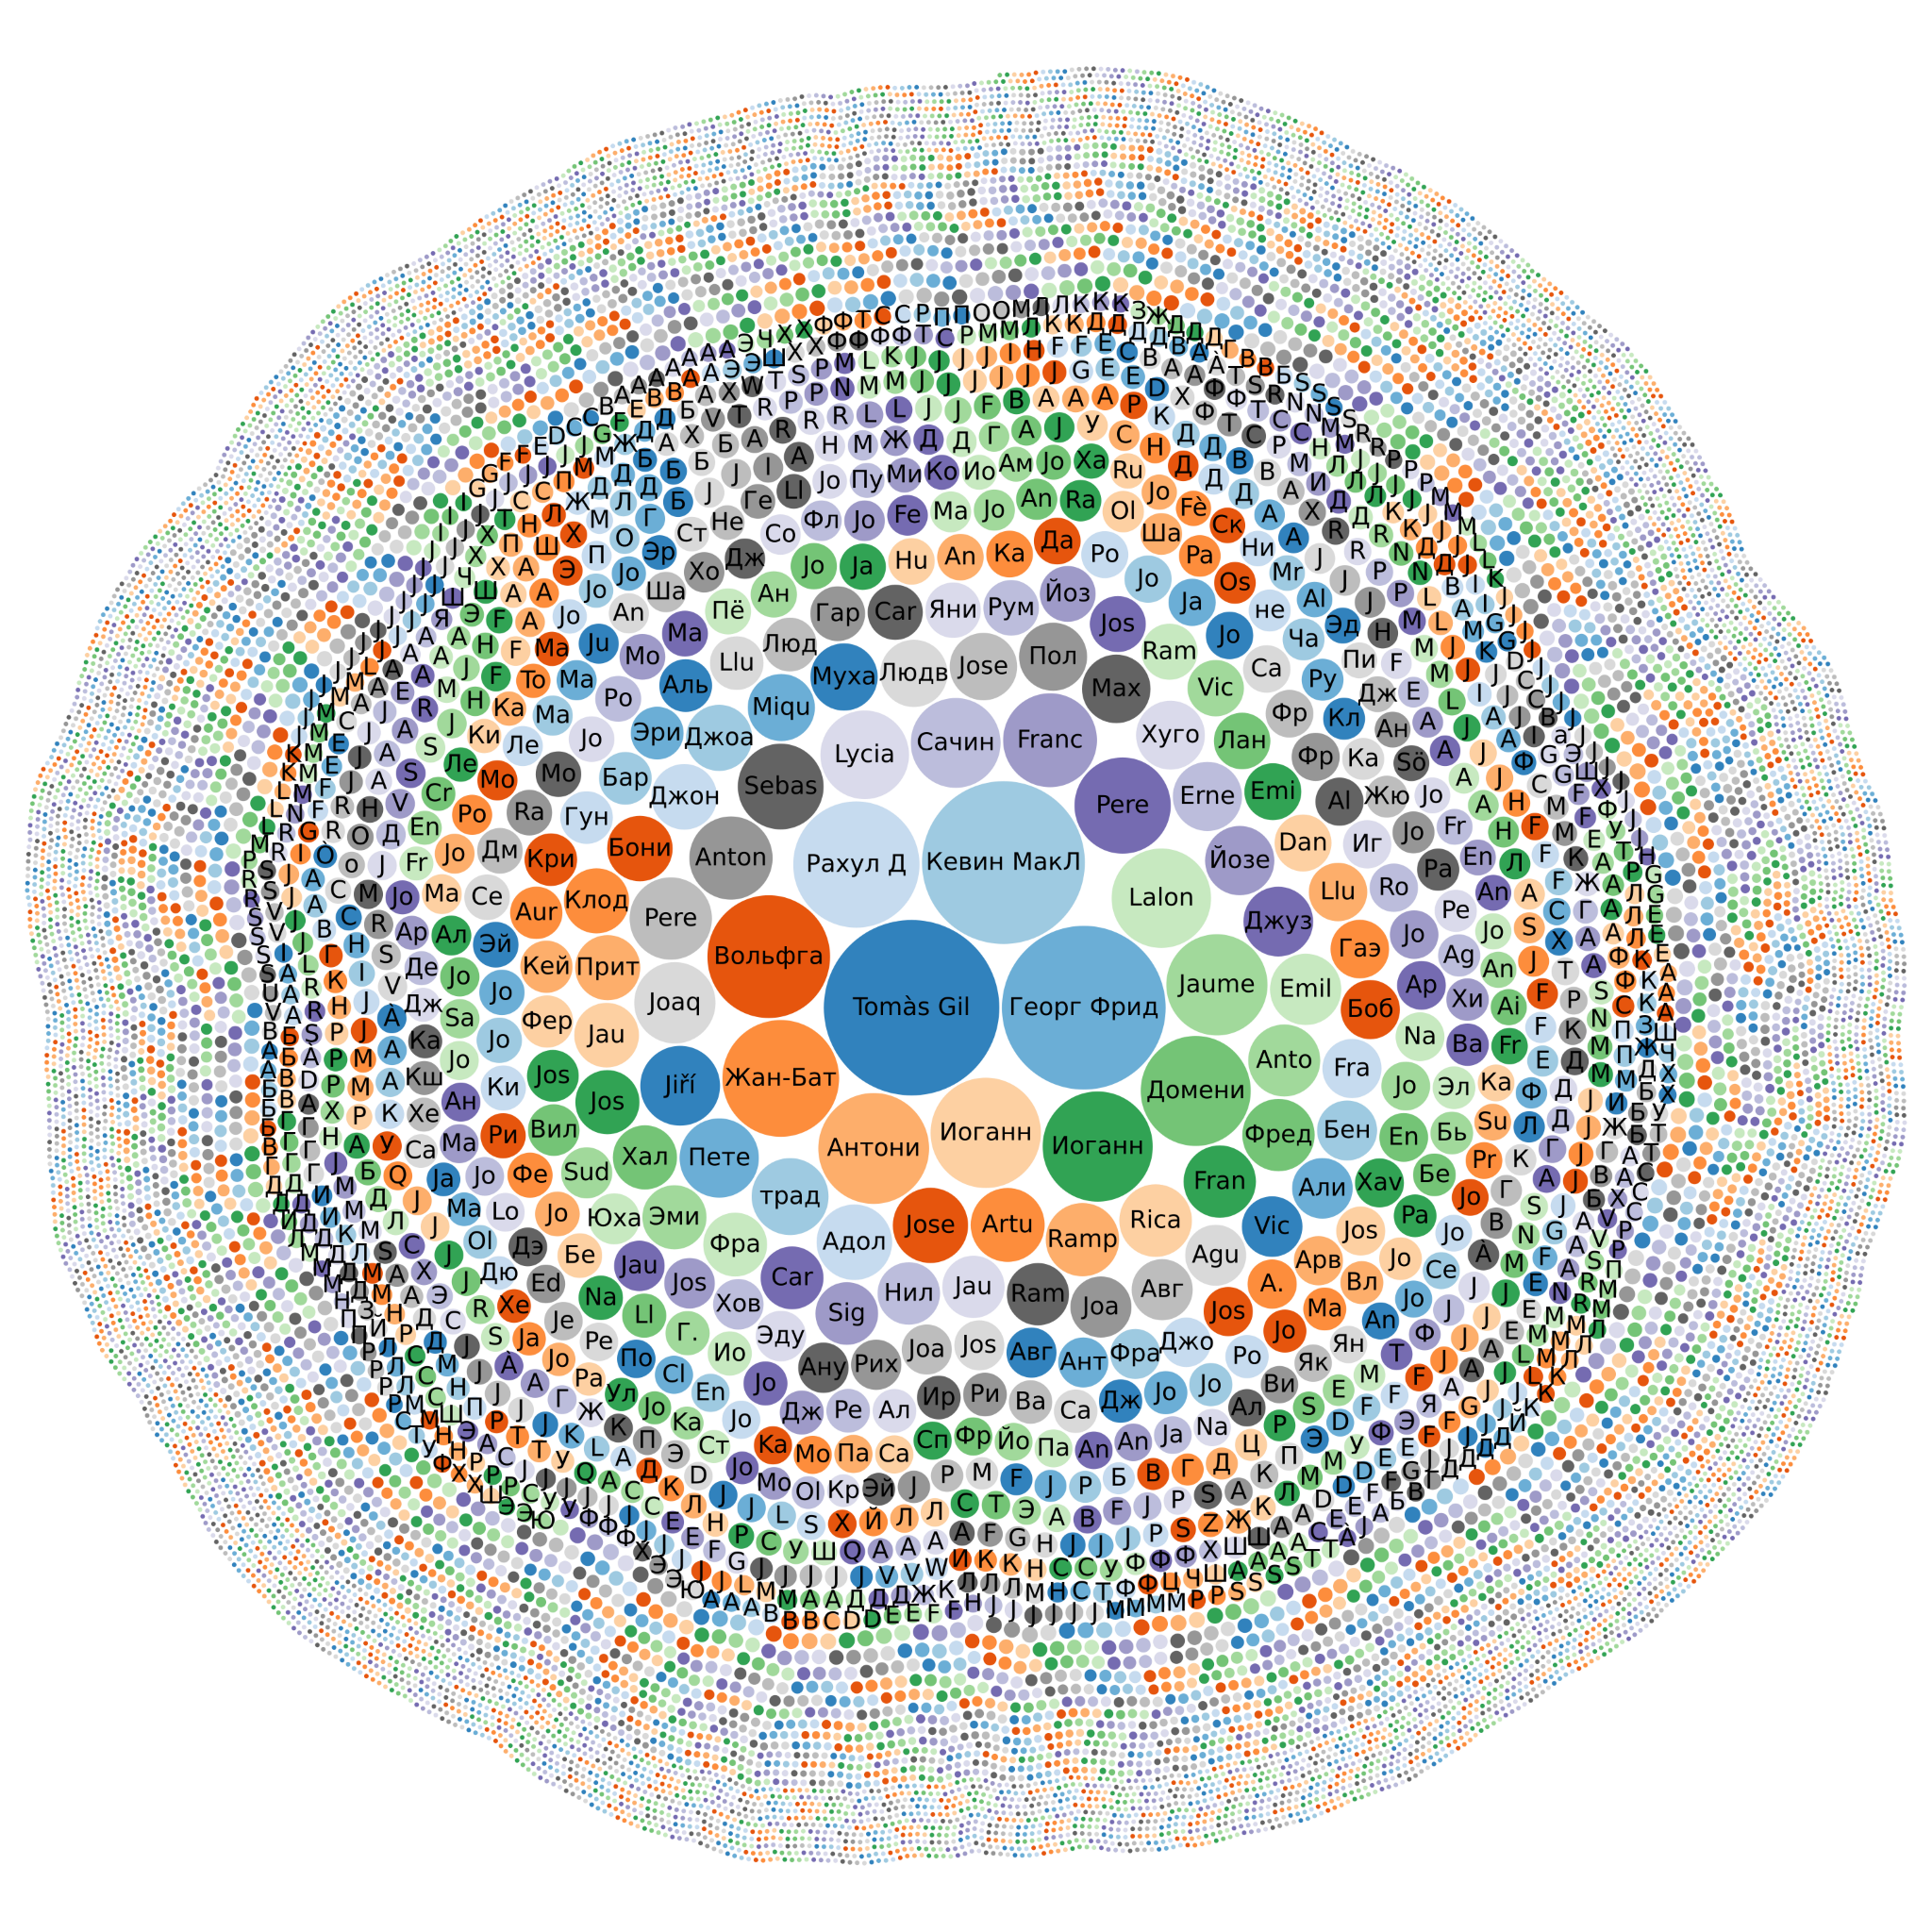
\includegraphics[width=\textwidth]{./chapter/musical_composition/Composer_of_musical_compositions_bubble_diagram.svg.png}
	\caption[Пузырьковая диаграмма композиторов по количеству написанных композиций за 2022 год]{Пузырьковая диаграмма композиторов по количеству написанных композиций за 2022 год}%
	\label{fig:bubbleChart2}%
\end{figure*}
\newpage


\subsection{Заполнение Викиданных}
Для того чтобы получить больше записей при выполнении скрипта для поиска музыкальных лакун в общественном достоянии, было решено заполнить свойство \wdProperty{86}{<<композитор>>} у объектов типа \wdqName{<<музыкальная композиция>>}{207628}.

Построим список всех музыкальных композиций с заполненным свойством \wdProperty{86}{<<композитор>>}.

\begin{lstlisting}[ language=SPARQL,
                    caption={\href{https://w.wiki/52VP}{ список всех музыкальных композиций с заполненным свойством <<композитор>>}\protect\footnotemark},
                    label=lst:Compositions_that_has_a_composer,
                    texcl 
                    ]
#Lists of compositions that has a composer
SELECT ?composition ?compositionLabel ?composer ?composerLabel 
WHERE {
  ?composition wdt:P31 wd:Q207628. # instance of composition
  ?composition wdt:P86 ?composer.  # composition has a composer
  SERVICE wikibase:label {bd:serviceParam wikibase:language "ru".}
}
}
\end{lstlisting}%
\footnotetext{Получено:\num{3965} записей на 2017 год. Ссылка на SPARQL-запрос: \href{https://w.wiki/56Sb}{https://w.wiki/56Sb}.}



\subsection{Упражнения}
\begin{enumerate}
\item Найти список музыкальных композиций, созданных во время эпохи классицизма (XVII—XVIII века).
Свойство: \wdProperty{571}{<<дата создания>>}.
\item Найти композитора, который написал больше симфоний чем остальные.
Свойства: \wdProperty{31}{<<экземпляр>>}, \wdProperty{86}{<<композитор>>}.
\item Построить гистограмму, на которой отображается количество музыкальных композиций группы The Beatles по году публикации.
Свойства: \wdProperty{175}{<<исполнитель>>}, \wdProperty{577}{<<дата публикации>>}.
\end{enumerate}

  \chapter{Национальный парк}
\label{ch:national-park}
Данная статья посвящена исследованию объекта Викиданных <<Национальный парк>>. С помощью SPARQL-запросов, вычисляемых на объектах типа <<национальный парк>> в Викиданных, решены такие задачи: выведен список всех ныне существующих национальных парков, список национальных парков, упорядоченных по дате создания, диаграмма парков, упорядоченных по количеству за разные годы и по странам мира, а так же карта всех национальных парков, построенная на основе географических координат. Кроме того, сделаны выводы по поводу полноты Викиданных по данной теме.


  \chapter{Тематика и социальные сети радиостанций}
\label{ch:radio-station}

Радиостанции --- комплекс устройств и сооружений, служащих для подготовки программ радиовещания. 
Эта глава посвящена исследованию программ радиовещания, 
анализируется объект Викиданных \wdqName {<<вещательная радиостанция>>}{14350} и его свойства. 
Получен список всех радиостанций, описанных в Викиданных. 
С помощью запросов получено количество радиостанций у различных стран, 
определены подклассы радиостанций. 
Найдены радиостанции, вещательные каналы и~СМИ в~СССР и~России, 
выделены группы тематической направленности, 
представлены аккаунты в~социальных сетях.

\section{Число радиостанций по странам}

Получим список всех радиостанций с~указанием страны, к которой они относятся, 
посредством свойства \wdProperty{495}{<<страна происхождения>>}. 
Запрос~\ref{lst:all_radio_stations} вернул около 100 станций, 
что является недостаточным числом для радиовещательных программ всего мира, представленных в Викиданных.

\begin{lstlisting}[ 
    language=SPARQL,
    caption={\href{https://w.wiki/5unA}{Cписок всех радиостанций со свойством <<страна происхождения>>}\protect\footnotemark},
    label=lst:all_radio_stations,
    texcl,
    numbers=none
    ]
# List of radio stations and country
SELECT ?radio ?radioLabel ?countryLabel WHERE
{
  ?radio wdt:P31 wd:Q14350; # instance of radio station
         wdt:P495 ?country. # country of origin
  SERVICE wikibase:label { bd:serviceParam wikibase:language "ru,en" }
}
\end{lstlisting}%
\footnotetext{Получено: 118 результатов на 2024 год. 
              Ссылка на SPARQL-запрос: \href{https://w.wiki/9qag}{https://w.wiki/9qag}.}


Посмотрим количество радиостанций у~разных стран в~запросе~\ref{lst:NStationsCountryP495}.
Суммируем число станций в~переменную \lstinline|?sumRadio| 
с~помощью команды \lstinline|COUNT()| в~строке~2. 
Сгруппируем станции по~странам с~помощью команды \lstinline|GROUP BY| в~строке~7.


        \lstset{escapeinside={(*@}{@*)}}
        \sethlcolor{pink}

\begin{lstlisting}[ 
    language=SPARQL,
    caption={\href{https://w.wiki/9qau}
                  {Количество радиостанций со свойством <<страна происхождения>>
                   по странам}\protect\footnotemark},
    label=lst:NStationsCountryP495,
    xleftmargin=18pt,
    numbers=left,
    ]
# Number of radio stations for each country 
SELECT ((*@\hl{COUNT}@*)(?radio) as (*@\hl{?sumRadio}@*)) ?countryLabel WHERE {
  ?radio wdt:P31 wd:Q14350; # is radio station
         wdt:P495 ?country. # has country of origin
  SERVICE wikibase:label { bd:serviceParam wikibase:language "ru,en" }
}
(*@\hl{GROUP BY}@*) ?countryLabel
ORDER BY DESC (?sumRadio)
\end{lstlisting}%
\footnotetext{Получено: 31 страна с радиостанциями на 2024 год. 
              Ссылка на SPARQL-запрос: \href{https://w.wiki/9qau}{https://w.wiki/9qau}.}

Всего в мире около двухсот стран (смотри главу <<\nameref{ch:country}>> 
на~с.~\pageref{ch:RussiaNotCountryPPS}), 
но запрос~\ref{lst:NStationsCountryP495} нашёл только 31 страну с~радиостанциями. 
По-видимому, свойство \wdProperty{495}{<<страна происхождения>>} больше подходит для~указания 
<<страны происхождения творческого произведения или другого продукта>>, 
что и~указано в~описании этого свойства. 


\begin{margintable}
\caption{Страны с наибольшим числом радиостанций на 2024 год}
\begin{tabular}{|c|c|c|}
\hline
\textnumero & Количество & Страна \\
\hline
1 & 15847 & США \\
2 & 1567 & Мексика \\
3 & 1310 & Канада \\
4 & 980 & Филиппины \\
5 & 824 & Великобритания \\
6 & 734 & Бразилия \\
7 & 584 & Германия \\
8 & 464 & Австралия \\
9 & 427 & Франция \\
10 & 371 & Индия \\
\ldots & \ldots & \ldots \\
23 & 87 & Россия \\
\ldots & \ldots & \ldots \\
32 & 55 & Нидерланды \\
\ldots & \ldots & \ldots \\
\hline
\end{tabular}
\label{tab:number_of_radio_stations}
\end{margintable}


Заменив свойство радиостанций <<страна происхождения>> 
на~свойство <<\wdProperty{17}{государство}>> 
в~строке~4 запроса~\ref{lst:NStationsCountryP17}, 
получим уже больше двухсот стран. 

\begin{lstlisting}[ 
    language=SPARQL,
    caption={\href{https://w.wiki/9qdC}
                  {Количество радиостанций со свойством <<государство>>
                   по~странам}\protect\footnotemark},
    label=lst:NStationsCountryP17,
    xleftmargin=18pt,
    numbers=left,
    ]
# Number of radio stations for each country 
SELECT (COUNT(?radio) as ?sumRadio) ?countryLabel WHERE {
  ?radio wdt:P31 wd:Q14350; # is radio station
         (*@\hl{wdt:P17}@*) ?country.  # from country
  SERVICE wikibase:label { bd:serviceParam wikibase:language "ru,en" }
}
GROUP BY ?countryLabel
ORDER BY DESC (?sumRadio)
\end{lstlisting}%
\footnotetext{Получено: 209 стран с~радиостанциями~на 2024 год. 
              Ссылка на SPARQL-запрос: \href{https://w.wiki/9qdC}{https://w.wiki/9qdC}.}

Из~этих двухсот стран в~табл.~\ref{tab:number_of_radio_stations} 
представлены страны с наибольшим числом станций. 
В Нидерландах по~запросу~\ref{lst:NStationsCountryP495} есть 69 станций 
(в~остальных 30 странах меньше десяти станций), 
а~по~запросу~\ref{lst:NStationsCountryP17}~---  всего 55 радиостанций.



\section{Подклассы радиостанций}

Найдём список подклассов радиостанций и размер подкласса 
с~помощью запроса~\ref{lst:subclasses_of_radio_stations}.

\begin{lstlisting}[ 
    language=SPARQL,
    caption={\href{https://w.wiki/9qej}
                  {Список подклассов радиостанций и размер подклассов}\protect\footnotemark},
    label=lst:subclasses_of_radio_stations,
    xleftmargin=18pt,
    numbers=left,
    ]
# List of radio subclasses and subclass sizes
SELECT ?subRadio ?subRadioLabel (COUNT(?r) AS ?count) WHERE 
{
  ?subRadio wdt:P279* wd:Q14350. # subclass of radio station
  ?r wdt:P31 ?subRadio.          # instance of this subclass
  SERVICE wikibase:label { bd:serviceParam wikibase:language "ru,en" }
}
GROUP BY ?subRadio ?subRadioLabel
ORDER BY DESC(?count)
\end{lstlisting}%

\footnotetext{Получено: 23 подкласса радиостанций на 2024 год. 
              Ссылка на SPARQL-запрос: \href{https://w.wiki/9qej}{https://w.wiki/9qej}.}

Из запроса~\ref{lst:subclasses_of_radio_stations} мы получили встречаемые подклассы радиостанций, что помогло нам понять какой подкласс наиболее актуален. 

\marginnote[1\baselineskip]{%
        \label{question:radio}
        \MarginQuestion
        Запрос~\ref{lst:subclasses_of_radio_stations} написан с ошибкой, потому что в результате поиска подклассов радиостанций мы получаем сами \wdqName{<<вещательные радиостанции>>}{14350} . Так почему в списке подклассов мы получаем сами радиостанции? И что необходимо исправить в запросе~\ref{lst:subclasses_of_radio_stations}, чтобы сам класс не попадал в свои подклассы? 
        
        См. ответ на~с.~\pageref{answer:radio_station}.
}

\todoVlad{
Егор, Вы мне задали правильный вопрос, почему в списке подклассов радиостанции мы 
опять получаем радиостанцию, причём это самый большой подкласс, содержит около 30 тыс. объектов.\\

\vspace{12pt}
Напишите на полях этот вопрос
(см. как это сделано в главе про музыку у Владимира, 
ищите команду 
{\textbackslash}MarginQuestion 
 в коде его главе, она отрисовывает настольную лампу).\\ 
И дополните этот вопрос просьбой к читателю, 
чтобы он исправил запрос~\ref{lst:subclasses_of_radio_stations} так, 
чтобы сам класс не попадал в свои подклассы.\\ 
Подсказка: нужно использовать квантификатор +, а не звёздочку *.\\

\vspace{12pt}
И второе, Егор, в разделе <<Ответы>> в конце книги (файл answers) 
напишите ответ на этот вопрос и на эту просьбу (напишите правильный запрос).\\ 
Должны быть перекрёстные ссылки: с вопроса на ответ и обратно. 
Посмотрите, как это сделано у Владимира. }
\answerVlad{Ответ: сделано }




\newpage
\section{Отечественные радиостанции, СМИ и вещательные каналы: UNION против VALUES}

Найдём радиостанции, вещательные каналы и СМИ в СССР и России 
с~помощью запроса~\ref{lst:radioRussiaUNION}. 
Радиостанции не повторяются благодаря команде \lstinline|DISTINCT| в~строке~2. 

Запрос получился достаточно громоздкий из-за использования команды \lstinline|UNION|. 
Перепишем скрипт с~использованием команды \lstinline|VALUES|, 
объединяющей значения (объекты Викиданных) в массив. 
Обычно код с командой \lstinline|VALUES| становится компактнее. 
Запрос~\ref{lst:radioRussiaVALUES} получился короче на одну строку, 
но кажется более простым для понимания, поскольку вся соль скрипта заключена 
в строках 7 и 8. 


\begin{lstlisting}[ 
    language=SPARQL,
    caption={\href{https://w.wiki/9qst}{Список радиостанций, вещательных каналов и СМИ в России, и СССР}\protect\footnotemark},
    label=lst:radioRussiaUNION,
    xleftmargin=18pt,
    numbers=left,
    ]
# List of radio stations, broadcasting and mass media in Russia 
SELECT (*@\hl{DISTINCT}@*) ?radio ?radioLabel WHERE
{
  {?radio wdt:P31 wd:Q14350}    UNION # is radio station OR
  {?radio wdt:P31 wd:Q15265344} UNION # is broadcasting OR
  {?radio wdt:P31 wd:Q11033}          # is mass media
    
  {?radio wdt:P17 wd:Q15180} UNION    # in USSR OR
  {?radio wdt:P17 wd:Q159}            # in Russia
  SERVICE wikibase:label { bd:serviceParam wikibase:language "ru,en" }
}
\end{lstlisting}%
\footnotetext{Получено: 121 радиостанция на 2024 год. 
              Ссылка на SPARQL-запрос: \href{https://w.wiki/9qst}{https://w.wiki/9qst}. }


\begin{lstlisting}[ 
    language=SPARQL,
    caption={\href{https://w.wiki/9quA}{Радиостанции, вещательные каналы и СМИ по России, и по СССР}\protect\footnotemark},
    label=lst:radioRussiaVALUES,
    xleftmargin=18pt,
    numbers=left,
    ]
# List of radio stations, broadcasting and mass media in Russia 
SELECT DISTINCT ?radio ?radioLabel ?mediaTypeLabel ?countryLabel WHERE
{           # radio station, broadcasting, mass media
  VALUES ?mediaType {wd:Q14350 wd:Q15265344 wd:Q11033}
  VALUES ?country {wd:Q15180 wd:Q159} 
              # Soviet Union, Russia
  ?radio wdt:P31 ?mediaType; # is one of mass media
         wdt:P17 ?country.   # related to Soviet Union or Russia
  SERVICE wikibase:label { bd:serviceParam wikibase:language "ru,en" }
}
\end{lstlisting}%
\footnotetext{Получено: 129 радиостанций на 2024 год. 
              Ссылка на SPARQL-запрос: \href{https://w.wiki/9quA}{https://w.wiki/9quA}. }


Одним из преимуществ такого подхода с использованием команды \lstinline|VALUES| 
стало то, что мы можем воспользоваться именами массивов \lstinline|?mediaType| и \lstinline|?country|, 
чтобы вывести на печать вид медиа и страну 
(\lstinline|?mediaTypeLabel| и \lstinline|?countryLabel|) 
в~строке~2 запроса~\ref{lst:radioRussiaVALUES}.

\marginnote[1\baselineskip]{%
        \label{question:radio2}
        \MarginQuestion
	 В выводе запроса~\ref{lst:radioRussiaUNION} мы можем видеть 121 радиостанцию, а в запросе~\ref{lst:radioRussiaVALUES} 129 радиостанций.
        Исходя из результатов можно задаться вопросом: почему имеются различия в запросах, если они выполняют идентичную задачу? 
        
        См. ответ на~с.~\pageref{answer:radio_station2}.
}
 



\todoVlad{
Егор, в запросе~\ref{lst:radioRussiaUNION} с~UNION было 120 станций. 
А после замены на VALUES в запросе~\ref{lst:radioRussiaVALUES}
стало 128 станций.\\
Напишите на поля вопрос об этом (с лампочкой).\\

\vspace{12pt}
В ответе в главе <<Ответы>> попробуйте это объяснить. 
Чтобы понять, в чём дело: найдите примеры станций, которые появляются во втором случае, 
посмотрите на их свойства на Викиданных.}
\answerVlad{Ответ: сделано }





\newpage
\section{Темы отечественных радиостанций и конкатенация строк}

Попробуем понять, какие темы представлены на радиостанциях, СМИ и~вещательных каналах в~СССР и~России 
с~помощью запроса~\ref{lst:SubjRadio}. 

Главные темы радиостанций и других объектов задаются свойством \wdProperty{921}{<<основная тема>>}. 
У~одной станции может быть указано несколько тем, 
см. столбец <<Тема (mainSubject)>> в~табл.~\ref{tab:CONCAT}. 
В этой таблице приведены примеры главных тем для <<Радио Звезда>> и <<Марий Эл Радио>>.

Функция \lstinline|GROUP_CONCAT| (строка~3 запроса~\ref{lst:SubjRadio}) 
объединяет (конкатенирует) строки \lstinline|?subjName|, <<склеивая>> их разделителем, 
здесь~--- запятой с пробелом. 


\begin{margintable}
\centering
\caption{Две радиостанции с примером использования функции \lstinline|GROUP\_CONCAT|, 
         результат записан в переменную ?mainSubject}
%\begin{tabular}{|p{14em}|p{10em}|p{10em}|}
\begin{tabular}{|p{64pt}|p{62pt}|p{96pt}|}
\hline
Объект (radio) & Метка (radioName) & Тема (mainSubject) \\
\hline
\wdqName{Radio Zvezda}{4387399} & Радио Звезда & война, политика, экономика, вооружённые силы, новости, patriot \\
\hline
\wdqName{Mari~El Radio}{30909585}
    \href{Q30909585} & Марий Эл Радио & музыка, комедия, интервью \\
\hline
\end{tabular}
\label{tab:CONCAT}
\end{margintable}


\begin{lstlisting}[ 
    language=SPARQL,
    caption={\href{https://w.wiki/9qwk}
                  {Список тематик радиостанций, СМИ и вещательных каналов}\protect\footnotemark},
    label=lst:SubjRadio,
    xleftmargin=18pt,
    numbers=left,
    ]
# List of the main topics of radio stations, media and mass media
SELECT ?radio ?radioName
       ((*@\hl{GROUP\_CONCAT}@*)(DISTINCT ?subjName;separator=", ") AS ?mainSubjects) WHERE 
{           # radio station, broadcasting, mass media
  VALUES ?mediaType {wd:Q14350 wd:Q15265344 wd:Q11033}
  VALUES ?country {wd:Q15180 wd:Q159} 
              # Soviet Union, Russia
  
  ?radio wdt:P31 ?mediaType; # is one of mass media
         wdt:P17 ?country;   # in country  
         wdt:P921 ?subj.     # has main topic
  
  SERVICE wikibase:label { bd:serviceParam wikibase:language "ru,en".
                           ?radio rdfs:label ?radioName.
                           ?subj  rdfs:label ?subjName. }
} GROUP BY ?radio ?radioName
\end{lstlisting}%
\footnotetext{Получено: 73 тематические группы на 2024 год. 
              Ссылка на SPARQL-запрос: \href{https://w.wiki/9qwk}{https://w.wiki/9qwk}.}

\marginnote[1\baselineskip]{%
        \label{question:radio3}
        \MarginQuestion
	 В запросе~\ref{lst:SubjRadio} вёлся поиск тематик радиостанций, СМИ и вещательных каналов. Далее была построена таблица~\ref{tab:number_of_topics}. Возможно ли создать граф с вершинами двух типов? Первый тип вершин: вершина соответствует ровно одной главной теме, например, «медицина» или «здоровье», или «юмор».  Второй тип вершин: вершина — это радиостанция. Ребро между радиостанцией и какой-либо темой отрисовывается, если эта тема указана в свойствах объекта этого радио на сайте Викиданных.
}


\todoVlad{
Егор, напишите на поля вопрос (с лампочкой) о том, чтобы читатель построил такой запрос, 
чтобы можно было создать граф с вершинами двух типов:\\ 
(1) вершина соответствует ровно одной главной теме, например, <<медицина>> или <<здоровье>>, или <<юмор>>.\\
(2) вершина~--- это радиостанция. 
Ребро между радиостанцией и какой-либо темой отрисовывается, 
если эта тема указана в свойствах объекта этого радио на сайте Викиданных. 

\vspace{12pt}
Ответ в главе <<Ответы>> не требуется.}
\answerVlad{Ответ: сделано }





\begin{margintable}
\caption{Количество тематик у радиостанций, СМИ и вещательных каналов по убыванию на 2023 год}
\begin{tabular}{|c|c|}
\hline
Количество тематик по & Название тематики \\
 \wdProperty{921}{<<основная тема>>} & \\
\hline
44 & музыка \\
5 & поп-музыка \\
5 & рок \\
3 & TopHit \\
3 & хип-хоп \\
3 & молодёжная музыка \\
3 & джаз \\
\hline
30 & новости \\
15 & политика \\
7 & экономика \\
5 & пропаганда \\
5 & авария \\
5 & проект \\
2 & политическая система России \\
\hline
9 & ток-шоу \\
5 & спорт \\
3 & шутка \\
2 & юмор \\
2 & комедия \\
2 & художественная литература \\
3 & спектакль \\
\hline
\end{tabular}
\label{tab:number_of_topics}
\end{margintable}

Таблица~\ref{tab:number_of_topics} даёт нам представление того, 
какие темы более популярны на радиостациях, а~именно:
\wdqName{музыка}{638}, 
\wdqName{новости}{38926} и \wdqName{политика}{7163}.


\todoVlad{
    Егор, получилась отличная таблица. Добавьте к ней следующий запрос (вместе с листингом), 
    чтобы объяснить откуда она появилась:
\url{https://w.wiki/9rLD}.\\
Обновите данные в таблице в соответствии с этим запросом, возможно где-то цифры немного изменились. 

\vspace{12pt}
Закомментируйте строки 5 и 9 в этом листинге, связанные с Россией, и подсчитайте 
то же самое по всем странам мира. 
Добавьте в эту таблицу последний (третий) столбец с числами тематик по всему миру.\\ 
Поменяйте местами первый и второй столбец. То есть порядок столбцов будет такой:
(1) Название, (2) в России, (3) в мире. 

\vspace{12pt}
Сейчас в таблице темы разделены на три логических блока. Это хорошая идея. 
Здесь текстом напишите пояснение - что это за блоки, какие темы являются лидерами в блоке, 
на скольких радиостанциях есть такие темы. 

\vspace{12pt}
Не нужно писать <<Данная таблица>>. Пишите с помощью команды ref - 
также как Вы это делаете при ссылках на запросы или рисунку. Т.е. будет:
<<В табл. N.N ...>>
}
\answerVlad{Ответ: после комментирования строк, результат изменился незначительно (на 9, 3 и меньше).  Может быть я что-то не так сделал, но это маловероятно }











\newpage
\section{Радиостанции, СМИ и вещательные каналы в социальных сетях}

Данный запрос~\ref{lst:socialNetBubbles} находит аккаунты радиостанций, СМИ и вещательных каналов в социальных сетях.

\begin{lstlisting}[ 
    language=SPARQL,
    caption={\href{https://w.wiki/6fKb}{Аккаунты радиостанций, СМИ и вещательных каналов в социальных сетях}\protect\footnotemark},
    label=lst:socialNetBubbles,
    xleftmargin=18pt,
    numbers=left,
    ]
# Counts the number of radios with social media accounts
#defaultView:BubbleChart
SELECT ?netID ?netIDLabel ?netRelation (COUNT(?network) as ?sumNetwork)
WHERE
{                  # Facebook, Instagram, Telegram, Twitter, VK, YouTube, Zen, SoundCloud, Google ID, Odnoklassniki, Rutube, Spotify
  VALUES ?netRelation {wdt:P2013 wdt:P2003 wdt:P3789 wdt:P2002 wdt:P3185 wdt:P2397 wdt:P8816 wdt:P3040 wdt:P2847 wdt:P5163 wdt:P10152 wdt:P5916}
  
  ?radio wdt:P31 wd:Q14350; # instance of radio station
         wdt:P17 wd:Q159;   # radio from Russia
         ?netRelation ?network. # has social network page

  ?netID wikibase:directClaim ?netRelation.
  
  SERVICE wikibase:label {bd:serviceParam wikibase:language "en"}
} GROUP BY ?netID ?netIDLabel ?netRelation 
ORDER BY DESC(?sumNetwork)\end{lstlisting}%

\footnotetext{Получено: \num{12} результатов на 2023 год. Ссылка на SPARQL-запрос: \href{https://w.wiki/6fKb}{https://w.wiki/6fKb}. }

Объясним строку 12 \lstinline|?netID wikibase:directClaim ?netRelation| и необходимость использования предиката wikibase:directClaim в запросе~\ref{lst:socialNetBubbles}.

Для этого нужно начать с объяснения того, что радиостанции соответствует объект и страница на Викиданных. На этой странице есть подраздел Идентификаторы (Identifiers). В этом подразделе перечислены, в том числе, социальные сети, в которых зарегистрирован объект (здесь радиостанция). Два следующих утверждених из запроса выше (на примере ВКонтакте, которому соответствует идентификатор-свойство P3185):

\begin{lstlisting}
# VALUES ?netRelation ... wdt:P3185
# ?radio ... ?netRelation ?network. \# has social network page
\end{lstlisting}

мы получаем ?netRelation для каждой радиостанции, счетчик ?sumNetwork (здесь для ВКонтакте) увеличивается на один.

Проблема в том, что мы не можем получить имя \lstinline|?netRelationLabel|, поскольку конструкция \lstinline|SERVICE wikibase| не работает для свойств, а только для объектов. Нам помогает свойство \lstinline|wikibase:directClaim|, которое возвращает имя \lstinline|?netID| по свойству \lstinline|?netRelation|.


Пузырьковая диаграмма~\ref{fig:radio_station_acc} построенная запросом~\ref{lst:socialNetBubbles}, показывает количество аккаунтов СМИ и радиостанций в социальных сетях. То есть на рисунке показаны социальные сети, размер круга пропорционален количеству зарегистрированных в них аккаунтов СМИ и радиостанций.

Популярными социальными сетями среди радиостанций, СМИ и вещательных каналов в России на 2024 год стали: 
ВКонтакте~--- 28 аккаунтов; 
Instagram~--- 26 аккаунтов; 
Facebook~--- 25 аккаунтов; 
YouTube~--- 24 аккаунта; 
Twitter~--- 21 аккаунт; 
Telegram~--- 20 аккаунтов. 
Таким образом, самой популярной социальной сетью для СМИ в России стал ВКонтакте.

Следующим шагом будет проведено сравнение количества аккаунтов радиостанций, СМИ и вещательных каналов России и всех стран в социальных сетях. Для этого необходимо закомментировать строку 9~\lstline|wdt:P17 wd:Q159| в запросе~\ref{lst:socialNetBubbles}, которая нужна нам для поиска в России.  Аналогично будет построена пузырьковая диаграмма для всех стран, которую построил запрос~\ref{lst:socialNetBubbles} с закомментированной строкой, о которой говорилось ранее. 

Популярными социальными сетями среди радиостанций, СМИ и вещательных каналов во всех странах на 2024 год стали:
Twitter~---4835 аккаунтов;
Facebook~---2044 аккаунтов;
Instagram~---1514 аккаунтов;
Youtube~---397 аккаунтов;
Telegram~---51 аккаунт;
Вконтакте~---44 аккаунта.
Таким образом, самой популярной социальной сетью для СМИ всех стран стал Twitter.

Глядя на результаты двух диаграмм можно сделать вывод о том, что в шестерка популярных социальных сетей осталась почти неизменной, изменились только позиции. Таким образом во второй диаграмме~\ref{fig:radio_station_acc_all_countries}  верхние строчки заняли социальные сети, имеющие большую популярность во всем мире. Социальные сети, которые разработаны в России заняли места ниже в этой шестерке. 



\index{График!Sunburst diagram}
\begin{marginfigure}[1\baselineskip]
{\includegraphics[width=1\linewidth]{chapter/radio_station/Number_of_social_media_accounts_2.png}}
\vspace{-7pt}
\caption{Пузырьковая диаграмма популярности социальных сетей по числу в них аккаунтов радиостанций, СМИ и вещательных каналов на 2024 год}%
\label{fig:radio_station_acc}
\end{marginfigure}

\index{График!Sunburst diagram}
\begin{marginfigure}[1\baselineskip]
{\includegraphics[width=1\linewidth]{chapter/radio_station/Number_of_social_media_accounts_in_all_countries.png}}
\vspace{-7pt}
\caption{Пузырьковая диаграмма популярности социальных сетей по числу в них аккаунтов радиостанций, СМИ и вещательных каналов во всех странах на 2024 год}%
\label{fig:radio_station_acc_all_countries}
\end{marginfigure}


\todoVlad{
Егор, сделайте второй рисунок, 
закомментировав строчку в~запросе~\ref{lst:socialNetBubbles} 
о принадлежности радио к России.\\
Добавьте этот второй рисунок сюда. Напишите словами о разнице между этими двумя диаграммами: про число аккаунтов отечественных радиостанций в соцсетях относительно числа аккаунтов радио всего мира.\\
Второй листинг делать не надо, поскольку он отличается только одной строчкой - 
достаточно в тексте написать - номер строки, которую комментируете.

\vspace{12pt}
Не забудьте при создании картинки отредактировать SVG-файл, чтобы был крупный шрифт для надписей внутри кружков.
}
\answerVlad{Ответ: сделано }

}

\iffalse
\setchapterimage[6cm]{chapter/operating_system/logo.png}
\setchapterpreamble[u]{\margintoc}
\chapter[line 1 line 2]{Programming languages for operating systems}
\labch{operating-sysmets}

\section{Annotation}
The chapter explores the object of the <<operating system>> and its properties. The following problems were solved in the paper with the help of SPARQL queries: finding instances of the object <<operating system>>, building a list of operating systems (OS) by base, by creation time, by programming language, in which the OS was written. Also a histogram is constructed, it shows the number of programs written in some programming language, and the proportion of how many of them work for some OS. A lot of software does not specify the programming language on which it was developed. The property <<programming language>> was added to several objects to improve the results.

\section{Instances of the object "operating system"}

Let's build a list of all the operating systems.

\begin{lstlisting}[ language=SPARQL, 
caption={List of operating systems\\\hspace{\textwidth} 
SPARQL query \num{510} results (January 2018), \num{1086} results (September 2020).
SPARQL query: \href{https://w.wiki/nDb}{https://w.wiki/nDb}
},
label=lst:os-list,
texcl 
]
#List of `instances of` "operating system" 
SELECT ?os ?osLabel
WHERE
{
	?os wdt:P31 wd:Q9135.
	SERVICE wikibase:label { bd:serviceParam wikibase:language "en" }
}
}
\end{lstlisting}

[+]> The most complete and detailed operating systems on Wikidata are: Linux, Windows, Windows 8

[-]> Almost empty and less informative operating systems are: SPIN, JavaOS, Atari TOS, Xubuntu

According to ProWD the only one Russian operating system on Wikidata is Miraculix, which has 7 properties. The leaders in terms of the number of properties (24 properties) among operating systems around the world are Microsoft Windows and Windows 8.

\section{List of operating systems by base}

\begin{lstlisting}[ language=SPARQL, 
caption={List of operating systems by base\\\hspace{\textwidth}
SPARQL query \num{159} results (January 2018), \num{118} results (September 2020).
SPARQL query: \href{https://w.wiki/nDc}{https://w.wiki/nDc}
},
label=lst:os-by-base,
texcl 
]
SELECT ?osLabel ?baseLabel
WHERE
{
	?os wdt:P31 wd:Q9135. # inctance of operating system
	?os wdt:P144 ?base. # os is base for 
	SERVICE wikibase:label { bd:serviceParam wikibase:language "en" }
}
GROUP BY ?osLabel ?baseLabel
\end{lstlisting}

\section{List of operating systems by creation time}


\begin{lstlisting}[ language=SPARQL, 
caption={List of operating systems by creation time\\\hspace{\textwidth}
SPARQL query \num{298} results (January 2018), \num{238} results (September 2020).
SPARQL query: \href{https://w.wiki/nDf}{https://w.wiki/nDf}
},
label=lst:os-creation-time,
texcl 
]
#defaultView:Timeline
SELECT ?osLabel ?time
WHERE
{
	?os wdt:P31 wd:Q9135. # inctance of operating system
	?os wdt:P571 ?time. # created at
	SERVICE wikibase:label { bd:serviceParam wikibase:language "en" }
}
GROUP BY ?osLabel ?time
ORDER BY DESC(?time)
\end{lstlisting}

\section{Count of operating systems by programming language}

\begin{lstlisting}[ language=SPARQL, 
caption={Count of operating systems by programming language\\\hspace{\textwidth}
SPARQL query \num{35} results (January 2018), \num{37} results (September 2020).
SPARQL query: \href{https://w.wiki/nDh}{https://w.wiki/nDh}
},
label=lst:prog-lang-count,
texcl 
]
#defaultView:BarChart
SELECT ?lang (count(*) as ?count)
WHERE 
{
	?os wdt:P31 wd:Q9135.
	?os wdt:P277 ?langObj .
	OPTIONAL {
		?langObj rdfs:label ?lang
		filter (lang(?lang) = "en")
	}
}
GROUP BY ?lang
ORDER BY DESC(?count) ASC(?lang)
\end{lstlisting}

The query shows (only on the basis of the completed wikis, so it's not a fact that it's true) that the OS is predominantly written in Assembler language, which is certainly true, because it is the fastest, yet convenient programming language. On the second and third places are C and C++, which are not the worst analogue, because in spite of its "slowness", they are the most convenient and simple programming languages.

\subsection{The programming languages used to write the operating system}

It is also interesting to look at the results of this query in the form of a graph, it is also perfectly visible on it how many objects simply have an empty field "programming language".

\begin{lstlisting}[ language=SPARQL, 
caption={The programming languages used to write the operating system\\\hspace{\textwidth}
SPARQL query \num{533} results (March 2017), \num{1117} results (September 2020)
SPARQL query: \href{https://w.wiki/eLH}{https://w.wiki/eLH}
},
label=lst:lang-used-to-os,
texcl 
]
#defaultView:BarChart
SELECT ?lang (count(*) as ?count)
WHERE 
{
	?os wdt:P31 wd:Q9135.
	?os wdt:P277 ?langObj .
	OPTIONAL {
		?langObj rdfs:label ?lang
		filter (lang(?lang) = "en")
	}
}
GROUP BY ?lang
ORDER BY DESC(?count) ASC(?lang)
\end{lstlisting}

If you look at the same query, but with such a restriction that at least the number of operating systems written in the language is at least 2, you can see a significant difference with the result of the previous query.


\begin{lstlisting}[ language=SPARQL, 
caption={Graph of languages used to create operating systems\\\hspace{\textwidth}
SPARQL query \num{118} results (September 2020)
SPARQL query: \href{https://w.wiki/nDm}{https://w.wiki/nDm}
},
label=lst:graph-os-by-lang,
texcl 
]
#defaultView:Graph
SELECT ?os ?osLabel ?language ?languageLabel
WHERE
{
	{
		SELECT ?language ?languageLabel
		WHERE {
			?os wdt:P31 wd:Q9135. # os is os
			?os wdt:P277 ?language. # os written by language
			SERVICE wikibase:label { bd:serviceParam wikibase:language "en" }
		} 
		Group by ?language ?languageLabel 
		Having (Count(?os) > 1) # get laguages which has more than one written os
	}
	?os wdt:P31 wd:Q9135. # os is os
	?os wdt:P277 ?language. # os written by language
	SERVICE wikibase:label { bd:serviceParam wikibase:language "en" }
}
\end{lstlisting}
\setchapterpreamble[u]{\margintoc}
\chapter{Chapter's title}
\labch{the-label-of-your-title5}

\section{The section title}



%\fi %eo iffalse2
\chapter{Военные корабли и их операторы}
\label{ch:ships-chapter}

Глава посвящена отечественным и зарубежным кораблям. Они могут иметь как военное, так и гражданское назначение. Гражданские суда используются в грузоперевозках, рыболовстве, туризме, разведке полезных ископаемых, спасательных работах, а также в спортивных, культурных и других целях. Для хранения информации о судах и других объектах ведутся базы знаний. Одной из таких баз знаний являются Викиданные. В этой главе изучены хранимык в Викиданных объекты кораблей и проведена оценке качества и полноты их описания.


\begin{marginfigure}[0.0cm]
  {
    \setlength{\fboxsep}{0pt}%
    \setlength{\fboxrule}{1pt}%
    \fcolorbox{gray}{gray}{\includegraphics{chapter/ship/Russian_ships_topic_imbalance.png}}
  }
  \caption{
    График равномерности заполнения по числу свойств объекта Викиданных \href{https://www.wikidata.org/wiki/Q11446}{корабль (Q11446)}, коэффициент Джини равен 0.239. Данные получены с помощью сервиса ProWD.id, 2020 год. График и коэффициент Джини показывают низкую равномерность заполнения свойств.
    }%
    \label{fig:prowd_ships-unbalanced}%
  \end{marginfigure}

\section{Список кораблей}

\marginnote{
\href{https://www.wikidata.org/wiki/Q11446}{Корабль (Q11446)} -- это крупное морское судно.

Исследуемые свойства:
\begin{itemize}
  \item\href{https://www.wikidata.org/wiki/Property:P31}{Экземпляр (P31)}.
  \item\href{https://www.wikidata.org/wiki/Property:P137}{Оператор (P137)}.
  \item\href{https://www.wikidata.org/wiki/Property:P17}{Государство (P17)}.
  \item\href{https://www.wikidata.org/wiki/Property:P607}{Конфликт (P607)}
\end{itemize}
}

Построим список всех кораблей (см. листинг \ref{lst:ships_ru}).

\begin{lstlisting}[ language=SPARQL, caption={{\href{https://w.wiki/koL}{Список кораблей}}\protect\footnotemark}, label=lst:ships_ru, ]
#List of ship
SELECT ?ship ?shipLabel
WHERE
{
  ?ship wdt:P31 wd:Q11446. # instance of ship
  SERVICE wikibase:label { bd:serviceParam wikibase:language "ru". }
}
\end{lstlisting}
\footnotetext{Найдено \num{19820} кораблей в 2017 г. и \num{50681} в 2020 г. Ссылка на SPARQL-запрос: \href{https://w.wiki/koL}{https://w.wiki/koL}. }

По данным ProWD больше всего свойств (34) имеет \href{https://www.wikidata.org/wiki/Q281147}{ледокол Красин}\cite{ProWD_ru_ships}.

Составим список кораблей, операторы которых находятся или находились в России, СССР или Российской империи (см. листинг \ref{lst:ships_with_ru_op}).

\begin{lstlisting}[ language=SPARQL, caption={\href{https://w.wiki/koN}{Cписок кораблей, операторы которых находятся или находились в России, СССР или Российской Империи}}, label=lst:ships_with_ru_op ]
#List of ship from Russia, Soviet Union and Russian Empire
SELECT ?ship ?shipLabel
WHERE
{
  ?ship wdt:P31 wd:Q11446. # instance of ship
                                    # ships belongs to:
  { ?ship wdt:P137/wdt:P17 wd:Q34266 } UNION  # Russian Empire
  { ?ship wdt:P137/wdt:P17 wd:Q15180 } UNION  # Soviet Union
  { ?ship wdt:P137/wdt:P17 wd:Q159 }.         # Russia
  SERVICE wikibase:label { bd:serviceParam wikibase:language "ru". }
}
\end{lstlisting}
\footnotetext{Найдено 579 кораблей в 2020 г. Ссылка на SPARQL-запрос: \href{https://w.wiki/koN}{https://w.wiki/koN}.}

% \section{Плохие и хорошие примеры}

% Хорошие примеры объектов кораблей на сайте Викиданных: \href{https://www.wikidata.org/wiki/Q613128}{SMS Moltke}, \href{https://www.wikidata.org/wiki/Q596282}{HMS Hermes}, \href{https://www.wikidata.org/wiki/Q596282}{HMS Barham}.

% Плохими примерами объектов кораблей на сайте Викиданных были: \href{https://www.wikidata.org/wiki/Q4264229}{Лихой}, \href{https://www.wikidata.org/wiki/Q18816894}{Николай Вилков}, \href{https://www.wikidata.org/wiki/Q4528362}{Щ-310}.

\section{Полнота Викиданных}

Поиск точного количества кораблей в мире — трудная задача. Ведь данные о некоторых из них являются совершенно секретными, какие-то же — это частные судна и информации о них тоже нет. Предположим, что общее число кораблей равно \num{1641690}, как указано в базе данных судов\cite{FleetMon}. На 2021 год было найдено только \num{71206} записей, что составило только 4,3\% от общего числа кораблей. См. листинг \ref{lst:all_ships_en}.


\begin{lstlisting}[ language=SPARQL, caption={\href{https://w.wiki/koU}{Список кораблей на английском}}, label=lst:all_ships_en ]
#List of ships in English
SELECT ?ship ?shipLabel
WHERE
{
  ?ship wdt:P31 wd:Q11446.
  SERVICE wikibase:label { bd:serviceParam wikibase:language "en". }
}
\end{lstlisting}
\footnotetext{Ссылка на SPARQL-запрос: \href{https://w.wiki/koU}{https://w.wiki/koU}.}

Что касается российских кораблей, актуальный список корабельного состава Военно-морского флота Российской Федерации России на 16 октября 2017 г., содержит 72 подводные лодки, а также 211 боевых кораблей и катеров\cite{RussianShips}, При этом запрос в листинге \ref{lst:all_ru_ships} находит всего 25 записей (0.09\%).

\begin{lstlisting}[ language=SPARQL, caption={\href{https://w.wiki/koS}{Cписок кораблей, операторы которых находятся или находились в России, СССР или Российской Империи}}, label=lst:all_ru_ships ]
#List of ship from Russia, Soviet Union and Russian Empire
SELECT ?ship ?shipLabel
WHERE
{
  ?ship wdt:P31 wd:Q11446. # instance of ship
                                     # ships belongs to:
  { ?ship wdt:P137/wdt:P17 wd:Q34266 } UNION  # Russian Empire
  { ?ship wdt:P137/wdt:P17 wd:Q15180 } UNION  # Soviet Union
  { ?ship wdt:P137/wdt:P17 wd:Q159 }.         # Russia
  SERVICE wikibase:label { bd:serviceParam wikibase:language "ru". }
}
\end{lstlisting}
\footnotetext{Ссылка на SPARQL-запрос: \href{https://w.wiki/koN}{https://w.wiki/koN}.}

И в первом, и во втором случае разница между фактическим количеством кораблей и результатом запросов огромная, что говорит о неполноте Викиданных.

\label{question:ship_1}
\marginnote{
  {
    \setlength{\fboxsep}{0pt}%
    \setlength{\fboxrule}{1pt}%
    \fcolorbox{gray}{gray}{\includegraphics{chapter/ship/Secret_Grem_ship.jpg}}
  }
  На рисунке представлен самый известный советский \href{https://ru.wikipedia.org/wiki/Эскадренный_миноносец}{эскадренный миноносец} \href{https://ru.wikipedia.org/wiki/Эскадренные_миноносцы_проекта_7}{проекта 7}, удостоенный звания <<гвардейский>>, назовите его.
}


\section{Полнота свойств объектов военных кораблей}

Составим список кораблей (на русском языке), участвовавших в каких-либо конфликтах (см. листинг \ref{lst:ships_in_conflict_ru}).

\begin{lstlisting}[ language=SPARQL, caption={{\href{https://w.wiki/ghY}{Список кораблей, участвовавших в каких-либо конфликтах}}\protect\footnotemark}, label=lst:ships_in_conflict_ru, ]
#List of ships with countries and war conflicts in Russian
SELECT ?ship ?shipLabel ?countryLabel ?conflict ?conflictLabel
WHERE
{
  ?ship wdt:P31 wd:Q11446;        # instance of ship
        wdt:P137/wdt:P17 ?country;         # belongs to country
        wdt:P607 ?conflict.       # engaged in some conflict
  SERVICE wikibase:label { bd:serviceParam wikibase:language "ru". }
}
\end{lstlisting}
\footnotetext{Ссылка на SPARQL-запрос: \href{https://w.wiki/ghY}{https://w.wiki/ghY}, найдено \num{3586} кораблей в 2020 г.}

У военных кораблей, участвовавших в конфликтах, указывается свойство \href{https://www.wikidata.org/wiki/Property:P607}{conflict (P607)} (война/сражение). В то же время военные конфликты и военные операции, которые являются частью войн, являются разными понятиями. Объекты кораблей можно условно по делить на два типа:

\begin{enumerate}
  \item Объекты, у которых военные операции объединены с военными конфликтами. Например, у \href{https://www.wikidata.org/wiki/Q4148613}{эсминца Гремящий} девять войн/сражений. Такое большое число связано с тем, что корабль принял участие во многих \href{https://ru.wikipedia.org/wiki/Арктические_конвои}{арктических конвоях}, которые являются военными операциями.
  \item Объекты, у которых военные операции отделены от военных конфликтов. Например, у британского крейсера \href{https://ru.wikipedia.org/wiki/HMS_Trinidad_(1940)}{HMS Trinidad} участие в военной кампании и арктическом конвое указаны как часть Второй мировой войны с помощью квалификатора \href{https://www.wikidata.org/wiki/Property:P1012}{including (P1012)}. Таким образом, в Викиданных у этого крейсера указана одна война/сражение.
\end{enumerate}

Для первого типа объектов в скриптах с поиском у кораблей свойства \href{https://www.wikidata.org/wiki/Property:P607}{conflict (P607)} будет отображаться больше войн/сражений, чем при втором. Но в этом случае операция \href{https://ru.wikipedia.org/wiki/Одесская_оборона_(1941)}{Одесская оборона} будет стоять наряду с \href{https://ru.wikipedia.org/wiki/Великая_Отечественная_война}{Великой Отечественной войной}, хотя она является частью этой войны. В такой ситуации выводимые данные будут не точными.

\label{question:ship_2}
\marginnote{
  Исходя из графика зависимости кораблей и военных действий (Рис. \ref{fig:ships_by_country_and_conflict}), на какую страну приходится больше всего значений войн, с которыми связаны корабли?
  \begin{itemize}
    \item СССР
    \item Россия
    \item Российская Империя
  \end{itemize}
}

\label{question:ship_3}
\marginnote{
  Исходя из этого же графика, на какую войну приходится больше всего значений кораблей?
  \begin{itemize}
    \item \href{https://www.wikidata.org/wiki/Q159950}{Русско-японская война}
    \item \href{https://www.wikidata.org/wiki/Q362}{Вторая мировая война}
    \item \href{https://www.wikidata.org/wiki/Q254106}{Крымская война}
  \end{itemize}
}

Составим список кораблей (на русском языке) России, СССР или Российской Империи, участвовавших в каких-либо конфликтах (см. листинг \ref{lst:ships_in_war_ru}).

\begin{lstlisting}[ language=SPARQL, caption={{\href{https://w.wiki/koW}{Список кораблей России, СССР или Российской Империи, участвовавших в каких-либо конфликтах}}\protect\footnotemark}, label=lst:ships_in_war_ru, ]
#List of ship with countries and war conflicts in Russian
SELECT ?ship ?shipLabel ?countryLabel ?conflict ?conflictLabel
WHERE
{
  ?ship wdt:P31 wd:Q11446;        # instance of ship
        wdt:P137/wdt:P17 ?country;        # belongs to operator
        wdt:P607 ?conflict.       # engaged in some conflict
  
  { ?country wdt:P17 wd:Q34266 } UNION  # Russian Empire
  { ?country wdt:P17 wd:Q15180 } UNION  # Soviet Union
  { ?country wdt:P17 wd:Q159 }.         # Russia

  SERVICE wikibase:label { bd:serviceParam wikibase:language "ru". }
}
\end{lstlisting}
\footnotetext{Ссылка на SPARQL-запрос: \href{https://w.wiki/koW}{https://w.wiki/koW}. Найдено \num{86} кораблей в 2020 г.}
  

\begin{figure*}
  \includegraphics[width=\linewidth]{chapter/ship/Ships_by_country_and_conflict_ru.png}
  \caption{Список кораблей, связанных с Россией и участвовавших в военных конфликтах (2017)}%
  \label{fig:ships_by_country_and_conflict}%
\end{figure*}


\newpage
\section{Упражнения}

\begin{enumerate}
  \item Найти "корабль Гиннесса" (на выбор: самый большой, самый длинный, самый вместительный).
  \item Вывести фотографии тех кораблей, про которые снимали кино. Если таких не найдётся, тогда те корабли, о которых писали в книгах.
  \item Вывести\href{https://ru.wikipedia.org/wiki/Список_кораблей-музеев}{корабли-музеи}\footnotetext{\href{https://ru.wikipedia.org/wiki/Корабль-музей}{корабль-музей} -- судно или корабль, на котором размещена музейная экспозиция, посвящённая истории корабля, экипажа, событиям, в которых принимало участие судно, объект морского наследия.}
\end{enumerate}

\chapter{Космические корабли и станции: современные реалии 50-летней давности}
\label{ch:spacecraft-space-station}

\begin{marginfigure}[2.0cm]
	\includegraphics[width=3cm]{graphics/chapter/spacecraft_space_station/soyuz-19.jpg}
\caption[Союз-19, 2021.]%
{В какой стране спроектирован аппарат, изображённый на рисунке?
См. ответ~\ref{answer:spacecraft_USSR} на с.~\pageref{answer:spacecraft_USSR}.}
\label{question:spacecraft_soyuz19}
\end{marginfigure}

Глава посвящена исследованию космических кораблей и станций на основе Викиданных. 
С помощью SPARQL-скриптов построен список отечественных кораблей и станций, 
нарисованы временные графики запуска кораблей в нашей стране и в мире за период с 1960 по 2021 год. 
Выполнена оценка полноты Викиданных, показавшая, 
что многие объекты имеют неправильное значение свойства 
\wdProperty{31}{частный случай понятия}. В ходе работы было обнаружено, что текущие показатели росийской космонавтики по количеству запусков космических кораблей за последние годы соответствуют показателям в СССР пятьдесят лет назад. 
\marginnote{<<Частный случай понятия>> или <<экземпляр>> 
    (англ. \emph{instance of})~--- это конкретный объект класса, категории, 
    это одно из основных свойств (отношений), используемых в Викиданных и позволяющих классифицировать объекты, 
    соотносить их разным <<классам>>, <<категориям>>.%
}

\section{Список космических кораблей и станций}

Построим запрос~\ref{lst:spaceships} для вывода списка всех космических кораблей и станций. 
Нам потребуются объекты \wdqName{космическая станция}{25956}, 
\wdqName{космический корабль}{40218} и отношение \wdProperty{31}{экземпляр}. 

\index{SPARQL!VALUES!Список кораблей и станций}
\index{SPARQL!SERVICE!Список кораблей и станций}
\begin{lstlisting}[ language=SPARQL, numbers=none, caption={{\href{https://w.wiki/4d4f}{Список кораблей и станций}}\protect\footnotemark}, label=lst:spaceships, ]
# List of spacecraft (Q40218) and space station (Q25956)
SELECT  ?s ?sLabel ?typeLabel
WHERE
{
  VALUES ?type {wd:Q40218 wd:Q25956}
  ?s wdt:P31 ?type.  # Selecting the type of object
  SERVICE wikibase:label {bd:serviceParam wikibase:language"ru,en"}
}
\end{lstlisting}
\footnotetext{Найдено \num{145} объектов в 2021 году. SPARQL-запрос: \url{https://w.wiki/4d4f}}


\section{Глубина проработки объектов}

По состоянию на 2021 год на Викиданных 
наиболее полным и проработанным является космический корабль 
\wdqName{Аполлон-8}{184201}, 
имеющий 30 свойств\autocite{spacecraftProWD}. 
При этом всего всего по одному свойству имеют такие корабли, как: 
\wdqName{Europa Astrobiology Lander}{10491365}, 
\wdqName{Project Orbiter}{6514453}, 
\wdqName{LRK}{5961734}, 
\wdqName{EarthForce One}{5327028}\sidenote[][]{%
%
Отметим непростую судьбу объекта \wdqName{EarthForce One}{5327028}. 
Этот объект был создан в Викиданных ботом автоматически в 2013 году, 
поскольку существовала статья в Английской Википедии. 
Как написано на странице ``\href{https://en.wikipedia.org/wiki/EarthForce_One}{EarthForce One}'' 
в Английской Википедии, статья была удалена из-за отсутствия надёжных источников, 
доказывающих значимость объекта. 
А в Викиданных объект остался как неприкаянный. 
Подумайте над запросом, который вывел бы список аналогичных объектов Викиданных, 
не соответствующих ни одной статье Википедии.%
%
}, 
\wdqName{Союз ГВК}{60767924}, 
\wdqName{CubeSat for Solar Particles}{22907583}\autocite{spacecraftProWD}. 
Для поиска этой информации был использован запрос, построенный с помощью сервиса ProWD\autocite{spacecraftProWD}. 
Этот же сервис показал, что заполнение космических объектов неравномерное, 
большая часть заполнены менее, чем на 30\%\autocite{spacecraftProWD}. 

\section{Список отечественных кораблей и станций}

\begin{marginfigure}
\includegraphics[width=6cm]{graphics/chapter/spacecraft_space_station/soyuz-t.jpg}
\caption
[Союз-T, 2021.]{%
В какой стране спроектирован аппарат, изображённый на рисунке?

См. ответ~\ref{answer:spacecraft_USSR} на с.~\pageref{answer:spacecraft_USSR}.
}
\label{question:spacecraft_soyuzT}
\end{marginfigure}

Найдём корабли и станции, сконструированные в СССР или России, 
с помощью запроса~\ref{lst:spaceshipsUSSR}.

\index{SPARQL!SERVICE!Список отечественных кораблей}
\begin{lstlisting}[ language=SPARQL, 
                    numbers=none, 
                    caption={{\href{https://w.wiki/4d9c}{Список отечественных кораблей}}\protect\footnotemark}, 
                    label=lst:spaceshipsUSSR
                  ]
# List of Russian and USSR spacecrafts and stations
SELECT  ?spacecraft  ?spacecraftLabel 
WHERE
{
  {?spacecraft wdt:P31 wd:Q40218.} UNION #spacecraft
  {?spacecraft wdt:P31 wd:Q25956.} # and space station
  
  # Soviet Union and Russia
  VALUES ?ruCountries {wd:Q15180 wd:Q159}
  ?spacecraft wdt:P17 ?ruCountries. # related to Russian countries
  
  SERVICE wikibase:label {bd:serviceParam wikibase:language "ru,en"}
}
\end{lstlisting}
\footnotetext{Найдено три отечественных корабля и станции 
в 2017 году и \num{25}~--- в 2021 году. SPARQL-запрос: \href{https://w.wiki/4BbY}{https://w.wiki/4d9c}}


\section{Анализ полноты Викиданных}

Проанализируем степень заполнения Викиданных в области отечественных космических кораблей и станций. 
Если по запросу~\ref{lst:spaceships} обо всех кораблях и станциях было получено 145 результатов, 
то по запросу~\ref{lst:spaceshipsUSSR} об отечественных объектах~--- всего 25. 
Информации о~советских и российских объектах в 2021 году 
стало в несколько раз больше по сравнению с 2017 годом, 
когда по запросу~\ref{lst:spaceshipsUSSR} выдавалось всего 3 объекта. 

На сайте Буран.ру в разделе о космических кораблях СССР и России на 2021 год 
содержится информация о 36 кораблях\autocite{spacecraftBuran}. 
В советской энциклопедии <<Космонавтика>> от 1985 года упоминаются 94 космических корабля и орбитальных станции СССР и США, запущенных с 1961 по 1983 годы, из них 51 кораблей принадлежат СССР\autocite[498]{spacecraftCosmonavtika}. Это означает, что в Викиданных представлено менее половины советских космических кораблей. 
В американском справочнике по космонавтике и астрономии 
приведены 10 советских и российских запусков космических станций\autocite[296]{spacecraftSAA}, 
126 запусков шаттла НАСА с 1981 по 2008 год\autocite[288]{spacecraftSAA} 
и характеристики 31 ракета-носителя\autocite[290--291]{spacecraftSAA}. 



\section{Временные графики освоения космоса в~нашей стране и мире}

\begin{marginfigure}
\includegraphics[width=6cm]{graphics/chapter/spacecraft_space_station/lunar_landler.jpg}
\caption[Лунный корабль, 2021.]{%
В какой стране спроектирован аппарат, изображённый на рисунке?

См. ответ~\ref{answer:spacecraft_USSR} на с.~\pageref{answer:spacecraft_USSR}.}
\label{question:spacecraft_lunar}
\end{marginfigure}

Временной (с 1960-х годов) 
график запуска космических аппаратов в нашей стране (рис.~\ref{fig:launchesRussia5years}) 
построен с помощью запроса~\ref{lst:launchesRussia5years}.%

Ранее в запросах для получения каких-либо списков мы использовали свойство \wdProperty{31}{экземпляр}. 
В запросе~\ref{lst:launchesRussia5years} мы обошлись без этого свойства за счёт использования отношения 
\wdProperty{619}{<<дата запуска космического корабля>>} в строке 10 
для обхода и подсчёта таких объектов, которые были запущены в космос.  

Логический оператор \lstinline|UNION| в строках 5--8 
позволяет объединить советские и российские запуски космолётов. 

Если бы в запросе вместо переменной \lstinline|?lapse| оставалась~--- \lstinline|?year| (строки 3 и 12), 
то мы получили бы на рис.~\ref{fig:launchesRussia5years} 
число запусков за каждый год. 
Благодаря функции округления \lstinline|FLOOR()|
и группировке%
\sidenote[][]{
%
В строке 15 запроса~\ref{lst:launchesRussia5years} 
запущенные в космос объекты группируются командой: 
\mbox{\lstinline|GROUP BY ?lapse|.}\newline
То, что группировка идёт именно по пятилеткам, а не, например, шестилеткам, 
определяется в строке 12, где переменная \lstinline|?year| делится на 5, округляется и умножается на 5.%
%
}, 
объекты \lstinline|?item|, имеющие запуски, группируются за пятилетний период, 
и в переменную \lstinline|?quantity| записывается число этих объектов, 
подсчитанное с помощью функции \lstinline|COUNT()|.

Для представления результатов в виде столбчатой диаграммы используется стиль отображения BarChart.

\label{question:spacecraft_1}
\marginnote[2cm]{
%%%%%%%%%%%%%%%% Упражнение 1 %%%%%%%%%%%%%%%% 
Сколько кораблей было запущено в~СССР в~1960-е, 1970-е и 1980-е годы?

См. ответ~\ref{answer:launches_USSR} на с.~\pageref{answer:launches_USSR}.
}


\marginnote[4cm]{Найдено \num{14} пятилеток. SPARQL-запрос: \href{https://w.wiki/4eGg}{https://w.wiki/4eGg}}
\index{SPARQL!STR!Запуски космических кораблей в СССР и России}
\index{SPARQL!BIND!Запуски космических кораблей в СССР и России}
\index{SPARQL!YEAR!Запуски космических кораблей в СССР и России}
\index{SPARQL!FLOOR!Запуски космических кораблей в СССР и России}
\index{SPARQL!UNION!Запуски космических кораблей в СССР и России}
\index{SPARQL!COUNT!Запуски космических кораблей в СССР и России}
\index{SPARQL!GROUP BY!Запуски космических кораблей в СССР и России}
\index{SPARQL!ORDER BY!Запуски космических кораблей в СССР и России}
\begin{lstlisting}[ language=SPARQL, 
    caption={{\href{https://w.wiki/4eGg}{Запуски космических кораблей в СССР и России}}}, 
    label=lst:launchesRussia5years,
    texcl
                  ]
# The number of spacecraft launches in Russia every 5 years
#defaultView:BarChart
SELECT (STR(?lapse) AS ?lapse_str) (COUNT(?item) AS ?quantity)
WHERE {                                  # spacecraft belongs to
        {?item wdt:P17 wd:Q15180}               # country = USSR
  UNION {?item wdt:P17 wd:Q159}               # country = Russia
  UNION {?item wdt:P495 wd:Q159}    # country of origin = Russia
  UNION {?item wdt:P495 wd:Q15180}.  # country of origin =  USSR
  
  ?item wdt:P619 ?launch. # date of spacecraft launch
  BIND( YEAR(?launch) AS ?year) 
  BIND(FLOOR(?year/5)*5 AS ?lapse) # count for each 5 years
SERVICE wikibase:label {bd:serviceParam wikibase:language "ru,en"}
} 
GROUP BY ?lapse
ORDER BY ?lapse # Order 1970, 1975, 1980, ...
\end{lstlisting}
%\footnotetext{Найдено \num{14} пятилеток. SPARQL-запрос: \href{https://w.wiki/4eGg}{https://w.wiki/4eGg}}

\index{График!BarChart!Количетво запусков космических кораблей в СССР и России каждые 5 лет}
\begin{figure*}[h!]
  \includegraphics[width=\linewidth]{graphics/chapter/spacecraft_space_station/Visualization of the number of spacecraft launches in USSR and Russia per 5 years 2022.png}
  \caption[График запусков космических кораблей в СССР и России, 2022 год.]{Диаграмма количества запусков космических кораблей в СССР и России по пятилеткам. Рисунок получен с помощью скрипта~\protect\ref{lst:launchesRussia5years} в 2022 году.}%
  \label{fig:launchesRussia5years}%
\end{figure*}

Горизонтальной ос\'{и} на рис.~\ref{fig:launchesRussia5years} отвечает переменая \mbox{\lstinline|?lapse_str|.} 
Если не преобразовывать число \lstinline|?lapse| 
в текстовую переменную \mbox{\lstinline|?lapse_str|}%
\sidenote[][]{
%
Преобразование числа в текст  
в третьей строке запроса~\ref{lst:launchesRussia5years}:\newline
\lstinline|(STR(?lapse) AS ?lapse_str)|.%
%
}, то ось~X имеет диапазон от 0 до 2200, 
вместо требуемого диапазона от 1960 до 2025 года, 
а результаты обозначаются точками с координатами (пятилетка, число запусков), 
и график становится нечитаемым. 

\index{SPARQL!COUNT!Запуски космических кораблей в мире}
\index{SPARQL!YEAR!Запуски космических кораблей в мире}
\index{SPARQL!BIND!Запуски космических кораблей в мире}
\index{SPARQL!SERVICE!Запуски космических кораблей в мире}
\index{SPARQL!GROUP BY!Запуски космических кораблей в мире}
\begin{lstlisting}[ language=SPARQL, 
                    numbers=none, 
                    caption={{\href{https://w.wiki/4bEu}{Запуски космических кораблей в мире}}\protect\footnotemark}, 
                    label=lst:launchesWorld
                  ]
# Diagram of spacecraft launches by year and country
#defaultView:BarChart
SELECT ?year (COUNT(?obj) AS ?count) ?country ?countryLabel WHERE {
  ?obj wdt:P17 ?country. # spacecraft belongs to country 
  ?obj wdt:P619 ?launch. # date of spacecraft launch
  BIND(str(YEAR(?launch)) AS ?year)
  SERVICE wikibase:label {bd:serviceParam wikibase:language "ru,en"}
}
GROUP BY ?year ?country ?countryLabel
\end{lstlisting}
\footnotetext{Найдено \num{328} результатов в 2021 году. Ссылка на SPARQL-запрос: \href{https://w.wiki/4bEu}{https://w.wiki/4bEu}}



Из рис.~\ref{fig:launchesRussia5years} видно, 
что самый активный период развития отечественной космонавтики был в 1970--1995 годах.
Запрос~\ref{lst:launchesWorld} строит график~\ref{fig:launchesWorld} 
запусков космических кораблей в~мире по годам и странам.
%
%%%%%%%%%%%%%%%% Упражнение 2 %%%%%%%%%%%%%%%% 
\label{question:spacecraft_2}
\marginnote[1cm]{%
В какое наибольшее и наименьшее количество запусков космических кораблей за десятилетие совершило человечество в период с 1970 по 2010 годы?

См. ответ~\ref{answer:max-min-space-launches} на с.~\pageref{answer:max-min-space-launches}.
}


\index{График!BarChart!Визуализация количества запусков космических кораблей по годам и странам}
\begin{figure*}[h!]
  \includegraphics[width=\linewidth]{graphics/chapter/spacecraft_space_station/Visualization of the number of spacecraft launches by year and country 2021.png}
  \caption[График запусков космических кораблей в мире по годам и странам, 2021 год.]{Диаграмма ежегодного суммарного количества запусков космических кораблей по всем странам. Рисунок построен с помощью скрипта~\protect\ref{lst:launchesWorld}, 2021 год.}
  \label{fig:launchesWorld}%
\end{figure*}

Из рис.~\ref{fig:launchesWorld} видно, что больше всего космических аппаратов 
запускали Индия и США 
(только у них зафиксировано более 10 ежегодных запусков) в 2017--2018 годах. 
Пик запусков в мире был в 2018 году (59 запусков). 

По Викиданным российская космонавтика занимает средние позиции по количеству запусков, 
её численные показатели за 2016--2019 годы схожи с показателями СССР в 1970-е и 1980-е годы 
и составляют 3--5 запусков в год.




\section{Космонавты в международных полётах}

Запрос~\ref{lst:internationalFlights} строит граф~\ref{fig:internationalFlights} c вершинами типа <<ракеты>> и <<космонавты>> с раскраской по странам.

\index{SPARQL!DISTINCT!Космонавты в международных полётах}
\index{SPARQL!SERVICE!Космонавты в международных полётах}
\index{SPARQL!BIND!Космонавты в международных полётах}
\index{SPARQL!VALUES!Космонавты в международных полётах}
\begin{lstlisting}[ language=SPARQL, caption={{\href{https://clck.ru/agioQ}{Космонавты в международных полётах}}\protect\footnotemark}, 
                    label=lst:internationalFlights
                  ]
# Graph of astronauts as crew of flights of different countries
#defaultView:Graph
SELECT DISTINCT ?item ?itemLabel ?rgb ?link ?naut_seed
WHERE
{ 
  VALUES ?toggle { true false }
  # Let's select a subset of astronauts
  {
    SELECT DISTINCT ?naut WHERE
    { 
      VALUES ?naut_seed {wd:Q313815}.  # Sergei Krikalev
      ?s wdt:P1029 ?naut_seed, ?naut;  
    }       # ?naut_seed & ?naut are member of a same crew
  }
  ?s  wdt:P31/wdt:P279* wd:Q40218; # spacecraft and subclasses
      wdt:P31/wdt:P279* wd:Q752783;# human spaceflight and subclasses
          wdt:P1029 ?naut;         # has member of the crew ?naut    
  SERVICE wikibase:label {bd:serviceParam wikibase:language "ru,en"}
  BIND(IF(?toggle,?s,?naut) AS ?item).
  BIND(IF(?toggle,?sLabel,?nautLabel) AS ?itemLabel).
  BIND(IF(?toggle,"FFFFFF","7FFF00") AS ?rgb_source).
  BIND(IF(?toggle,"",?s) AS ?link).
  ?naut wdt:P27 ?country. # astronaut is citizen of country 
  # ?toggle = true then spacecraft node
  # ?toggle = false then astronaut node
  BIND(             # Soviet & Russian astronauts have red nodes
    IF(!?toggle && (?country=wd:Q15180||?country=wd:Q159),"FF0000",
    IF(!?toggle && ?country=wd:Q30,"FF00FF",  # USA - fuchsia
    IF(!?toggle && ?country=wd:Q183,"C0C0C0", # Germany - silver
    IF(!?toggle && ?country=wd:Q142,"008080", # France - teal
    IF(!?toggle && ?country=wd:Q40,"800000", # Austria - maroon
    IF(!?toggle && ?country=wd:Q38,"00FFFF", # Italy - aqua
    ?rgb_source))))))
    AS ?rgb).
}
\end{lstlisting}
\footnotetext{Найдено \num{68} результатов в 2022 году. Ссылка на SPARQL-запрос: \href{https://clck.ru/agioQ}{https://clck.ru/agioQ}}

Для работы скрипта необходимо указать начальную точку~-- космонавта, 
который принимал участие в международных космических полётах. 
Начальная точка задаётся в строке 11 скрипта и записывается в переменную \lstinline|?naut_seed|. 
Далее, в строке 12, выполняется поиск астронавтов, 
летавших совместно с тем, кого мы указали ранее. 
В строках 15--17 подгружаются данные о космических аппаратах, полётах и астонавтах. 
Булевая переменная \lstinline|?toggle| имеет значение \lstinline|?true|, 
если найденный объект является космическим аппаратом или  \lstinline|?false|, 
если найденный объект является космонавтом. 
В переменную \lstinline|?item| в строке 19 записывается выбранный объект (космический аппарат или космонавт). 
В строке 20 в переменную \lstinline|?itemLabel| записывается название объекта, 
в строке 21 в переменную \lstinline|?rgb_source| записываются данные для раскраски кораблей. 

Если выбран корабль, то в строке 22 в переменную \lstinline|?link| ничего не записывается, 
если выбран космонавт, то в переменную~\lstinline|?link| записываем его корабль. 
На графе этой переменной будет соответствовать дуга от космонавта к кораблю. 

В строке 23 подгружаются данные о гражданстве космонавта, 
а~в~строках 26--34 вершинам космонавтов на графе присваивается цвет в зависимости от их гражданства. 



\section{Упражнения}
\begin{enumerate}
  \item Постройте список кораблей, которые отправились или отправятся на \wdqName{Марс}{111}.
  \item Подсчитайте долю кораблей (нарисуйте график по десятилетиям), 
        отправленным на \wdqName{Марс}{111}, 
        по отношению к числу кораблей, отправленных на \wdqName{Луну}{405}.
  \item Подсчитайте количество \wdqName{успешных}{7632586} космических запусков 
      относительно \wdqName{неудачных}{1121708}\sidenote[][-32pt]{%
%
Например, у объекта \wdqName{<<космическая программа Луна>>}{192372} 
в свойстве \wdProperty{793}{<<ключевое событие>>} 
указано число успешных и неудачных запусков.%
}.%
\end{enumerate}



\index{График!Graph!Космонавты в международных полётах}
\begin{figure}[h]
  \setlength{\fboxsep}{0pt}%
  \setlength{\fboxrule}{1pt}%
  \fcolorbox{gray}{gray}{%
\includegraphics[width=\linewidth]{graphics/chapter/spacecraft_space_station/Cosmonauts in international flights RU.png}}
  \caption[Граф c вершинами типа <<ракеты>> и <<космонавты>> с раскраской по странам, 2022 год.]{Граф c вершинами типа <<ракеты>> и <<космонавты>> с раскраской по странам. Красный цвет соответствует СССР и России, розовый~--- США, серый~--- Германии, бирюзовый~--- Франции, бордовый~--- Австралии, а голубой~--- Италии. Граф построен с помощью скрипта~\protect\ref{lst:internationalFlights} в 2022 году.}
  \label{fig:internationalFlights}%
\end{figure}


\part{Специальные возможности вики-проектов и Викиданных}
\label{part:advanced}
\chapter{Сервис балансировки ProWD}
\label{ch:prowd}

\begin{marginfigure}[0.0cm]
{
\setlength{\fboxsep}{0pt}%
\setlength{\fboxrule}{1pt}%
\fcolorbox{gray}{gray}{\includegraphics[width=4.4cm]{./chapter/prowd/ProWD-green-balance_Country.png}}
}
  \caption[Высокая степень равномерности заполнения по числу свойств объекта Викиданных, 2020 год.]
    {Высокая степень равномерности заполнения по числу свойств объекта Викиданных 
                \wdqName{страна}{6256}, 2020 год.
                Коэффициент Джини равен 0.092}%
  \label{fig:prowd_green-balanced}%
\end{marginfigure}

\begin{marginfigure}[0.0cm]
{
\setlength{\fboxsep}{0pt}%
\setlength{\fboxrule}{1pt}%
\fcolorbox{gray}{gray}{\includegraphics[width=4.4cm]{./chapter/prowd/ProWD-red-imbalance_programming_language_2020-10-09.png}}
}
  \caption[Низкая степень равномерности заполнения по числу свойств объекта Викиданных, 2020 год.]
    {Низкая степень равномерности заполнения по числу свойств объекта 
                \wdqName{язык программирования}{9143}, 2020 год.
                Коэффициент Джини равен 0.433}%
  \label{fig:prowd_red-imbalanced}%
\end{marginfigure}



%\ifnumequal{\value{draft}}{1}{%
%    \todo[inline]{Todo: Что такое <<сбалансированное дерево>> в дискретной математике? Рисунок?\newline 
%        Какие могут быть <<перекосы>> при заполнении данных?\newline
%        Неравномерность заполнения данных в Википедии? Почему? На примере архивов в ВД.}
%}% eo draft

С помощью сервиса ProWD можно анализировать объекты Викиданных. 
Возьмём, например, объект \wdqName{<<архив>>}{166118}. Мы можем увидеть: 
\begin{itemize}
    \item какой архив мира наиболее проработан по числу свойств;

    \index{Коэффициент Джини}
    \item значение \href{https://w.wiki/gg7}{коэффициента Джини}, 
        показывающего, насколько равномерно по числу свойств заполнены экземпляры объекта <<архив>>. 
        На полях приведены два рисунка, полученные с помощью сервиса ProWD. 
        На рис.~\ref{fig:prowd_green-balanced} показана высокая степень 
        равномерности заполнения свойств у стран на Викиданных. 
        Это можно объяснить важностью объектов-стран и тем, что 
        сотни пользователей многих википедий их редактируют.
        На рис.~\ref{fig:prowd_red-imbalanced} видно, что 
        у объектов <<языки программирования>> число свойств распределено неравномерно. 
        Есть небольшое число языков, у которых заполнено максимальное число свойств, 
        но у подавляющего большинства языков-объектов заполнено мало свойств.
\end{itemize}

Сервис ProWD позволяет сравнивать подклассы объекта по количеству свойств. 
Например, в~статье Элизабет Гиземанн\autocite{Giesemann2020} 
с~помощью сервиса ProWD сравнивают мужчин и женщин, специалистов в области информатики.


%\begin{figure}
%{%
%\setlength{\fboxsep}{0pt}%
%\setlength{\fboxrule}{1pt}%
%\fcolorbox{gray}{gray}{\includegraphics{./lessons/db_google_fusion/020_google_drive_connect_more_apps_with_new-button_ru.png}}%
%}%
%    \caption[Подключения приложения к Google Диску.][56pt]{Подключения 
%            приложения к Google Диску.
%    }
%  \label{fig:google_drive_connect_more_apps}
%\end{figure}



\chapter{Защита страниц}
\label{protection}
%
\begin{marginfigure}[-2\baselineskip]
\includegraphics[width=2cm]{"chapter/oblast_of_Russia/Semi_protect.png"}
\caption [Иконка. Частичная защита или полузащита.]{Частичная защита или полузащита}%
\end{marginfigure}

\begin{marginfigure}[0\baselineskip]
\includegraphics[width=2cm]{"chapter/oblast_of_Russia/Full_protect.png"}
\includegraphics[width=2cm]{"chapter/oblast_of_Russia/Permanent_protect.png"}
\caption [Иконка. Полная защита.]{Полная защита}%
\end{marginfigure}

% green
\begin{marginfigure}[0\baselineskip]
\includegraphics[width=2cm]{"chapter/oblast_of_Russia/Move_protect.png"}
\caption [Иконка. Защита от переименования.]{Защита от переименования}%
\end{marginfigure}

\begin{marginfigure}[0\baselineskip]
\includegraphics[width=2cm]{"chapter/oblast_of_Russia/Create_protect.png"}
\caption [Иконка. Защита от создания.]{Защита от создания}%
\end{marginfigure}


% How to change the nested itemize bullet characters?
% https://tex.stackexchange.com/a/36448/99685
% \renewcommand{\labelitemii}{$\star$}
\renewcommand{\labelitemii}{$\twemoji{locked}$}


На страницы Викиданных устанавливается защита 
для предотвращения повторяющегося вандализма или спама. 
Существует несколько видов защиты:
\begin{itemize}
  \item частичная защита или полузащита (обозначается серым замком) разрешает редактировать страницу только автоподтверждённым/подтверждённым участникам;
  \item полная защита (обозначается оранжевым или красным замком) ограничивает круг редакторов администраторами;
  \item защита от переименования (обозначается зелёным замком) не ограничивает возможность редактировать страницу, однако переименовать её могут только администраторы. Большинство популярных страниц защищено от переименования. Защита от переименования не может быть применена к страницам элементов или свойств;
  \item защита от создания (как полная, так и частичная защита обозначается синим замком) может применяться к удалённым или несуществующим страницам. Однако, как~и~защита от переименования, она не может применяться к удалённым элементам или свойствам.
  \begin{itemize}
	\item При полной защите от создания страницу не может создать никто, кроме администраторов.
	\item При частичной защите от создания страницу могут создать также автоподтверждённые и подтверждённые участники.
  \end{itemize}
\end{itemize}



\newpage
\begin{marginfigure}
\includegraphics[width=2cm]{"chapter/oblast_of_Russia/Office_action.png"}
\caption [Иконка. Официальное действие.]{Официальное действие}%
\end{marginfigure}
%
В крайне редких случаях Фонд Викимедиа может защитить страницу в качестве официального действия (\textit{office action}, обозначается чёрным замком). Официальные действия совершаются только в результате формальной вневикипедийной жалобы, всегда публично объявляются и выполняются только сотрудниками Фонда Викимедиа или членами Совета попечителей.


Дополнительные материалы о защите страниц см. 
на~странице \href{https://www.wikidata.org/wiki/Wikidata:Protection_policy}{Wikidata:Protection policy} 
на~сайте Викиданных.

\chapter{Боты в Викиданных}
\label{ch:bots}
В этой главе рассматривается автоматизация процессов в Викиданных. Во многих случаях мы хотим исправить повторяющиеся ошибки или ввести большие объемы данных в Викиданные вместо того, чтобы изменять свойства по одному. Для ввода данных в нашем распоряжении имеется несколько инструментов, облегчающих нашу работу, таких как OpenRefine или QuickStatements, но повторяющиеся изменения и вставки со временем должны выполняться с помощью бота.


\section{Требования}
\label{sec:requirements}
Мы можем запрограммировать бота на нескольких языках программирвания, но, чтобы облегчить нашу задачу, мы можем использовать Pywikibot, набор инструментов, запрограммированных на Python для облегчения доступа к информации в проектах Фонда Викимедиа. У нас есть три варианта запуска наших программ:
\begin{enumerate}
  \setlength{\itemindent}{2em}
  \item использовать веб-оболочку, такую как PAWS,
  \item создать облаччную инфраструктуру, такую как Toolforge, или 
  \item запустить на нашем собственном компьютере.
\end{enumerate}

Любой из этих трех вариантов может быть использован благодаря объяснениям, которые есть в \href{https://www.mediawiki.org/wiki/Manual:Pywikibot/Installation}{\color{blue}официальной документации}. Если мы используем собственный компьютер, мы должны установить Python, следуя инструкциям в документации. После установки мы можем проверить, корректно ли он установлен, нажав <<py -V>> в командной строке Windows или в консоли Linux (в дальнейшем все должно быть сделано отсюда), и он покажет нам версию, с которой мы будем работать. Затем мы должны установить Pywikibot и настроить его. Эта конфигурация состоит из нескольких этапов:
\begin{itemize}
  \setlength{\itemindent}{2em}
  \item Выполните следующую команду, чтобы создать файл конфигурации: <<py pwb.py generate\_user\_files>>.
  \item Выполните следующую команду для входа в систему: <<py pwb.py login>>.
  \item Просмотрите файлы user-config.py и user-password.py, где мы можем указать имена пользователей, которые будут вносить изменения.
\end{itemize}

Для просмотра информации или выполнения небольших тестов мы можем использовать наше имя пользователя, но в случае внесения большого количества изменений в Викиданные рекомендуется создать учетную запись бота и запросить разрешение на запуск. Чтобы иметь этот флаг, обычно требуются некоторые знания о редактировании в проектах Викимедиа, которые подтверждают, что мы не сделаем серьезных ошибок и у нас есть поддержка других пользователей.

Обычно для получения этого флага нас просят выполнить определенное количество тестовых выпусков, чтобы удостовериться, что такие изменения имеют смысл, поскольку у нас должен быть низкий или нулевой коэффициент ошибок. Мы также можем выполнять задачи через нашу учетную запись, но с небольшим количеством правок.

\section{Наш первый скрипт}
\label{sec:firstScript}
После того, как мы правильно настроили Pywikibot, мы можем запустить наш первый скрипт. Перейдем в папку, в которой находится Pywikibot, и создадим новый файл с именем test.py.

Мы можем вносить изменения в файл при помощи любых текстовых редакторов или редакторов кода, таких как Visual Studio Code, Notepad++ или обычного Блокнота. Оказавшись внутри файла, поместим следующие строки кода:
\definecolor{codegray}{rgb}{0.5,0.5,0.5}
\definecolor{codepurple}{rgb}{0.58,0,0.82}
\definecolor{backcolour}{rgb}{0.95,0.95,0.92}

\lstdefinestyle{mystyle}{
  backgroundcolor=\color{backcolour},
  keywordstyle=\color{magenta},
  numberstyle=\tiny\color{codegray},
  stringstyle=\color{codepurple},
  basicstyle=\ttfamily\footnotesize,
  numbers=left,                    
  numbersep=4pt,                  
}
\lstset{style=mystyle}
\begin{lstlisting}[language=Python]
import pywikibot

site=pywikibot.Site('wikidata', "wikidata")

page=pywikibot.Page(site, u"Q16583338")

print(page.get())
\end{lstlisting}
\fi %eo iffalse

%%%%%%%%%%%%%%%%%%%%%%%%%%%%%%%%%%
%% Заключительная часть 
%%%%%%%%%%%%%%%%%%%%%%%%%%%%%%%%%%
%\dottedcontents{part}[0em]{\sffamily\bfseries\large\protect\addvspace{15pt}Часть}{-5pt}{1pc}
\dottedcontents{part}[0em]{\sffamily\bfseries\large\protect\addvspace{15pt}}{0pt}{1pc}

% "Заключительная часть" without "Часть III"
\renewcommand{\formatpart}[1]{%
    \begin{fullwidth}
    \centering%
    \pgfornament[width=4cm, color=Sepia]{69}%
    \vspace*{0.5\baselineskip}

    #1%
    \end{fullwidth}%
    }
\titleformat% Formatting the part header 
  {\part} % command
  [block] % shape
  {\bfseries\sc\Huge} % format
  {} % label
  {0pt} % sep
  {\formatpart}

\part*{Заключительная часть}
%\addcontentsline{toc}{part}{Заключительная часть}
\label{part:conclusion}
\chapter{Ответы}
\label{ch:answers}

\openepigraph{%
Ставлю три звездочки. 
Я видал в детских книжках: 
когда человек делает прыжок к новой мысли, он ставит три звездочки...
}{Саша Чёрный, {Дневник Фокса Микки}
}

\newthought{Задачи рассеяны} по всей книге, а ответы на них собраны в этом разделе.

\begin{task}
    \label{answer:instance-in-OOP-vs-Wikidata}
    \newthought{Экземпляр объекта}\footnote[][0cm]{См. статью 
            \href{https://en.wikipedia.org/wiki/Instance\_(computer\_science)}{Instance (computer science)} в Английской Википедии.
            }
    в Викиданных 
    и в объектно-ориентированном программировании (ООП) сходны в сути, а именно:
    есть модель базового объекта $D$, создаётся новая единица $I$, обладающая 
    свойствами той же модели $D$. Говорят, что модель (класс) $D$ проинициализирована 
    и получен объект $I$\footnote[][0cm]{$I$ is instance of $D$}.

    В чём разница? 
    В ООП в исходном коде программы мы видим как во времени последовательно 
    (в разных строках программы) происходит 
    объявление переменной, инициализация класса, 
    присвоение значений экземплярам класса.
    В Викиданных в тот момент, когда выполняется скрипт и происходит обращение 
    к данным, объекты, являющиеся экземплярами других объектов уже представлены 
    и обычно не происходит их изменение, связанное с работой SPARQL-скриптов.

    \small{Вопрос на с.~\pageref{question:instance-in-OOP-vs-Wikidata}.}
\end{task}

\begin{task}
    \label{answer:Pobeda-beda}
    \newthought{Название корабля укоротилось} в мультфильме <<Приключения капитана 
    Врунгеля>>, поскольку юнга Лом срубил свежий лес для постройки яхты, поэтому корабль 
    и прирос к берегу. Пришлось рубить корни, первые две буквы не удержались и отвалились, 
    яхта <<Победа>> превратилась в <<Беду>>. 
    \small{Вопрос на с.~\pageref{fig:Pobeda-beda}.}
\end{task}

Задача: сколько ссылок можно закодировать, если ссылки содержит ровно 7 буквенно-цифровых символов,
     каждый символ может быть буквой английского алфавита 
     или цифрой от 0 до 9? Ответ на странице ... todo 

temp: Чем хороши глобальные переменные и какие у них недостатки
по сравнению с локальными переменными?

\begin{task}
    \label{answer:guess_numbers_task}
    \newthought{В алгоритме угадывания чисел} число $ a $ может быть натуральным, целым, вещественным и рациональным числом, то есть $ a \in \mathbb{N},\mathbb{Z}, \mathbb{Q}, \mathbb{R} $, но кроме иррациональных чисел из-за конечности разрядной сетки компьютера. 
    \small{Вопрос на с.~\pageref{question:text}}
\end{task}

\begin{task}
    \label{answer:global-vars-pros-cons}
    \newthought{Ответ такой} ... todo. 

    \small{Вопрос на с.~\pageref{fig:block:proc:swap:colors}.}
\end{task}


%%
% The back matter contains appendices, bibliographies, indices, glossaries, etc.
\backmatter % \clearpage
%\cleardoublepage

\begin{fullwidth}
%\phantomsection
%\addcontentsline{toc}{chapter}{\listfigurename}
%\listoffigures

%\phantomsection
%\addcontentsline{toc}{chapter}{\listtablename}
%\listoftables

% source biblatex-gost URL: page 24, https://ctan.math.illinois.edu/macros/latex/contrib/biblatex-contrib/biblatex-gost/doc/biblatex-gost.pdf
\newrefcontext[sorting=ntvy]
\printbibliography[env=gostbibliography,
                   heading=bibintoc]

%\bibliographystyle{plainnat}
%\bibliography{wd_references}
%\printbibliography[heading=bibintoc]
\end{fullwidth}


\pagestyle{plain}% + chapter name in top right in index
\printindex

\end{document}

